\chapter{Experiments and Results}\label{chap:experiments}
In this chapter, we present a comprehensive analysis of the experiments conducted to compare our proposed method with the baseline approach, CutLER. We thoroughly evaluate both models across a diverse set of datasets to assess their performance. Additionally, we delve into the impact of training images containing overlapping instances, providing detailed quantitative results to illustrate how these images affect model's performance. 

\section{Datasets}
For a fair comparison, we use the same datasets as the baseline for both training and evaluation. All models are trained on the ImageNet dataset and evaluated on a diverse set of benchmark datasets, including COCO, Pascal VOC, and KITTI. This ensures more consistent and comprehensive assessment of performance across different types of datasets.

\subsection{ImageNet}
The ImageNet dataset is a large-scale visual database designed for use in visual object recognition research. Developed by researchers at Princeton and Stanford, it contains more than 10,000,000 labeled images depicting 10,000+ object categories. Each image in the dataset is hand-labeled by humans, making it a valuable resource for training and benchmarking deep learning models in computer vision.

We generate MaskCut annotations for all images on the subset of ImageNet containing the 1000 categories and 1.3 million images(ImageNet-1K), which serve as the pseudo-ground truth for our experiments. Both the baseline method (CutLER) and our proposed method are trained on the ImageNet dataset. However, in the proposed method, a fraction of images are excluded during the mask-refinement process(Images with no annotaions are removed).

\subsection{COCO}
The COCO (Common Objects in Context) dataset~\cite{lin2015microsoftcococommonobjects} is a widely-used benchmark in the field of computer vision, designed to spur advancements in object detection, segmentation, and captioning. It contains over 200,000 images with more than 80 object categories, annotated with precise bounding boxes, segmentation masks, and context-related captions. 

We use the validation set of the COCO 2017 split, which contains 5,000 images, for evaluating the models. Both bounding box coordinates and segmentation annotations are utilized as ground truths for evaluation.

\subsection{PASCAL VOC}
The PASCAL VOC 2012 dataset is a widely recognized benchmark in visual object recognition, comprising 11,530 images across 20 categories with comprehensive annotations for object detection, classification, and segmentation tasks. For evaluation, we use both the training and test images from the PASCAL VOC dataset and detailed segmentation annotations as ground truths.

\subsection{KITTI}
The KITTI dataset~\cite{Geiger2013IJRR} is a prominent benchmark for evaluating performance in autonomous driving and computer vision tasks, including object detection, tracking, and scene flow. It features high-resolution images captured from a stereo camera setup mounted on a moving vehicle, encompassing a variety of urban and rural driving scenarios. 

Although the KITTI dataset offers rich annotations, including 3D object labels and depth information, our evaluation focuses solely on bounding boxes. Since the dataset does not provide segmentation annotations, we utilize only the bounding box data to evaluate 7521 images from KITTI’s trainval split.

\subsection{Comic and Watercolor}
In addition to real-world image datasets, we also incorporate art datasets, such as Comic and Watercolor~\cite{Inoue_2018_CVPR}, to evaluate the model's generalization capabilities across diverse visual styles. Since these datasets lack segmentation annotations, we use only the bounding box data for evaluation, as in our approach for the KITTI dataset. 

\section{Metrics}
We mostly use precision metrics to evaluate performance of the models in our work. This include metrics like A´P and AP50, which are standard metrics used in object detection and instance segmentation tasks to evaluate the performance of models. These metrics provide a measure of how well a model is at correctly identifying and localizing objects within an image.

\subsection{Average Precision}
Average Precision (AP) is a metric that summarizes the precision-recall curve, which plots precision against recall at different confidence thresholds. Precision is defined as the ratio of True Positive (TP) detections to the sum of True Positive and False Positive (FP) detections, while recall is the ratio of True Positive detections to the sum of True Positive and False Negative (FN) detections. Precision and Recall is defined as Eq.~\ref{eq:precision} and Eq.~\ref{eq:recall} respectively.

\begin{equation}
\label{eq:precision}
    P = \frac{TP}{TP + FP}
\end{equation}

\begin{equation}
	\label{eq:recall}
	R = \frac{TP}{TP + FN}
\end{equation}

The AP is calculated as the area under the precision-recall curve, which is typically computed using a numerical approximation method like the trapezoidal rule. It can be formally defined as Eq.~\ref{eq:avg_precision}, where \(n\) refers to different recall levels and \(R_n\)​ and\(P_n\)​ are the recall and precision at the \(n^{th}\) threshold.

\begin{equation}
	\label{eq:avg_precision}
	\text{AP} = \sum_{n=1}^{N} (R_n - R_{n-1}) \cdot P_n
\end{equation}

AP is typically averaged over multiple IoU thresholds. In our case, AP is averaged over IoU thresholds from 0.5 to 0.95 with a step size of 0.05.

\subsubsection{AP50}
AP50 is a specific case of the Average Precision metric, where the Intersection over Union (IoU) threshold is set to 0.50. IoU is a measure of the overlap between the predicted bounding box and the ground truth bounding box, defined as Eq.~\ref{eq:iou}

\begin{equation}
	\label{eq:iou}
	IoU = \frac{\text{Area of Overlap}}{\text{Area of Union}}
\end{equation}

AP50 calculates the AP but only considers a detection as a true positive if the IoU between the predicted bounding box and the ground truth is greater than or equal to 0.50. This metric is useful for understanding how well a model can detect objects with a certain level of spatial accuracy.

\section{Implementation Details}
\label{section:implementation_details}
Our implementation largely follows the baseline approach; however, it is important to note a key difference in our setup. While in the baseline paper experiments use a batch size of 16, we utilize batch sizes of 4 and 8 due to resource constraints. To ensure a fair comparison, we also train the baseline model from scratch using these same batch sizes of 4 and 8. All our experiments follow the following setting. If there are some modifications, it would be mentioned in the respective sections.

\subsection{Training data}
Only the images from ImageNet dataset(1.3 Million images) are used for the training(including self-training). We do not use any supervised pretrained models or labels for training baseline or the proposed method. However, the bounding box annotations are used to analyze the impact of images with overlapping instances in section~\ref{section:overlap_experiment}.

\subsection{MaskCut}

We apply MaskCut with N=3, generating upto three masks per image through repeated N-Cut operations, on images resized to 480×480 pixels to create pseudo-ground truths. The value of N is optimal at 3 for generating best quality masks for ImageNet dataset~\cite{wang2023cut}. The patch-wise affinity matrix generated from the key descriptors of the ViT-B/8 DINO model is used to perform the N-Cut operation. Additionally, we employ Conditional Random Fields (CRF) to refine the masks and extract their bounding boxes.

\subsection{Detector}
Although CutLER is designed to be agnostic to the choice of object detector, we chose to use Cascade Mask R-CNN for all our experiments. This decision is based on the baseline paper's findings, which demonstrated that Cascade Mask R-CNN outperforms Mask R-CNN. We train the detector on ImageNet with MaskCut pseudo masks and bounding boxes for 160K iterations with a batch size of 4 or 8. 

The copy-paste augmentation is also used during the training process to improve robustness of object detection and segmentation models by exposing them to a wider range of scenarios and object contexts. In order to detect small objects, instead of vanilla copy-paste augmentation, masks are randomly downsampled with a scalar uniformly sampled between 0.3 and 1.0. 

We optimize the Detector using SGD for 160K iterations with a learning rate of 0.005, weight decay of \(5×10^{−5}\) and a momentum of 0.9. Training follows a learning rate schedule which decreases it by 5 after 80K iterations.

\subsection{Self Training}
In each stage, along with CutLER mask predictions with confidence score > 0.7 generated using the model from previous stage, Maskcut masks which have IoU < 0.5 with the CutLER prediction masks together make the pseudo ground truth masks for that stage. The detector is then optimized using SGD with a learning rate of 0.01 over 80,000 iterations. We do not employ DropLoss during these self-training phases.

\subsection{Resources}
Generating MaskCut annotations for all images in ImageNet is supposed to most time consuming part. But we used the pre-generated MaskCut annotations to save time.

Initial training on ImageNet with batch size 8 spans over 160K iterations on four NVIDIA rtx-2080 gpus takes around 1 day 18 hours and self-training of 80K iteration takes around 21 hours. The Training using filtered MaskCut masks generated by our method takes 4 hours less (1 day 14 hrs) as around 130K images are dropped in the mask filtration step for not having any pseudo-ground truth masks.


\section{Experiments}
\subsection{Exploring Impact of Overlapping Instances}
\label{section:overlap_experiment}
In this section, we describe the experiments conducted to evaluate the performance of the approaches mentioned in section~\ref{section:analysis_ol_instancs}. ie, 1) Using all images of ImageNet (Same as the baseline). 2) Using images without any overlapping instances, 3)  Only using images with overlapping instances. The primary goal is to assess how the presence or absence of overlapping instances in the training data influences the performance of the CutLER model. But we exclude approach 3 as the we have insufficient images satisfying the condition (6\% of the annotated dataset), hence a fair comparison is not possible.

\subsubsection{Dataset}
We use the ImageNet dataset for training, focusing on the subset with ground truth bounding box annotations. For training the baseline, entire ImageNet dataset is used (around 1.3 million images) and doesn't use any bbox annotations. For our approach, we utilize the annotated subset of ImageNet, which comprises 38\% of the entire dataset. Within this subset, we filter out images with overlapping instances where the IoU exceeds 10\%, based on the bounding box annotations. This filtering process results in 6\% of the annotated subset being used to train our proposed method. Consequently, our approach utilizes only 35\% of the images employed by the baseline. It's important to note that while bounding box annotations are used solely for filtering images, the training process itself remains unsupervised, just like the baseline.

We evaluate our approach and the baseline using the COCO 2017 Evaluation dataset, which contains 5,000 images spanning 80 different classes. Precision is calculated based on both bounding box and segmentation ground truths. To gain deeper insights, we further split the evaluation dataset into two subsets: images with overlapping instances and those without. This allows us to better analyze whether training without images that contain overlapping instances can improve the model's ability to distinguish individual instances in images where overlap occurs. Given the diverse range of images in the COCO 2017 Evaluation dataset, the split between images with and without overlapping instances is more balanced compared to ImageNet, with 48\% of the images containing overlapping instances and 52\% without. This balanced split ensures a fair and comprehensive comparison between our approach and the baseline.

\subsubsection{Training Procedure}
The training procedure for both the baseline and our proposed method follows the standard CutLER training pipeline. MaskCut mask annotations serve as the pseudo-ground truth, and a Cascade Mask R-CNN is employed as the detector. Training is conducted incorporating Copy-Paste augmentations and DropLoss with batchsize 4 to minimize resource requirements. The key distinction between the baseline and our approach lies in the dataset size: our method utilizes only 35\% of the images and their corresponding MaskCut annotations compared to the baseline. The baseline is trained over 160K iterations, while our method requires only 80K iterations due to the smaller dataset size. This adjustment reflects the reduced training data in our approach, allowing for a more efficient training process without compromising the effectiveness of the model.

\begin{table}[htbp]
	\centering
	\begin{tabular}{c|cc|cc}
		\toprule
		\multirow{2}{*}{Metric} & \multicolumn{2}{c|}{Baseline} & \multicolumn{2}{c}{Ours} \\ \cmidrule{2-5}
		& AP & AP50 & AP & AP50 \\ \midrule
		bbox & 10.74 & 19.78 & \textbf{11.52} & \textbf{20.67} \\
		\midrule
		segm & 8.2 & 16.62 & \textbf{8.80} & \textbf{17.47} \\
		\bottomrule
	\end{tabular}
	\caption[\textbf{Evaluation of Models Trained with and without overlapping instances }]{\textbf{AP and AP50 bounding box and segmentation evaluation} on COCO Eval datasets on models trained (without self-training) on all images and images without overlapping instances}
	\label{tab:overlap_analysis}
\end{table}

\begin{table}[htbp]
	\centering
	\begin{tabular}{c|c|cc|cc}
		\toprule
		\multirow{2}{*}{COCO Eval} & \multirow{2}{*}{Metric} & \multicolumn{2}{c|}{baseline} & \multicolumn{2}{c}{Ours} \\ \cmidrule{3-6}
		& & AP & AP50 & AP & AP50 \\ \midrule
		\multirow{2}{*}{All images} & bbox & 10.74 & 19.78 & \textbf{11.52} & \textbf{20.67} \\ 
		& segm & 8.2 & 16.62 & \textbf{8.80} & \textbf{17.47}  \\ \midrule
		\multirow{2}{*}{No overlapping instances} & bbox & 23.45 & 38.11 & \textbf{24.77} & \textbf{39.46} \\
		& segm & 19.19 & 35.19  & \textbf{20.13} & \textbf{36.36} \\
		\midrule
		\multirow{2}{*}{Only overlapping instances} & bbox & 7.25 & 15.11 & \textbf{8.52} & \textbf{16.8} \\ 
		& segm & 5.12 & 11.55 & \textbf{6.18} & \textbf{13.27} \\
		\bottomrule
	\end{tabular}
	\caption[\textbf{Evaluation of Models Trained with and without overlapping instances with evaluation dataset split}]{\textbf{AP and AP50 bounding box and segmentation evaluation on split COOC Eval dataset} on models trained (without self-training) on all images and images without overlapping instances}
	\label{tab:combined_overlap_eval}
\end{table}

\subsubsection{Results}
Even though the dropped images with overlapping instances are only 5\% of the annotated ImageNet subset, there is an observable improvement in the results. As it can be observed from Table~\ref{tab:overlap_analysis}, our method improve in both instance detection and instance segmentation tasks. The table shows AP and AP50 of both instance detection (bbox) and instance segmentation (segm) tasks on COCO Eval datasets evaluated using the baseline and our approach. Even though the experiment is conducted using batch size 4, the results are still comparable to the baseline and model trained using our proposed mask filtration method (will be explained later in section~\ref{section:mask_refinement_experiment}) with batch size 8, which can be observed from Table~\ref{tab:combined_train}. It is to be noted that the evaluation is performed using class-agnostic annotation generated from the original COCO annotations. We reuse the same annotation file used in CutLER.

To gain deeper insights, we further split the evaluation dataset into two subsets: images with overlapping instances and those without. It is to observe to what extend our approach helps to detect individual instances from images with overlapping instances. Results can be observed from Table~\ref{tab:combined_overlap_eval}. As anticipated, the evaluation scores for images with overlapping instances are significantly lower compared to those for images without overlaps. This disparity is likely due to the inherent challenge of grouping of instances when they overlap - a problem that is difficult to address without introducing explicit semantic information, which is typically provided through semi-supervised methods. Despite this challenge, it is noteworthy that both splits - images with and without overlapping instances showed a nearly equal improvement in performance for instance detection and segmentation tasks. This suggests that our approach is effective across different scenarios, affirming the model’s ability to generalize even in complex cases where instances are closely packed or overlapping.

\subsubsection{Improvement across classes}
\begin{figure*}
	\centering
	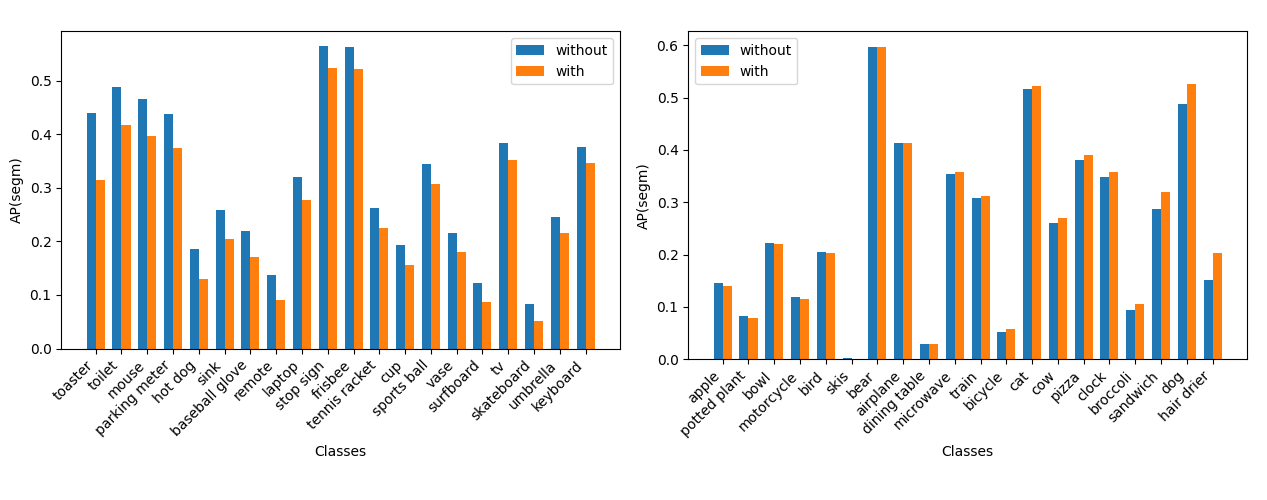
\includegraphics[width=1.05\textwidth]{Images/main/overlap_classes.png}
	\caption[\textbf{Training without overlapping instances - Class wise comparison}]{\textbf{Class wise comparison} of change in \(AP_{segm}\) of models trained using images with and without overlapping instances evaluated on COCO Eval dataset - 20 most and least improved classes}
	\label{fig:overlap_classes}
\end{figure*}

To ensure that the observed improvements in performance were not simply due to the loss of accuracy in one class being offset by gains in another, class-wise improvements are calculated on the COCO Eval dataset. This analysis allows for a more granular understanding of the model’s performance across different classes. By evaluating each class individually, we can verify that the enhancements in instance detection and segmentation are consistent and not merely the result of compensatory effects between classes. This class-wise assessment provides a clearer picture of the model's true capabilities, ensuring that the overall performance gains are robust and evenly distributed across the dataset.

The test results are illustrated in Fig.~\ref{fig:overlap_classes}, which highlights the 20 classes with the most significant improvements and the 20 classes with the least improvements in the COCO Eval dataset, based on the Average Precision for instance segmentation. Notably, our approach outperforms the baseline across the majority of classes. Specifically, it performs better in 68 out of the 80 classes assessed. In contrast, for the remaining 12 classes, our method shows reduced performance relative to the baseline. This distribution underscores the effectiveness of our approach in enhancing instance segmentation performance across a broad range of classes, with only a few exceptions where it falls short.

\subsection{Proposed Mask Filtering Method}
\label{section:mask_refinement_experiment}
To address the issue of unwanted background masks included in the pseudo-ground truths, we introduce an enhanced mask filtration approach. This section details the experimental setup and results associated with our improved mask filtration technique.

\subsubsection{Dataset}
We use the ImageNet dataset for training and evaluate on COCO, KITTI, PASCAL VOC 2012, Comic and Watercolor datasets. During the initial phase of training, both the baseline and our proposed method utilize the full set of images from ImageNet. However, after the first round of mask filtration in our method, approximately 10\% of the images are discarded due to the absence of usable masks. Consequently, the corresponding MaskCut annotations for these excluded images are also removed and the rest 90\% images constitute the training dataset for the second stage.

\subsubsection{Training Procedure}
The baseline follows training procedure as described in section~\ref{section:implementation_details}. But our method comes with once extra step of refining MaskCut masks using our modified mask filtration method explained in section~\ref{section:proposed_method} and training from scratch again. This is followed self-training as employed in the baseline to improve the performance further. We train both models using 4 and 8 batch sizes to analyze the influence of batch size on performance of the model (Section~\ref{section:choice_of_batch_size}). 

\subsubsection{Results}
\begin{table}[htbp]
	\centering
	\resizebox{1.05\textwidth}{!}{%
		\begin{tabular}{c|c|cc|cc|cc|cc|cc}
			\toprule
			& & \multicolumn{2}{c|}{COCO} & \multicolumn{2}{c|}{KITTI} & \multicolumn{2}{c|}{VOC} & \multicolumn{2}{c|}{Comic} & \multicolumn{2}{c}{Watercolor} \\ \midrule
			& & AP & AP50 & AP & AP50 & AP & AP50 & AP & AP50 & AP & AP50 \\ \midrule
			\multirow{2}{*}{Train} & Baseline & 11.17 & 20.12 & 4.79 & 10.27 & 19.98 & 36.26 & \textbf{11.80} & \textbf{28.39} & \textbf{14.67} & \textbf{35.60} \\ 
			& Ours & \textbf{11.47} & \textbf{20.81} & \textbf{6.28} & \textbf{13.48} & \textbf{20.24} & \textbf{36.56} & 10.81 & 26.50 & 14.00 & 35.27 \\ \midrule
			\multirow{2}{*}{r1} & Baseline & 11.70 & 21.15 & 6.60 & 14.19 & 19.56 & 36.81 & \textbf{11.05} & \textbf{27.53} & 12.92 & 33.45 \\ 
			& Ours & \textbf{11.94} & \textbf{21.65} & \textbf{8.21} & \textbf{18.49} & \textbf{20.24} & \textbf{37.95} & 10.80 & 27.40 & \textbf{15.37} & \textbf{37.74} \\ \midrule
			\multirow{2}{*}{r2} & Baseline & \textbf{11.02} & 20.32 & 6.73 & 15.02 & \textbf{18.06} & 35.09 & \textbf{9.90} & \textbf{25.36} & \textbf{13.59} & \textbf{34.31} \\ 
			& Ours & 10.81 & \textbf{20.47} & \textbf{7.69} & \textbf{17.04} & 17.93 & \textbf{35.24} & 8.94 & 22.74 & 12.06 & 30.02 \\ \bottomrule
		\end{tabular}%
	}
	\caption[\textbf{\(AP_{box}\) and \(AP50_{box}\) for Training and Self-Training}]{\textbf{\(AP_{box}\) and \(AP50_{box}\) for Training and Self-Training} evaluated on COCO Eval dataset (Batch size 8)}
	\label{tab:combined_train}
\end{table}

\begin{table}[htbp]
	\centering
	\resizebox{1.05\textwidth}{!}{%
		\begin{tabular}{c|c|cc|cc|cc|cc|cc}
			\toprule
			& & \multicolumn{2}{c|}{COCO} & \multicolumn{2}{c|}{KITTI} & \multicolumn{2}{c|}{VOC} & \multicolumn{2}{c|}{Comic} & \multicolumn{2}{c}{Watercolor} \\ \midrule
			& & AP & AP50 & AP & AP50 & AP & AP50 & AP & AP50 & AP & AP50 \\ \midrule
			\multirow{2}{*}{Train} & Baseline & 11.17 & 20.12 & 4.79 & 10.27 & 19.98 & 36.26 & \textbf{11.80} & \textbf{28.39} & \textbf{14.67} & \textbf{35.60} \\ 
			& Ours & \textbf{11.47} & \textbf{20.81} & \textbf{6.28} & \textbf{13.48} & \textbf{20.24} & \textbf{36.56} & 10.81 & 26.50 & 14.00 & 35.27 \\ \midrule
			\multirow{2}{*}{r1} & Baseline & 11.70 & 21.15 & 6.60 & 14.19 & 19.56 & 36.81 & \textbf{11.05} & \textbf{27.53} & 12.92 & 33.45 \\ 
			& Ours & \textbf{11.94} & \textbf{21.65} & \textbf{8.21} & \textbf{18.49} & \textbf{20.24} & \textbf{37.95} & 10.80 & 27.40 & \textbf{15.37} & \textbf{37.74} \\ \midrule
			\multirow{2}{*}{r2} & Baseline & \textbf{11.02} & 20.32 & 6.73 & 15.02 & \textbf{18.06} & 35.09 & \textbf{9.90} & \textbf{25.36} & \textbf{13.59} & \textbf{34.31} \\ 
			& Ours & 10.81 & \textbf{20.47} & \textbf{7.69} & \textbf{17.04} & 17.93 & \textbf{35.24} & 8.94 & 22.74 & 12.06 & 30.02 \\ \bottomrule
		\end{tabular}%
	}
	\caption[\textbf{\(AP_{segm}\) and \(AP50_{segm}\) for Training and Self-Training}]{\textbf{\(AP_{segm}\) and \(AP50_{segm}\) for Training and Self-Training} evaluated on COCO Eval dataset (Batch size 8)}
	\label{tab:combined_train_segm}
\end{table}

In this section, we present the results of our experiments comparing the baseline approach with our enhanced mask filtration method. Our evaluations span across five datasets, including COCO 2017 Evaluation, KITTI, VOC, Comic, and Watercolor, focusing on instance detection and segmentation tasks. We utilized the precision metric to measure the performance, providing a granular analysis of how our method impacts the accuracy of bounding box and segmentation predictions.

The results are summarized in Table~\ref{tab:combined_train} demonstrate the performance of both the baseline and our proposed method across different stages of training: the initial training phase and subsequent self-training iterations (r1 and r2). This table provides a comprehensive comparison of the model’s effectiveness on various datasets, shedding light on the strengths and weaknesses of each approach throughout the training process. 

During the initial training phase, our method outperforms the baseline on the majority of the datasets, including COCO, KITTI, and VOC. Specifically, we observe a notable improvement in precision metrics, indicating that our refined mask filtration process is effective in enhancing the quality of pseudo-ground truths, leading to better detection and segmentation performance. However, our model slightly underperforms on the Comic and Watercolor datasets. After the first round of self-training, our model continues to outperform the baseline on 4 out of 5 datasets. In the second round of self-training, we observe a slight decline in performance across most datasets for both the baseline and our method, except for minor improvements in the baseline on the KITTI and Watercolor datasets. This decline could be attributed to overfitting or the model’s diminishing returns from further self-training iterations, especially when using smaller batch sizes, as noted in our experiments in section~\ref{section:choice_of_batch_size}.

The evaluation on the Watercolor and Comic datasets has been somewhat inconsistent for both the baseline and our method. We hypothesize that this inconsistency arises from the stark difference between the types of images in these datasets compared to those in ImageNet. While our training predominantly involved real-life images, the Comic and Watercolor datasets consist of stylized, artistic images that pose a different challenge for the models. This disparity in image types likely contributes to the observed inconsistencies in performance.
%
%\begin{table}[htbp]
%	\centering
%	\begin{tabular}{c|c|c|cl}
%		\toprule
%		Eval dataset & Imagenet-all & Imagenet-wo-ol & Imagenet-maskcut-filter \\
%		\midrule
%		Coco Eval & 10.35, 19.15 & 11.52, 20.67 & 11.44, 21.31 \\
%		\midrule
%		Coco Eval w/o overlapping inst. & 23.45, 38.11  & 24.77, 39.46 & 24.64, 40.64 \\
%		\midrule
%		Coco Eval only overlapping inst. & 7.25, 15.11 & 8.52, 16.8 & 8.32, 17.28 \\
%		\bottomrule
%	\end{tabular}
%	\caption{\textbf{AP and AP50 of evaluation(box) on COCO Eval datasets on models trained on imagenet for 90K iterations}}
%	\label{tab:ablationK}
%\end{table}
%
%\begin{table}[htbp]
%	\centering
%	\begin{tabular}{c|c|c|cl}
%		\toprule
%		Eval dataset & Imagenet-all & Imagenet-wo-ol & Imagenet-maskcut-filter \\
%		\midrule
%		Coco Eval & 7.87, 16.05 & 8.80, 17.47 & 9.1, 18.15 \\
%		\midrule
%		Coco Eval w/o overlapping inst. & 19.19, 35.19  & 20.13, 36.36 & 21.15, 38.31 \\
%		\midrule
%		Coco Eval only overlapping inst. & 5.12, 11.55 & 6.18, 13.27 & 9.78, 18.92 \\
%		\bottomrule
%	\end{tabular}
%	\caption{\textbf{AP and AP50 of evaluation(segm) on COCO Eval datasets on models trained on imagenet for 90K iterations}}
%	\label{tab:ablationK}
%\end{table}

\subsection{Choice of batch size}
\label{section:choice_of_batch_size}

\begin{table}[htbp]
	\centering
	\begin{tabular}{c|c|cc|cc}
		\toprule
		& & \multicolumn{2}{c|}{Batch size = 8} & \multicolumn{2}{c}{Batch size = 4} \\ \midrule
		& & AP & AP50 & AP & AP50 \\ \midrule
		\multirow{2}{*}{Train} & Baseline & 11.17 & 20.12 & 10.74 & 19.78 \\ 
		& Ours & \textbf{11.47} & \textbf{20.81} & \textbf{11.66} & \textbf{21.33} \\ \midrule
		\multirow{2}{*}{Self-train-r1} & Baseline & 11.70 & 21.15 & 11.35 & 21.23 \\ 
		& Ours & \textbf{11.94} & \textbf{21.65} & \textbf{11.79} & \textbf{21.58} \\ \midrule
		\multirow{2}{*}{Self-train-r2} & Baseline & \textbf{11.02} & 20.32 & 10.51 & 20.03 \\ 
		& Ours & 10.81 & \textbf{20.47} & \textbf{11.25} & \textbf{20.20 }\\ \bottomrule
	\end{tabular}
	\caption[\textbf{\(AP_{box}\) and \(AP50_{box}\) for Training and Self-Training} for different batch sizes]{\textbf{\(AP_{box}\) and \(AP50_{box}\) for Training and Self-Training} evaluated on COCO Eval dataset  for batch sizes 4 and 8}
	\label{tab:batch_size_table}
´\end{table}

In the baseline paper, experiments were conducted using a batch size of 16. However, due to resource limitations, we performed our experiments with smaller batch sizes of 4 and 8. As shown in Table~\ref{tab:batch_size_table}, our results indicate a slight improvement in performance with a larger batch size, consistent with expectations that batch size can impact model performance.

Specifically, we observed that for both batch sizes of 4 and 8, the performance of our method and the baseline improved after the first round of self-training (r1) but declined in the second round (r2). This pattern diverges from the findings in the baseline paper, where using a batch size of 16 led to continued performance improvement through the second round of self-training. The observed performance drop in the second self-training round at smaller batch sizes suggests that batch size plays a crucial role in stabilizing the training process, potentially by providing more robust gradient estimates or better generalization.

Furthermore, the influence of batch size on the relative gains achieved through self-training is evident in our experiments. Larger batch sizes tend to offer a more stable training environment, which may explain the continued improvement seen in the baseline paper with a batch size of 16. Conversely, the smaller batch sizes used in our experiments may introduce greater variance, leading to less consistent performance gains across self-training rounds. This highlights the importance of considering batch size as a key factor in optimizing training pipelines for tasks involving self-training and iterative refinement.

%\subsection{\ad}
%ADE20K, introduced by  Zhou et al., provides detailed annotations for pixel-level segmentation, covering both objects and stuff categories \cite{zhou2017scene}. The dataset is split into a training set and a validation set. The training set consists of approximately 20,000 images, while the validation set contains around 2,000 images. ADE20K is known for its comprehensive coverage of scenes and contains annotations for 150 object classes and 92 stuff categories, making it a valuable resource for zero-shot semantic segmentation in our experiments.
%
%\section{Evaluation Metric}
%\subsection{\mIoU}
%The Mean Intersection over Union (mIoU) is a widely employed evaluation metric within the field of computer vision, specifically designed for the assessment of semantic segmentation models. It quantifies the degree to which the predicted segmentation masks align with the ground truth annotations for a given semantic segmentation task involving N classes. This alignment is determined by comparing the prediction logits and ground truth logits for a specific class, denoted as `c', based on three key parameters: (i) True Positive (TP(c)): Number of pixels correctly classified as class c, (ii)False Positive (FP(c)): Number of pixels incorrectly classified as class c but should belong to other classes, (iii)
%False Negative (FN(c)): Number of pixels incorrectly classified as other classes but should belong to class c. The IoU for a specific class `c' is calculated as shown in the below Eq. \ref{eq:IoU}
%\begin{equation}
%\label{eq:IoU}
%    \text{IoU}(c) = \frac{\text{TP}(c) + \text{FP}(c) + \text{FN}(c)}{\text{TP}(c)} ,
%\end{equation}
%The final mIoU is then obtained by calculating the mean across all classes as shown in the below Eq. \ref{eq:miou} to calculate the final mIoU.
%\begin{equation}
%    \label{eq:miou}
%    mIoU = \frac{1}{N} \sum_{c=1}^{N} IoU(c),
%\end{equation}
%This metric allows researchers to effectively evaluate the performance of their semantic segmentation models and assess how well the model aligns with the ground truth
%
%
%\section{Experiment Setting}
%\label{sec:experiment}
%
%The GroupViT model is trained on a combination of CC12M and filtered YFCC datasets, amounting to a total of 26 million image-text pairs \cite{changpinyo2021conceptual, thomee2016yfcc100m}. This training spans 30 epochs and employs 16 NVIDIA V100 GPUs over a 2-day period, utilizing a batch size of 4096. The initial two epochs serve as warm-up stages, gradually increasing the learning rate from an initial value of $4 \times 10^{-6}$ to reach a base of $1.6 \times 10^{-3}$. The training process integrates a weight decay of 0.05 to counter overfitting, and gradient clipping to prevent gradient magnitudes exceeding 5.0. Employing the AdamW optimizer with epsilon set at $1 \times 10^{-8}$ and beta coefficients of 0.9 and 0.999, a cosine learning rate scheduler is employed \cite{kingma2014adam, loshchilov2016sgdr}.\\
%For our experiments, we always train the pretrained model on MSCOCO. \textit{In this context, we use `training' and `fine-tuning' interchangeably}. With a global batch size of 256, we introduce a learning rate scale of 0.01 to adjust minimum and warm-up learning rates, aiding convergence. The warm-up epoch of 1 allows gradual increase of initial learning rate. A cosine scheduler over 12 decay epochs is used, gradually reducing the learning rate with 2 cycles of annealing for refinement. If not explicitly mentioned, we use 2 NVIDIA 1080Ti GPUs for our training procedure. We use seed `123' for reproducibility if it is not explicitly mentioned.\\
%For inference, we keep an image resolution of 448, stride of 224 and crop size of 448. For background threshold, we use 0.95 for PASCAL VOC, 0.9 for COCO, 0.35 for \pcon and 0.95 for ADE20K. Note that authors of GroupViT do not evaluate on ADE20K. Therefore, we keep all settings unchanged and use the background threshold as determined by the authors of OVSegmentator \cite{xu2023learning}. We  do an ablation on these inference settings for our baseline to report the best possible setting in section \ref{sec:infsettings}
%% 
%\begin{document}
\begin{table}[htbp]
\label{tab:hp}
  \centering
  \begin{tabular}{c|c}
    \toprule
    \textbf{Hyperparameter} & \textbf{Value} \\
    \midrule
    Training Epochs & 30 \\
    \midrule
    Warmup Epochs & 0\\
    \midrule
    Batch Size & 4096 \\
    \midrule
    Learning rate(LR) scheduler &  Cosine\\
    \midrule
    Minimum LR & $4e^{-5}$ \\
    \midrule
    Warmup LR & $4e^{-6}$ \\
    \midrule
    Base LR & 0.0016\\
    \midrule
    Optimizer &  AdamW\\
    \midrule
    Weight decay & 0.05 \\
    \midrule
    Number of nouns to extract(K) & 3 \\
    \midrule
    Number of stages & 3 \\
    \midrule
    Number of transformer block on each stage & 6, 3, 3 \\
    \midrule
    Group tokens on every stage & 64, 8, 0\\
    \midrule
    Number of heads in transformer block & 6, 6, 6\\
    \midrule
    Vision Encoder embedding dimension & 384\\
    \midrule
    Number of Transformer blocks in Text encoder & 12\\
    \midrule
    Text Encoder embedding dimension & 256\\
    \midrule
    Context Length  & 77\\
    \midrule
    Vocabulary size  & 49408\\
    \midrule
    Multimodal space embedding dimension & 256\\
    \midrule
    Contrastive loss temperature  & 0.07\\
    \bottomrule
    
  \end{tabular}
  
  \caption{GroupViT  Hyperparameters}
\end{table}


%\end{document}
%% %\begin{document}
\begin{table}[htbp]
\label{tab:infhp}
  \centering
  \begin{tabular}{c|c}
    \toprule
    \textbf{Inference Hyperparameter} & \textbf{Value} \\
    \midrule
    Image resolution & 448 \\
    \midrule
    mode & slide\\
    \midrule
    stride & 224 \\
    \midrule
    crop size   & 448\\
    \midrule
    Background threshold & \pvoc(0.95) \\
                    & \pcon(0.35) \\
                    & \coco(0.9) \\
                    & \ad(0.95)\\
    \bottomrule
    
  \end{tabular}
  
  \caption{GroupViT Inference Hyperparameters}
\end{table}


%\end{document}
%
%\section{ Visual Grouping vs Visual-Text Alignment}
%\label{sec:analyse}
%In our quest to enhance the performance of the GroupViT approach and identify its limitations, we conduct a comprehensive analysis using the PASCAL VOC dataset. Within GroupViT, the Semantic Segmentation task consists of two key subtasks: visual grouping and visual-language alignment. To precisely identify GroupViT's limitations, we perform two distinct sets of experiments. In each set, we isolate and evaluate these subtasks individually.
%\subsection{Analysis of Visual Grouping}
%In the first set of experiments, we evaluate GroupViT's performance exclusively on the Visual Grouping task. We refrain from using GroupViT's labeling mechanism and instead propose an alternative approach, as explained below.
%
%\subsubsection{Feature Extraction}
%We extract features using the pretrained GroupViT model for the training split of the Pascal VOC 2012 dataset. Images are processed through the visual encoder with frozen weights, where they are grouped into 8 segments in the final stage. We use features from the final stage, denoted as ${\hat{S}_i^{3}}$, to build a feature bank represented as $\mathbb{F} \in \mathbb{R}^{|\hat{S}^3| \times D}$. In our setup, $D$ represents the visual encoder's dimension, which is 384, and $|\hat{S}^3|$ represents the number of segment tokens obtained after the final stage, which is 8. This configuration results in 8 features per image. For our experiment, the feature bank contains a total of 11,592 features.
%
%\subsubsection{Soft Label Assignment}
%To label the features, we deviate from GroupViT's label assignment method. Similar to the inference process outlined in Section \ref{sec:inf}, we compute the global soft attention of group tokens, denoted as $\text{\textbf{Attn}} \in \mathbb{R}^{|G^2| \times |S^1|}$, as shown in Eq. \ref{eq:globalsoftattn}. The attention map is then reshaped into a $|G^2| \times P \times P$ format, where $P \times P$ corresponds to a $16 \times 16$ patch token format. We use bilinear interpolation to resize the map to $G^2 \times H \times W$, where $H$ and $W$ represent the image's height and width. By performing an argmax operation, we assign pixels to specific groups, resulting in a 2D vector of size $H \times W$ that indicates group associations, as demonstrated in Eq. \ref{eq:argmaxsecondlevelgrouping}. This process yields a segmented image.
%
%% \begin{equation}
%% \label{eq:secondlevelgrouping}
%%     \hat{X} = 
%% \end{equation}
%\begin{equation}
%\label{eq:argmaxsecondlevelgrouping}
%    \text{Segmented\_Image} = \text{Argmax}(\text{Interpolate}(\textbf{Attn}))
%\end{equation}
%To label the segments in the obtained segmented image, we extract their corresponding labels from the ground truth mask, denoted as M. To address cases where some pixels of a feature are labeled as class `A' while others are labeled as class `B,' we implement a soft label assignment approach. This method captures varying degrees of association, offering a more flexible representation of visual content.
%
%To achieve this, we maintain a soft label vector $S \in \mathbb{R}^{|\hat{S}^3| \times (N+1)}$, where $|\hat{S}^3|$ is the number of segments, and $N+1$ represents the class count, including the background class. For instance, in the case of Pascal VOC 2012 with 21 classes, each image feature is associated with a 21-sized array, where the indices correspond to class assignments. If all the pixels of a feature  belong to class `A', the corresponding index is set to 1. When out of N pixels, X pixels belong to class `A' and (N-X) pixels belong to class `B', the indices for class `A' and class `B' would have values X/N and (N-X)/N, respectively. Each index ideally represents the percentage of segment area associated with a specific class.
%
%\subsubsection{Find K-Nearest Neighbors (KNN)} 
%After obtaining soft labels for the features, our goal is to train a K-Nearest Neighbors (KNN) model \cite{cover1967nearest}. To ensure balanced features, we set a maximum limit of 1000 features for each category. We also conducted ablation experiments on the value of K, as shown in Table \ref{tab:ablationK}, and present the results in Table \ref{tab:analyssiresult}.
%
%\subsubsection{Evaluation}
%To evaluate the validation set, we follow the same procedure as for the training set to extract group token features. Let $V$ be the set of images in the validation set. For each image $v \in V$, we extract features of its segment tokens $F_v = {f_{v1}, f_{v2}, \ldots, f_{v8}}$, where $f_{vi}$ represents the $i$th segment token feature of image $v$.
%
%Next, we find the nearest neighbors for each feature in the validation set. We use $T$ to denote the bag of features obtained from the training set. For each segment token feature $f_{vi}$ of an image $v$, we find its $k$ nearest neighbors $KNN_{vi} = {t_{vi1}, t_{vi2}, \ldots, t_{vik}}$ from $T$. We aggregate their corresponding soft labels $S_{vik}$ using the mean operation:
%
%\begin{equation}
%\label{eq:analysisaggre}
%\overline{S_{vi}} = \frac{1}{k} \sum_{t_{vik} \in {KNN}{vi}} S_{vik}
%\end{equation}
%
%We then apply the argmax operation to the aggregated soft labels $\overline{S_{vi}}$ to obtain the final label $y_{vi}$ for each segment token feature $f_{vi}$:
%
%\begin{equation}
%\label{eq:labelassign}
%y_{vi} = \arg\max(\overline{S_{vi}})
%\end{equation}
%
%This process provides us with the final labels for all segment token features in the validation set. Using these labels, we obtain the segmentation logits and evaluate the segmentation results using the mean Intersection over Union (mIoU) metric. The results are presented in Table \ref{tab:analyssiresult}.
%
%In summary, the procedure entails the extraction of segment token features from the final stage for the training split of the PASCAL VOC dataset to create a bag of features. We fit a KNN model on these features. We then extract the features for the validation split. Nearest neighbors are identified for all the features, and soft labels are aggregated, allowing for the assignment of final labels. We then obtain segmentation logits, and evaluate the mIoU score on the dataset. This holistic process offers valuable insights into the model's performance in terms of visual grouping.
%
%
%\subsection{Analysis of Vision-Text Alignment}
% 
%We analyze the performance of the Vision-Text alignment mechanism of \gvit on \pvoc without utilizing visual grouping, relying solely on ground truth masks. Following the inference pipeline in Section \ref{sec:inf}, we compute the metric $\textbf{L}_{affinity} \in \mathbb{R}^{ H \times W \times N }$ as defined in Eq. \ref{eq:pred}, where H and W represent the image's height and width, respectively, and N is the number of classes.
%
%Next, we load the ground truth mask for an image, where each pixel is labeled with its associated class, including the background. Let $M$ be the ground truth mask, with each entry $M_{i,j}$ representing the class label at pixel $(i,j)$. For each class $c$ in $M$, we gather all pixels belonging to class $c$ in $\textbf{L}_{affinity}$ to identify groups in $\textbf{L}_{affinity}$ without employing \gvit's grouping mechanism. Specifically, all pixels associated with class `c' form a group, denoted as $G_c$. We calculate the mean of this group of pixels, $M_{G_c}$, along the last dimension (representing classes) to obtain a mean channel value for all pixels in the group. We then perform an argmax operation over the class channel to obtain $C_{G_c}$, as shown in Eq. \ref{eq:assignment}. Here, $C_{G_c}$ refers to the class assigned to all pixels in group $G_c$:
%
%\begin{equation}
%\label{eq:mean}
%M_{G_c} = \frac{1}{|G_c|} \sum_{p=1}^{|G_c|} \textbf{L}_{affinity}(p)
%\end{equation}
%
%\begin{equation}
%\label{eq:assignment}
%C_{G_c} = \text{Argmax}( M_{G_c})
%\end{equation}
%% \begin{equation}
%% \label{eq:variance}
%% V_{G_c} = \frac{1}{|G_c|} \sum_{p=1}^{|G_c|} (\textbf{L}_{\text{affinity}}(p) - M_{G_c})^2
%% \end{equation}
%
%We then label all associated pixels with the obtained class $C_{G_c}$. This way, we identify groups by grouping all pixels belonging to the same class based on the ground truth mask, without using the grouping mechanism of \gvit. We assign class labels using the GroupViT mechanism, and the results are presented in Table \ref{tab:analyssiresult}. 
%We note that while Visual Grouping and Visual-Text alignment both outperform GroupViT individually, it is evident that Visual Grouping exhibits a larger potential for improvement compared to alignment. We also conducted an evaluation without the background class to report the mIoU score, eliminating the reliance on the susceptibility of the background threshold.
%
%% Additionally, we calculate the variance, $V_{G_c}$, as shown in Eq. \ref{eq:variance}, to measure the variance of Intersection over Union (IoU) for different categories. We observe higher variance for categories like `person' `monitor' and `table' compared to others. This variance is likely due to visual differences caused by varying orientations and appearances. For example, `monitor' may have different displays in different images, contributing to higher visual variance. `Person' may share the scene with various complementary objects, leading to increased variance.
%\begin{figure*}
%
%  %   \begin{tabular}{ccccc}
%  %   \textbf{Image} & \textbf{Column 2} & \textbf{Column 3} & \textbf{Column 4} &    \textbf{Ground Truth}\\
%  % \end{tabular}
%  \centering
%   % \rotatebox{45}{\textbf{\footnotesize  Image}}\hfill
%   % \rotatebox{45}{\textbf{\footnotesize Visual-Text alignment}}\hfill
%   % \rotatebox{45}{\textbf{\footnotesize Visual Grouping}}\hfill
%   % \rotatebox{45}{\textbf{\footnotesize GroupViT}}\hfill
%   % \rotatebox{45}{\textbf{\footnotesize Ground-Truth}}
%  % \subfloat {\textbf{\footnotesize Image}}
%  % \hfill
%  % \subfloat {\textbf{\footnotesize  \ \ \ \ \ \ Visual-Text}}
%  % \hfill
%  % \subfloat {\textbf{\footnotesize Visual}}
%  % \hfill
%  % \subfloat {\textbf{\footnotesize GroupViT}}
%  % \hfill
%  % \subfloat {\textbf{\footnotesize Ground-Truth}}
%  
%  % \vspace{-0.1em}
%  
%  % \subfloat {\textbf{}}
%  % \hfill
%  % \subfloat {\textbf{\footnotesize \ Alignment}}
%  % %\hfill
%  % \subfloat {\textbf{\footnotesize \ \ \ \ \ \ \ \ \ Grouping}}
%  % \hfill
%  % \subfloat {\textbf{}}
%  % \hfill
%  % \subfloat {\textbf{\footnotesize }}
%
%  % \vspace{-0.1em}
%  \subfloat {\textbf{\small \ \ Image}}
%  \hspace{4em}
%  \subfloat {\textbf{\small Alignment}}
%  \hspace{1.5em}
%  \subfloat {\textbf{\small Grouping}}
%  \hspace{1.5em}
%  \subfloat {\textbf{\small \ \ \ \ GroupViT}}
%  \hspace{2em}
%  \subfloat {\textbf{\small Ground-Truth}}
%  
%  \vspace{-0.02em} 
%  \vspace{-0.05em} 
%  %  \subfloat {\textbf{\small \ \ Image}}
%  % \hspace{4em}
%  % \subfloat {\textbf{\small \ \ \ Alignment}}
%  % \hspace{1.5em}
%  % \subfloat {\textbf{\small Grouping}}
%  % \hspace{1.5em}
%  % \subfloat {\textbf{\small GroupViT}}
%  % \hspace{1.5em}
%  % \subfloat {\textbf{\small \ \ \ \ Ground-Truth}}
%  % \vspace{-0.02em} 
%  % \vspace{-0.05em}
%  
%  {\includegraphics[width=0.19\textwidth]{Images/analysis/0000.jpg}}
%  {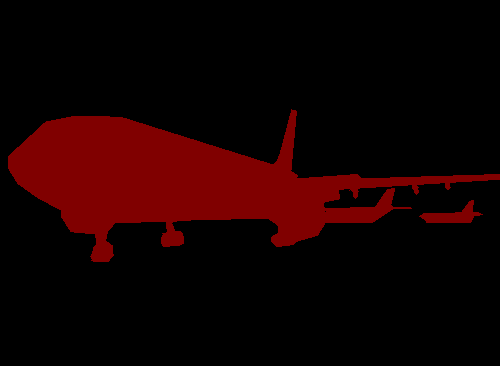
\includegraphics[width=0.19\textwidth]{Images/analysis/0.png}}
%  {
\includegraphics[width=0.19\textwidth]{Images/analysis/colored_mask_gi_val0.png}}
%  {
\includegraphics[width=0.19\textwidth]{Images/analysis/originalcheckpoint/0000.png}}
%  {
\includegraphics[width=0.19\textwidth]{Images/analysis/2007_000033.png}}
%  {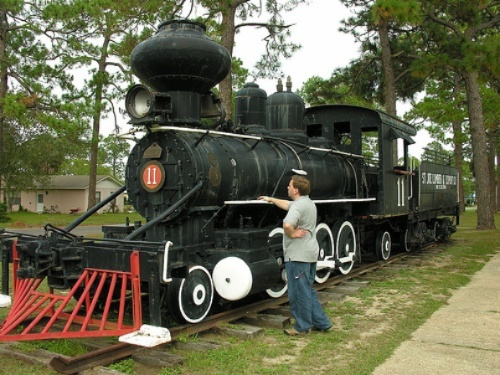
\includegraphics[width=0.19\textwidth]{Images/analysis/0081.jpg}}
%  {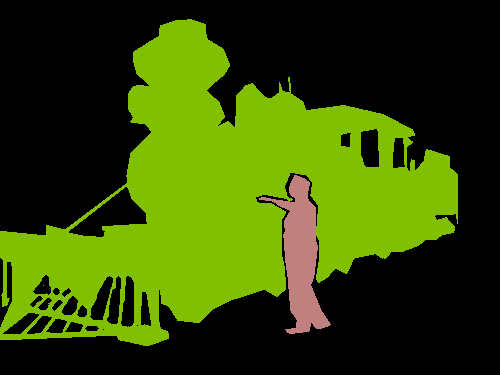
\includegraphics[width=0.19\textwidth]{Images/analysis/81.png}}
%  {
\includegraphics[width=0.19\textwidth]{Images/analysis/colored_mask_gi_val81.png}}
%  {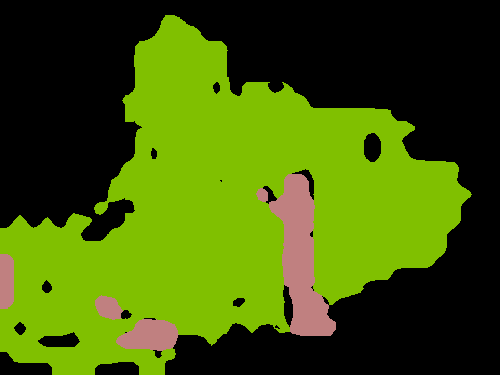
\includegraphics[width=0.19\textwidth]{Images/analysis/originalcheckpoint/0081.png}}
%  {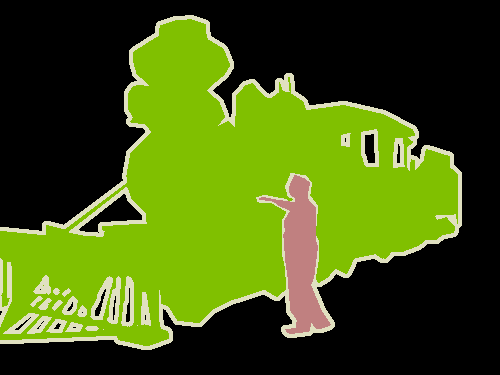
\includegraphics[width=0.19\textwidth]{Images/analysis/2007_002565.png}}
%  {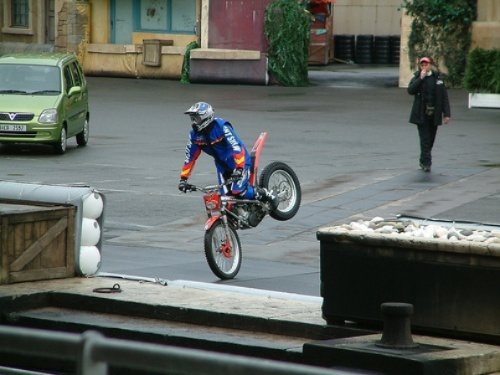
\includegraphics[width=0.19\textwidth]{Images/analysis/0086.jpg}}
%  {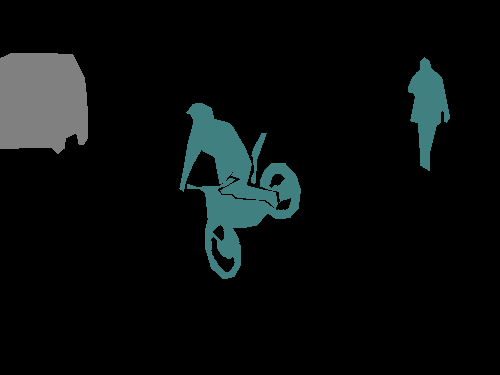
\includegraphics[width=0.19\textwidth]{Images/analysis/86.png}}
%  {
\includegraphics[width=0.19\textwidth]{Images/analysis/colored_mask_gi_val86.png}}
%  {
\includegraphics[width=0.19\textwidth]{Images/analysis/originalcheckpoint/0086.png}}
%  {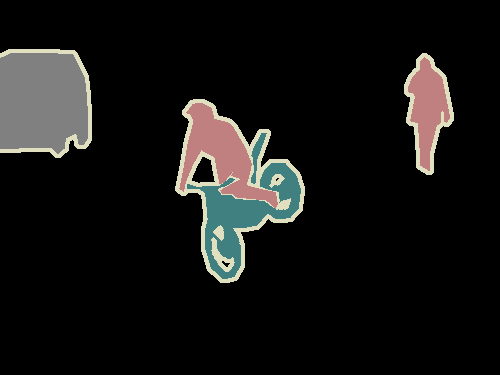
\includegraphics[width=0.19\textwidth]{Images/analysis/2007_002643.png}}
%  {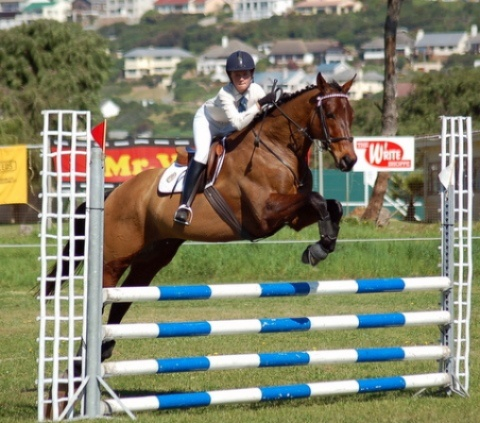
\includegraphics[width=0.19\textwidth]{Images/analysis/0262.jpg}}
%  {
\includegraphics[width=0.19\textwidth]{Images/analysis/262.png}}
%  {
\includegraphics[width=0.19\textwidth]{Images/analysis/colored_mask_gi_val262.png}}
%  {
\includegraphics[width=0.19\textwidth]{Images/analysis/originalcheckpoint/0262.png}}
%  {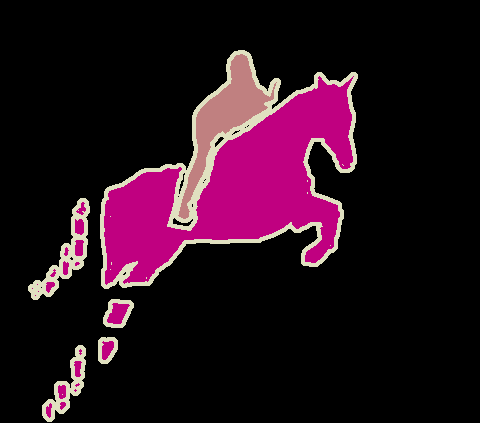
\includegraphics[width=0.19\textwidth]{Images/analysis/2007_008256.png}}
%  {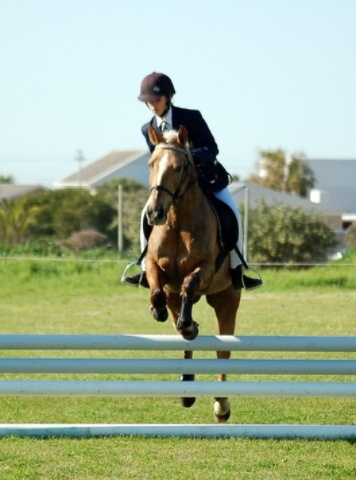
\includegraphics[width=0.19\textwidth]{Images/analysis/0270.jpg}}
%  {
\includegraphics[width=0.19\textwidth]{Images/analysis/270.png}}
%  {
\includegraphics[width=0.19\textwidth]{Images/analysis/colored_mask_gi_val270.png}}
%{
\includegraphics[width=0.19\textwidth]{Images/analysis/originalcheckpoint/0270.png}}
%  {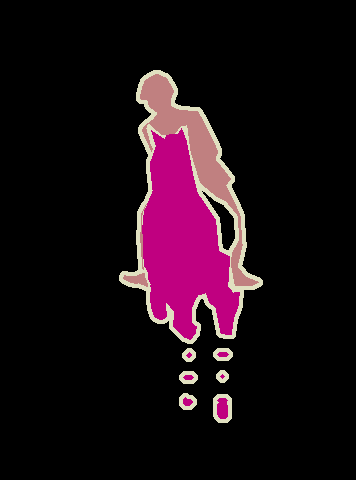
\includegraphics[width=0.19\textwidth]{Images/analysis/2007_008596.png}}
%\caption[\textbf{Visualization of Visual Grouping Vs Visual-Text Alignment}]{\textbf{Visualization of Visual Grouping Vs Visual-Text Alignment}. Comparison of Segmentation Masks using Different Models. The first and last columns show image and the corresponding ground truth segmentation masks, while the remaining columns display the segmentation masks generated by Visual-Text alignment, Visual grouping and the Original checkpoint.}
%    
%\end{figure*}
%
%
% \begin{table}[htbp]
% \begin{center}
%     \begin{tabular}{|c|c|c|}
%         \hline
%         Model &  Data & mIoU     \\ \hline
%         \gvit & \pvoc & $52.29$  \\
%         \gvit & \coco & $24.3$   \\
%         \ovs  & \pvoc & $53.78$  \\
%         \ovs  & \coco & $25.06$  \\
%         \hline
%     \end{tabular}
%     \end{center}

%     \caption[Table caption]{\textbf{Table caption.} foo bar...\\}
%     \label{tab:accuracy}
% \end{table}



\begin{table}[htbp]
  \centering
  
  \begin{tabular}{c|c|cl}
    \toprule
    Model & Type & \pvoc \\
    \midrule
    \gvit & Original & 52.29  \\
    \midrule
    \gvit & Visual Grouping  & 54.16  \\
    \midrule
    \gvit & Visual Grouping(WB)  & 56.12  \\
    \midrule
    \gvit & Visual-Text Alignment & \textbf{76.18}  \\
    \bottomrule
  \end{tabular}
  \caption[\textbf{Analysis of Visual Grouping and Visual-Text Alignment}]{\textbf{Analysis of Individual Components.} Here, `Visual Grouping (WB)' refers to the evaluation performed without considering the `background' class.}
  
 \label{tab:analyssiresult}
\end{table}


\begin{table}[htbp]
  \centering
  \begin{tabular}{c|c|cl}
    \toprule
    Model & K & \pvoc \\
    \midrule
    Visual Grouping & 5 & 51.85 \\
    \midrule
    Visual Grouping & 10  & 54.26  \\
    \midrule
    Visual Grouping & 15 & 51.93  \\
    \midrule
    Visual Grouping & 25 & 49.66  \\
    \bottomrule
  \end{tabular}
  \caption{\textbf{Ablation on number of nearest neighbors for Visual Grouping}}
 \label{tab:ablationK}
\end{table}


% \documentclass{article}
% \usepackage{booktabs}

% \begin{document}

% \begin{table}[htbp]
%   \centering
%   \caption{My Pretty Table}
%   \begin{tabular}{ccc}
%     \toprule
%     Column 1 & Column 2 & Column 3 \\
%     \midrule
%     Row 1, Cell 1 & Row 1, Cell 2 & Row 1, Cell 3 \\
%     Row 2, Cell 1 & Row 2, Cell 2 & Row 2, Cell 3 \\
%     Row 3, Cell 1 & Row 3, Cell 2 & Row 3, Cell 3 \\
%     \bottomrule
%   \end{tabular}
% \end{table}

% \end{document}
%
%% \todo{add observation, variation across each class, ablation over k, with and without background}
%
%
%\section{Fine-tuning the Pretrained Model}
%In the previous section, our feature analysis highlighted opportunities to enhance GroupViT's visual grouping capabilities. These insights have motivated us to explore its full potential further. However, GroupViT is a substantial model with 55 million parameters, trained on a large dataset. Starting training from scratch would be resource-intensive. Instead, we've chosen to fine-tune the pretrained model, leveraging the valuable knowledge it acquired during its initial training phase and its understanding of visual and linguistic concepts. This approach also helps accelerate convergence. Our fine-tuning process involves training on a smaller and cleaner dataset, MSCOCO. This dataset provides human-annotated captions, which are believed to offer richer information about the corresponding images compared to the web-scaled datasets used in pretraining.
%
%\subsection{Choice of Components}
%To comprehensively analyze the core components of GroupViT for segmentation, we propose fine-tuning the Grouping Blocks and MLP Projectors. This aims to improve visual grouping quality and alignment in an image-text pair. We systematically evaluate different combinations within the visual encoder and report results in Table \ref{tab:ft}. 
%The experiment was conducted over 15 epochs.
%We observe that tuning both Grouping Blocks results in better performance compared to the other combinations. This validates our earlier findings in Section \ref{sec:analyse}, where we identified a greater room for improvement in visual grouping.
%
%\begin{document}
\begin{table}[htbp]
  \centering
  \begin{tabular}{c|c|c|l|l|l}
    \toprule
    \multirow{2}{*}{Model} & Fine-tuned & \multicolumn{4}{c}{Datasets} \\
    %\cmidrule(lr){1-2} \cmidrule(lr){3-4}
    \cline{3-6}
    & components & COCO & PVOC & PContext & ADE20K \\
    \midrule
    \gvit & Original & 24.3  & \textbf{52.29} & 22.39 &  \textbf{8.59}\\
    \midrule
    \gvit & Both GBs & \textbf{26.15}  & 49.18 & 21.87 & 7.50 \\
    \midrule
    \gvit & 2nd GB & 25.79 & 49.15 & 21.71 & 7.69 \\
    \midrule
    \gvit & Both GBs  & 25.62 & 49.22 & \textbf{22.41} & 8.49\\
          & + Img Proj &  &  &  & \\
    \midrule
    \gvit & 2nd GB  & 25.79 & 50.90 & 22.33 & 8.25\\
     &  + Img Proj &  &  &  & \\ 
    \midrule
    \gvit & Both GBs +  & 25.05 & 48.33 & 22.39 & 7.61\\
    
     &  Projs &  &  &  & \\
    \midrule
    \gvit & 2nd GB + Projs &  25.04 & 47.94 & 21.7 & 7.67\\
    \midrule
    \gvit & Img Proj & 24.48 & 50.32 & 22.36 & 8.27\\
    % \midrule
    % \gvit & VE &  & & & \\
    \midrule
    \gvit & Projs & 24.49 & 50.24 & 21.87 & 8.15\\
    \bottomrule
    
  \end{tabular}
  
  \caption[\textbf{Choice of Architectural Components to Fine-tune}]{\textbf{Choice of Architectural Components to Fine-tune}. Here, `GBs' stands for Grouping Blocks, while `Img Proj' represents the Image Projector within the Visual Encoder. `Projs' refers to both the Text MLP Projector and the Image MLP Projector. `+' is used to represent a combination of components.}
  
\label{tab:ft}
\end{table}


%\end{document}

% \begin{table}[t]
%     \scriptsize
%     \centering
%     \caption{Assessment of Approaches}
%     \label{tab:multi_shape}
%     \setlength\tabcolsep{5.0pt}
%     \begin{threeparttable}
%         \begin{tabular}{c|c|c|c|c|c|c|c|c}
%             \toprule
%                 \multirow{2}{2.0cm}{GroupViT} &  \multirow{2}{.5cm}{\centering GB1} & \multirow{2}{.5cm}{\centering GB2} &\multirow{2}{.5cm}{\centering IP} 
%                 &\multirow{2}{.5cm}{\centering TP} & \multicolumn{4}{c}{Datasets} \\
%                 %\cmidrule(lr){1-2} \cmidrule(lr){3-4}        
%                 \cline{6-9}
%                 & &  &  & & COCO & PVOC & PContext & ADE20K \\

%                 \midrule
%                 %single shape + sum & 65 & 70 & 68 \\
%                  Original & - & - & - & - & 24.3  & \textbf{52.29} & 22.39 &  \textbf{8.59} \\
%                 \midrule
%                  %Img Proj
%                 \multirow{10}{*}{Fine-tuned} & - & - & - & \checkmark & 24.48 & 50.32 & 22.36 & 8.27 \\
%                 \cmidrule{2-9}
%                 %Text Proj
%                  & - & - & \checkmark & \checkmark & 24.49 & 50.24 & 21.87 & 8.15 \\
%                 \cmidrule{2-9}
%                 %2ndGB
%                  & - & \checkmark & - & - & 25.79 & 49.15 & 21.71 & 7.69  \\
%                 \cmidrule{2-9}
%                 %2ndGB + Img Proj
%                  & - & \checkmark & \checkmark & - & 25.79 & 50.90 & 22.33 & 8.25 \\
%                 \cmidrule{2-9}
%                 %2ndGB + Img Proj + Text Proj
%                 & - & \checkmark & \checkmark & \checkmark & 25.04 & 47.94 & 21.7 & 7.67 \\
%                 \cmidrule{2-9}
%                 %BothGBs
%                  & \checkmark & \checkmark & - & - &  \textbf{26.15}  & 49.18 & 21.87 & 7.50 \\
%                 \cmidrule{2-9}
%                 %BothGBs +ImgProj
%                  & \checkmark & \checkmark & \checkmark & - & 25.62 & 49.22 & \textbf{22.41} & 8.49 \\
%                 \cmidrule{2-9}
%                  %BothGBs +ImgProj + TextProj
%                  & \checkmark & \checkmark & \checkmark & \checkmark & 25.05 & 48.33 & 22.39 & 7.61 \\
                
%                 \bottomrule
%         \end{tabular}
%     \footnotesize
%     \vspace{.3em}
%     \hspace{-.11\linewidth}

%     \end{threeparttable}
%     \vspace{-0.3cm}
% \end{table}


% \begin{table}[t]
%     \scriptsize
%     \centering
%     \caption{}
%     \label{tab:multi_shape}
%     \setlength\tabcolsep{5.0pt}
%     \begin{threeparttable}
%         \begin{tabular}{c|c|c|c|c|c|c|c|c}
%             \toprule
%                 GroupViT &   GB1 & GB2 & IP & TP & COCO \\
%                 %\cmidrule(lr){1-2} \cmidrule(lr){3-4}        


%                 \midrule
%                 %single shape + sum & 65 & 70 & 68 \\
%                  Original & - & - & - & - & 24.3  & \textbf{52.29} & 22.39 &  \textbf{8.59} \\
%                 \midrule
%                  %Img Proj
%                 \multirow{10}{*}{Fine-tuned} & - & - & - & \checkmark & 24.48 & 50.32 & 22.36 & 8.27 \\
%                 \cmidrule{2-9}
%                 %Text Proj
%                  & - & - & \checkmark & \checkmark & 24.49 & 50.24 & 21.87 & 8.15 \\
%                 \cmidrule{2-9}
%                 %2ndGB
%                  & - & \checkmark & - & - & 25.79 & 49.15 & 21.71 & 7.69  \\
%                 \cmidrule{2-9}
%                 %2ndGB + Img Proj
%                  & - & \checkmark & \checkmark & - & 25.79 & 50.90 & 22.33 & 8.25 \\
%                 \cmidrule{2-9}
%                 %2ndGB + Img Proj + Text Proj
%                 & - & \checkmark & \checkmark & \checkmark & 25.04 & 47.94 & 21.7 & 7.67 \\
%                 \cmidrule{2-9}
%                 %BothGBs
%                  & \checkmark & \checkmark & - & - &  \textbf{26.15}  & 49.18 & 21.87 & 7.50 \\
%                 \cmidrule{2-9}
%                 %BothGBs +ImgProj
%                  & \checkmark & \checkmark & \checkmark & - & 25.62 & 49.22 & \textbf{22.41} & 8.49 \\
%                 \cmidrule{2-9}
%                  %BothGBs +ImgProj + TextProj
%                  & \checkmark & \checkmark & \checkmark & \checkmark & 25.05 & 48.33 & 22.39 & 7.61 \\
                
%                 \bottomrule
%         \end{tabular}
%     \footnotesize
%     \vspace{.3em}
%     \hspace{-.11\linewidth}

%     \end{threeparttable}
%     \vspace{-0.3cm}
% \end{table}
%\subsection{Choice of Batch Size}
%In our experiments, we change the global batch size to three different values: 256, 512, and 1024 and train the model for 10 epochs. In Table \ref{tab:batchsize}, we observe improved performance with a batch size of 1024 on \pvoc and PASCAL Context, while a batch size of 512 works best on COCO, as detailed in Table \ref{tab:batchsize}. While the literature suggests that a larger pool of negative samples can enhance contrastive loss outcomes \cite{jia2021scaling}\cite{radford2021learning}, it's also noted that large data scales are needed to counteract the impact of noisy image-text training \cite{jia2021scaling}. Our hypothesis aligns with our specific context: training on a relatively smaller yet cleaner dataset. This suggests that the noise introduced during training is not sufficiently mitigated, making a relatively smaller batch size of 512 a more effective choice. 
%% \begin{table}[htbp]
%   \centering

%   \begin{tabular}{ccc}
%     \toprule
%     Model & Batch Size & MSCOCO \\
%     \midrule
%     \gvit & 256 & \textbf{26.49} \\
%     \gvit & 512 & 26.4 \\
%     \gvit & 1024 & 26.16 \\
%     \bottomrule
%   \end{tabular}
%   \caption[\textbf{Choice of Batch Size}]{\textbf{Choice of Batch Size }}
%  \label{tab:batchsize}
% \end{table}

\begin{table}[htbp]
  \centering
  \begin{tabular}{c|c|c|l|l|l}
    \toprule
     \multirow{2}{*}{Model} & \multirow{2}{*}{Batch Size} & \multicolumn{4}{c}{Datasets} \\
    %\cmidrule(lr){1-2} \cmidrule(lr){3-4}
    \cline{3-6}
    &  & COCO & PVOC & PContext & ADE20K \\
    \midrule
    \gvit & 256 & 25.96 & 48.67 & 21.64 & 7.60\\
    %\gvit & VE& 45.46 & 21.44 \\
    \midrule
    
    \gvit & 512 & \textbf{26.13}   & 49.29 & 21.63 & \textbf{7.92}\\
    \midrule
    
    \gvit & 1024 & 25.92  & \textbf{49.73} & \textbf{21.71} & 7.57\\
    %\ovs  & GB + MMD & 53.78 & 25.06 \\
    \bottomrule
  \end{tabular}
  \caption[\textbf{Choice of Batch Size}]{\textbf{Choice of Batch Size }}
  \label{tab:batchsize}
\end{table}


%Due to resource constraints and only marginal differences in model performance across different batch sizes, we choose to proceed with a batch size of 256 for our experiments. However, as we observe some improvement with a batch size of 512, we will report the performance of our baseline, obtained later in Section \ref{sec:nncl}, using a global batch size of 512.
%
%
%\section{Exploring Impact of Multi-label}
%\label{sec:explabel}
%We investigate how extracted nouns affect performance, particularly their impact on embedding context. To enhance context, we extract comprehensive noun phrases from captions using NLTK and a regex expression. These phrases include adjectives before nouns and are denoted as `NP' in Table \ref{tab:texthierarchy}. Furthermore, we experiment with varying the number of extracted nouns and phrases (3, 5, 7 labels) to assess their effect on performance.
%
%In addition, we train a model without multi-label contrastive loss, and the results are shown in Table \ref{tab:texthierarchy}. Notably, we observe that the model trained on Noun Phrases, Nouns, and captions, with an upper limit of 5 on extracted labels, outperforms other settings. However, intriguingly, we observe similar performance for the model trained solely with contrastive loss and the one trained with both multi-label contrastive loss and contrastive loss.
%
%To provide a more robust analysis, we conduct experiments on 3 different seeds (0, 100, 200) for `NP+Nouns+Captions with 5 labels' and `Caption'. The results are summarized as mean and variance mIoU in Table \ref{tab:texthierarchy}. Visualizations in Figure \ref{fig:plot_text} confirmed convergence to similar performance, with slight initial speed-ups for multi-label training.
%
%As a result, we decide to proceed with the `NP+Nouns+Caption' model with 5 labels for subsequent experiments. This choice aligns with Xu et al.'s findings during GroupViT training \cite{xu2022groupvit}.
%
%
%

% \begin{table}[htbp]
% \begin{center}
%     \begin{tabular}{|c|c|c|}
%         \hline
%         Model &  Data & mIoU     \\ \hline
%         \gvit & \pvoc & $52.29$  \\
%         \gvit & \coco & $24.3$   \\
%         \ovs  & \pvoc & $53.78$  \\
%         \ovs  & \coco & $25.06$  \\
%         \hline
%     \end{tabular}
%     \end{center}

%     \caption[Table caption]{\textbf{Table caption.} foo bar...\\}
%     \label{tab:accuracy}
% \end{table}

% \begin{table}[htbp]
%   \centering
%   \caption{GroupViT - Ablation on Text hierarchy}
%   \begin{tabular}{cccc|l}
%     \toprule
%     Model & #labels & Text-Type & \multicolumn{2}{c}{Datasets} \\
%     \cmidrule(lr){1-3} \cmidrule(lr){4-5}
%     & &&\pvoc & \coco \\
%     \midrule
%     \gvit & 3 & Nouns+Caption & 49.65 & 26.32 \\
%     \gvit & 3 & NounPhrases+Noun+Caption & 50.24 & 26.35 \\
%     \gvit & 5 & NounPhrases+Noun+Caption & 50.16 & 26.5 \\
%     \gvit & 0 & Caption &  & 26.35 \\
%     \bottomrule
%   \end{tabular}
% \end{table}

% \begin{table}[htbp]
%   \centering
%   \begin{tabular}{ccc|c|l}
%     \toprule
%     Model & \#labels & Text-Type & \multicolumn{2}{c}{Datasets} \\
%     \cmidrule(lr){1-4} \cmidrule(lr){4-5}
%     & & & COCO & VOC\\
%     \midrule
%     \gvit & 3 & Nouns+Caption  & 26.32 & 49.65\\
%     \gvit & 3 & NP+Nouns+Caption & 26.35 & 50.24 \\
%     \gvit & 5 & NP+Nouns+Caption & \textbf{$26.74 \pm 0.0462$} & \textbf{$49.80 \pm 0.0042$}\\
%     \gvit & 7 & NP+Nouns+Caption  & 25.67 & 48.11 \\
%     \gvit & 0 & Caption  & $26.61 \pm 0.0175$ & \textbf{$51.79 \pm 0.0769$} \\
%     \bottomrule
%   \end{tabular}
%     \caption[\textbf{Exploring impact of Text hierarchy}]{\textbf{Exploring impact of Text hierarchy.}The model "NP+Nouns+Caption" extracts noun phrases and nouns for use in multi-label contrastive loss and captions for contrastive loss. While the model "Nouns+Caption" extracts just noun for use in multi-label contrastive loss. The model "Caption" is trained without multi-label contrastive loss  }
    
%   \label{tab:texthierarchy}
% \end{table}
% \begin{table}[htbp]
%   \centering
%   \begin{tabular}{c|c|c|c|llll}
%     \toprule
%     \multirow{2}{*}{Model} & \multirow{2}{*}{\#labels} &\multirow{2}{*}{Text-Type}& \multicolumn{2}{c}{Datasets} \\
%     \cline{4-7}
%       % \cmidrule(lr){4-5}
%     & & & COCO & VOC & Context & ADE20K\\
%     \midrule
%     \gvit & 3 & Nouns+Caption  & 26.32 & 49.65 & 22.04 & 7.95\\
%     \gvit & 3 & NP+Nouns+Caption & 26.35 & 50.24 & 22.09 & 8.17\\
%     \gvit & 5 & NP+Nouns+Caption & \textbf{26.74 $\pm$ 0.0462} & 49.80 $\pm$ 0.0042 & 21.92 $\pm$ 0.0061 & \\
%     \gvit & 7 & NP+Nouns+Caption  & 25.67 & 48.11 & 21.78 & 7.66 \\
%     \gvit & 0 & Caption  & 26.61 $\pm$ 0.0175 & \textbf{51.79 $\pm$ 0.0769} & 21.83 $\pm$ 0.0049 & \\
%     \bottomrule
%   \end{tabular}
%   \caption[\textbf{Exploring the Impact of Text Hierarchy}]{\textbf{Exploring the Impact of Text Hierarchy.} The model `NP+Nouns+Caption' extracts noun phrases and nouns for use in multi-label contrastive loss and captions for contrastive loss, while the model `Nouns+Caption' extracts only nouns for use in multi-label contrastive loss. The model `Caption' is trained without multi-label contrastive loss.}
%   \label{tab:texthierarchy}
% \end{table}
% \begin{table}[htbp]
%   \centering
%   \begin{tabular}{c|c|c|c|llll}
%     \toprule
%     \multirow{2}{*}{Model} & \multirow{2}{*}{\#labels} &\multirow{2}{*}{Text-Type}& \multicolumn{2}{c}{Datasets} \\
%     \cline{4-7}
%       % \cmidrule(lr){4-5}
%     & & & COCO & VOC & Context & ADE20K\\
%     \midrule
%     \gvit & 3 & Nouns+Caption  & 26.32 & 49.65 & 22.04 & 7.95\\
%     \gvit & 3 & NP+Nouns+Caption & 26.35 & 50.24 & 22.09 & 8.17\\
%     \gvit & 5 & NP+Nouns+Caption & \textbf{26.74 $\pm$ 0.0462} & 49.80 $\pm$ 0.0042 & 21.92 $\pm$ 0.0061 & \\
%     \gvit & 7 & NP+Nouns+Caption  & 25.67 & 48.11 & 21.78 & 7.66 \\
%     \gvit & 0 & Caption  & 26.61 $\pm$ 0.0175 & \textbf{51.79 $\pm$ 0.0769} & 21.83 $\pm$ 0.0049 & \\
%     \bottomrule
%   \end{tabular}
%   \caption[\textbf{Exploring the Impact of Text Hierarchy}]{\textbf{Exploring the Impact of Text Hierarchy.} The model `NP+Nouns+Caption' extracts noun phrases and nouns for use in multi-label contrastive loss and captions for contrastive loss, while the model `Nouns+Caption' extracts only nouns for use in multi-label contrastive loss. The model `Caption' is trained without multi-label contrastive loss.}
%   \label{tab:texthierarchy}
% \end{table}


\begin{table}[htbp]
  \centering
  \small % Reduce font size
  \setlength{\tabcolsep}{3.5pt} % Reduce column padding
  \begin{tabular}{c|c|c|c|c|c|c}
    \toprule
    \multirow{2}{*}{Model} & \multirow{2}{*}{\#labels} & \multirow{2}{*}{Type} & \multicolumn{4}{c}{Datasets} \\
    \cline{4-7}
    & & & COCO & PVOC & PContext & ADE20K\\
    \midrule
     \gvit(Original) & 3 & Nouns+caption &  24.3 & \textbf{52.29}  & \textbf{22.39} & \textbf{8.56}\\
     \midrule
    \multirow{2}{*}{\gvit} & \multirow{2}{*}{3} & Nouns & \multirow{2}{*}{26.32} & \multirow{2}{*}{49.65} & \multirow{2}{*}{22.04} & \multirow{2}{*}{7.95}\\
    & & +Caption& & & & \\
    \midrule
    \multirow{2}{*}{\gvit} & \multirow{2}{*}{3} & NP+Nouns & \multirow{2}{*}{26.35} & \multirow{2}{*}{50.24} & \multirow{2}{*}{\textbf{22.09}} & \multirow{2}{*}{\textbf{8.17}}\\
    & &+Caption & & & & \\
    \midrule
    \multirow{2}{*}{\gvit} & \multirow{2}{*}{5} & NP+Nouns & \textbf{26.74} & 49.80  & 21.92 & 7.42\\
    
    & & + Caption & \textbf{$\pm$ 0.0462} & $\pm$ 0.0042 & $\pm$ 0.0061 & $\pm$ 0.0022\\
   \midrule
    \multirow{2}{*}{\gvit} & \multirow{2}{*}{7} & NP+Nouns & \multirow{2}{*}{25.67} & \multirow{2}{*}{48.11} & \multirow{2}{*}{21.78} & \multirow{2}{*}{7.66} \\
    & & +Caption & & & & \\
   \midrule
    \multirow{2}{*}{\gvit} & \multirow{2}{*}{0} & \multirow{2}{*}{Caption} & 26.61 & 51.79 & 21.83  & 7.45 \\
    
    & & & $\pm$ 0.0175 & $\pm$ 0.0769 & $\pm$ 0.0049 & $\pm$ 0.0104\\
    
    \bottomrule
  \end{tabular}
  \caption[\textbf{Exploring the Impact of Text Hierarchy}]{\textbf{Exploring the Impact of Text Hierarchy.} The model `NP+Nouns+Caption' extracts noun phrases and nouns for use in multi-label contrastive loss and captions for contrastive loss, while the model `Nouns+Caption' extracts only nouns for use in multi-label contrastive loss. The model `Caption' is trained without multi-label contrastive loss.}
  \label{tab:texthierarchy}
\end{table}



% \begin{table}[t]
%     \scriptsize
%     \centering
%     \caption{Assessment of Approaches}
%     \label{tab:multi_shape}
%     \setlength\tabcolsep{5.0pt}
%     \begin{threeparttable}
%         \begin{tabular}{c|c|c|c|c|c|c|c|c}
%             \toprule
%                 % \multirow{2}{2.0cm}{GroupViT} &  \multirow{2}{1.5cm}{\centering Nouns} &\multirow{2}{1.5cm}{\centering Noun Phrases}&\multirow{2}{1.5cm}{\centering Caption} & \multirow{2}{1.5cm}{\centering \#Extracted Texts} &\multicolumn{4}{c}{Datasets} \\
%                 % %\cmidrule(lr){1-2} \cmidrule(lr){3-4}        
%                 % \cline{6-9}
%                 % & &  &  & & COCO & PVOC & PContext & ADE20K \\
%                 %\toprule
%                 GroupViT &  Noun & Noun Phrases & Caption & \#Extracted Texts & COCO \\
%                 %\cmidrule(lr){1-2} \cmidrule(lr){3-4}        


%                 \midrule
%                 %single shape + sum & 65 & 70 & 68 \\
%                  Original & \checkmark & - & \checkmark & 3 & 24.3  & \textbf{52.29} & \textbf{22.39} &  \textbf{8.59} \\
%                 \midrule
%                 \multirow{8}{*}{\centering Fine-tuned} & \checkmark & - & \checkmark& 3  & 26.32 & 49.65 & 22.04 & 7.95 \\
%                 \cmidrule{2-9}
%                 %GE
%                  & \multirow{4}{*}{\checkmark} & \multirow{4}{*}{\checkmark}  & \multirow{4}{*}{\checkmark}  & 3 & 26.35 & 50.24 & 22.09 & 8.17 \\
%                  %LE
%                  \cmidrule{5-9}
%                  &  &   & & 5 & \textbf{26.74} & 49.80  & 21.92 & 7.42\\
    
%     % & &  & &&\textbf{$\pm$ 0.0462} & $\pm$ 0.0042 & $\pm$ 0.0061 & $\pm$ 0.0022\\
%                 %SE
%                 \cmidrule{5-9}
%                  &  &  &  & 7 & 25.67 & 48.11 & 21.78 & 7.66 \\
%                 %\midrule
%                 %GE+LE
%                 \cmidrule{2-9}
%                  & - & - & \checkmark & 0 & 26.61 & 51.79 & 21.83  & 7.45 \\
%                % & & & && $\pm$ 0.0175 & $\pm$ 0.0769 & $\pm$ 0.0049 & $\pm$ 0.0104\\
             
%                 \bottomrule
%         \end{tabular}
%     \footnotesize
%     \vspace{.3em}
%     \hspace{-.11\linewidth}

%     \end{threeparttable}
%     \vspace{-0.3cm}
% \end{table}

% \begin{table}[htbp]
%   \centering
%   \caption{GroupViT - Impact of curated labels }
%   \begin{tabular}{ccc|l}
%     \toprule
%     Model & Method & \multicolumn{2}{c}{Datasets} \\
%     \cmidrule(lr){1-2} \cmidrule(lr){3-4}
%     & &\coco & \pvoc \\
%     \midrule
%     \gvit & All entities & 25.76 \\
%     \gvit & Entity\_freq$>=1K$ & 25.63 \\
%     \gvit & Entity\_freq$>=5K$ & 24.83 \\
%     \bottomrule
%   \end{tabular}
% \end{table}



%%\begin{figure}[t]
\begin{centering}
   
    {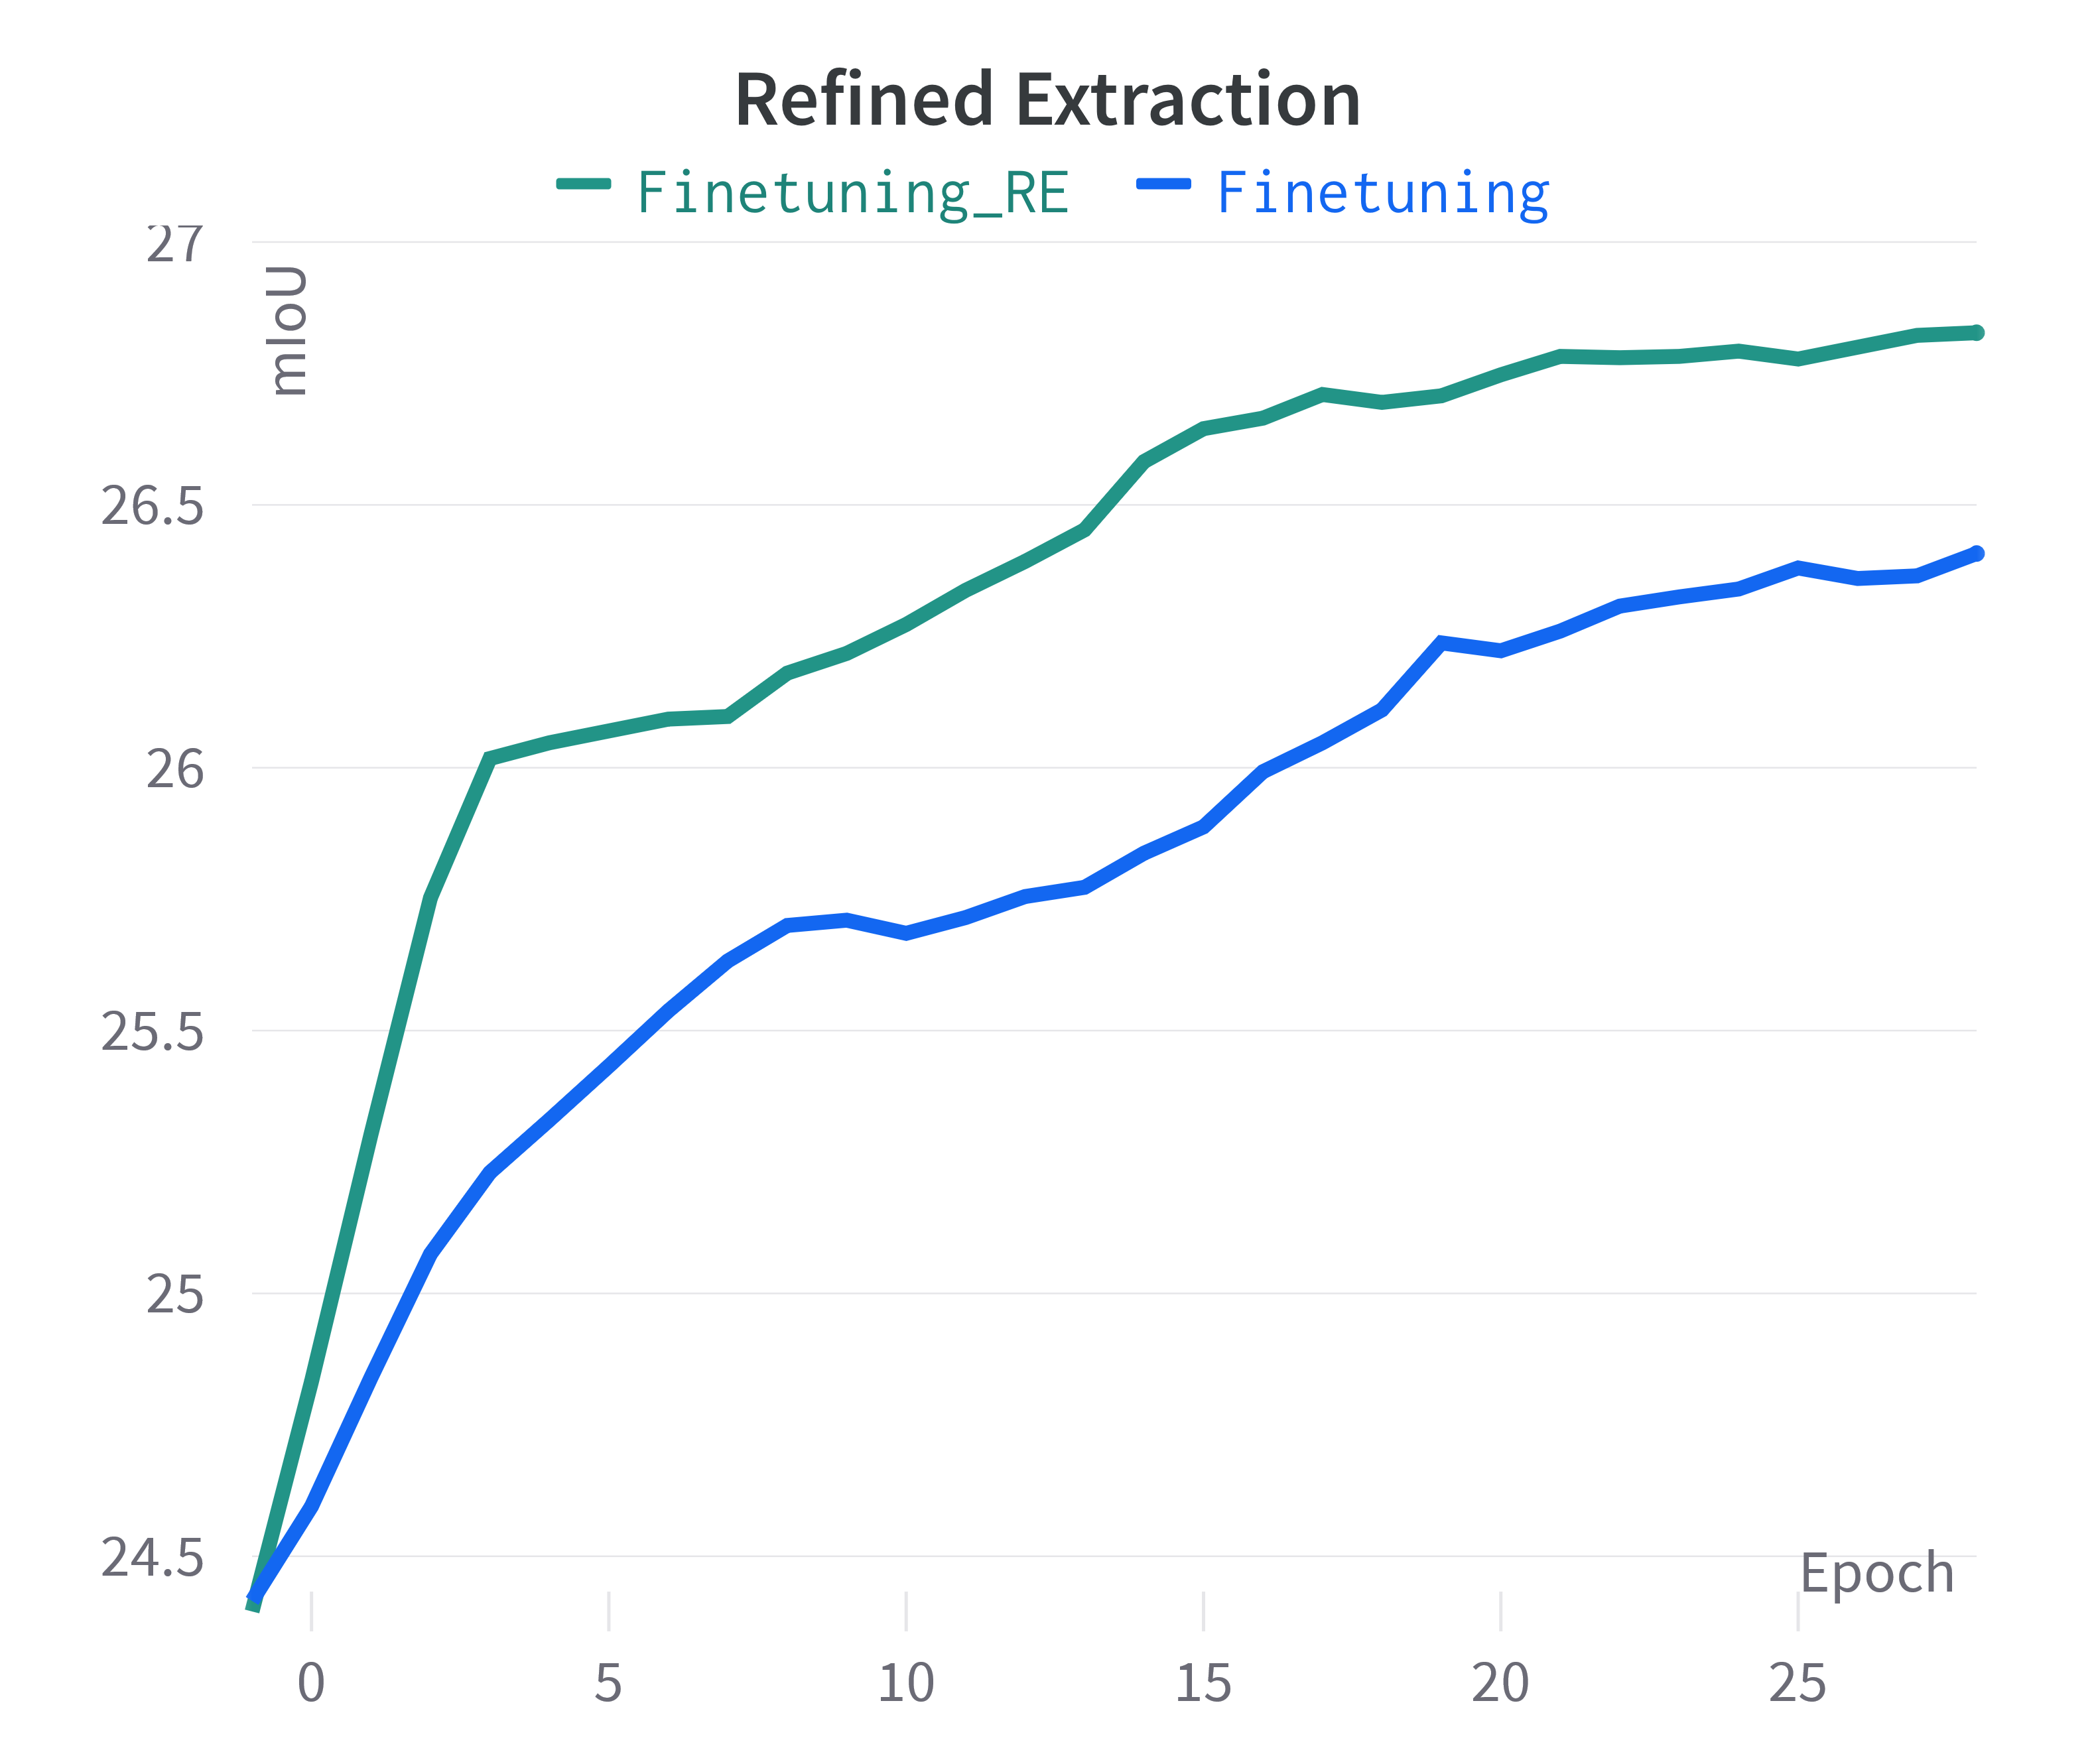
\includegraphics[scale=0.13]{figures/experiments/plots/refinedextraction.png}}
    \caption[Refined Text Extraction]{}
    % \caption[Ablation Study on Number of Stages]{\textbf{Ablation Study on Number of Stages}}
    \label{fig:pcaclasses}
\end{centering}
\end{figure}
%\section{Refinement in Label Extraction}
%\label{sec:ftre}
%For multi-label loss, GroupViT extracts a defined number of nouns or noun phrases from the caption. However, when the number of extracted labels fall short of this defined count, we address this by duplicating the caption. This ensures that the required number of labels is reached, maintaining consistent input lengths across all instances. To enhance clarity and reduce noise, we propose to substitute the caption with the <PAD> token. As <PAD> tokens are primarily introduced to ensure uniform input length, their embeddings are devoid of meaningful content. Therefore, we suggest assigning null values to their embeddings, encouraging the model to focus exclusively on pertinent input information and minimizing bias introduced by padding tokens. Our experiments, spanning over 30 epochs, reveals an improvement in performance, as indicated in Table \ref{tab:refinedextraction}. This discovery motivates us to adopt the practice of embedding <PAD> tokens with void embeddings. We provide a qualitative analysis of this baseline on PASCAL VOC in Fig. \ref{fig:qualitative_refined}
%% \begin{table}[htbp]
% \begin{center}
%     \begin{tabular}{|c|c|c|}
%         \hline
%         Model &  Data & mIoU     \\ \hline
%         \gvit & \pvoc & $52.29$  \\
%         \gvit & \coco & $24.3$   \\
%         \ovs  & \pvoc & $53.78$  \\
%         \ovs  & \coco & $25.06$  \\
%         \hline
%     \end{tabular}
%     \end{center}

%     \caption[Table caption]{\textbf{Table caption.} foo bar...\\}
%     \label{tab:accuracy}
% \end{table}




% \begin{table}[htbp]
%   \centering
%   \caption{GroupViT vs OVSegmentator}
%   \begin{tabular}{ccc|l|l|l}
%     \toprule
%     Model & Finetuned & \multicolumn{4}{c}{Datasets} \\
%     %\cmidrule(lr){1-2} \cmidrule(lr){3-4}
%     & components& VOC & COCO & ADE20K & Context\\
%     \midrule
%     \gvit(Original) &  & 52.29 & 24.3 \\
%     \gvit & GB  & 50.16 & 26.26 \\
%     \gvit & VE & 45.46 & 21.44 \\
%     \gvit(NPE) & GB & 50.45 & 26.78 \\
%     \ovs  & GB + MMD & 53.78 & 25.06 \\
%     \bottomrule
%   \end{tabular}
% \end{table}



\begin{table}[htbp]
  \centering
  \begin{tabular}{c|c|c|l|l|l}
    \toprule
    \multirow{2}{*}{Model} & \multirow{2}{*}{Method} & \multicolumn{4}{c}{Datasets} \\
    %\cmidrule(lr){1-2} \cmidrule(lr){3-4}
    \cline{3-6}
    &  & COCO & PVOC & PContext & ADE20K \\
     
    \midrule
    \gvit & Original & 24.3 & 52.29  & 22.39 & 8.56\\
    \midrule
    \gvit & Fine-tuning & 25.64  & 48.26 & 21.33 & \textbf{7.64}\\
    %\gvit & VE& 45.46 & 21.44 \\
    \midrule
    \gvit & \textbf{Fine-tuning} & \textbf{26.2} & \textbf{49.37} & \textbf{21.88} & 7.61 \\
      & \textbf{with refined extraction} &  &  && \\
    %\ovs  & GB + MMD & 53.78 & 25.06 \\
    \bottomrule
  \end{tabular}
  \caption[\textbf{Fine-tuning with Refined Extraction of Labels}]{\textbf{Fine-tuning with Refined Extraction of Labels.} We compare vanilla fine-tuning with the model trained with refined label extraction methodology. We also provide mIoU score of the pretrained model for reference.}
  \label{tab:refinedextraction}
\end{table}

\begin{table}[htbp]
  \centering
  \begin{tabular}{c|c|c|l|l|l}
    \toprule
    \multirow{2}{*}{Model} & \multirow{2}{*}{Method} & \multicolumn{4}{c}{Datasets} \\
    %\cmidrule(lr){1-2} \cmidrule(lr){3-4}
    \cline{3-6}
    &  & COCO & PVOC & PContext & ADE20K \\
     
    \midrule
    \multirow{4}{*}{\gvit} & {\color{gray}Original} & {\color{gray}24.3} & {\color{gray}52.29}  & {\color{gray}22.39} & {\color{gray}8.56}\\
    \cmidrule{2-6}
     & Fine-tuning & 25.64  & 48.26 & 21.33 & \textbf{7.64}\\
    %\gvit & VE& 45.46 & 21.44 \\
    \cmidrule{2-6}
     & Fine-tuning & \textbf{26.2} & \textbf{49.37} & \textbf{21.88} & 7.61 \\
      & with Refined Text Set &  &  && \\
    %\ovs  & GB + MMD & 53.78 & 25.06 \\
    \bottomrule
  \end{tabular}
  \caption[\textbf{Fine-tuning with Refined Extraction of Labels}]{\textbf{Fine-tuning with Refined Extraction of Labels.} We compare vanilla fine-tuning with the model trained with refined label extraction methodology. We also provide mIoU score of the pretrained model for reference.}
  \label{tab:refinedextraction}
\end{table}




% \begin{table}[htbp]
%   \centering
%   \caption{GroupViT - Impact of curated labels }
%   \begin{tabular}{ccc|l}
%     \toprule
%     Model & Method & \multicolumn{2}{c}{Datasets} \\
%     \cmidrule(lr){1-2} \cmidrule(lr){3-4}
%     & &\coco & \pvoc \\
%     \midrule
%     \gvit & All entities & 25.76 \\
%     \gvit & Entity\_freq$>=1K$ & 25.63 \\
%     \gvit & Entity\_freq$>=5K$ & 24.83 \\
%     \bottomrule
%   \end{tabular}
% \end{table}


% \documentclass{article}
% \usepackage{booktabs}

% \begin{document}

% \begin{table}[htbp]
%   \centering
%   \caption{My Pretty Table}
%   \begin{tabular}{ccc}
%     \toprule
%     Column 1 & Column 2 & Column 3 \\
%     \midrule
%     Row 1, Cell 1 & Row 1, Cell 2 & Row 1, Cell 3 \\
%     Row 2, Cell 1 & Row 2, Cell 2 & Row 2, Cell 3 \\
%     Row 3, Cell 1 & Row 3, Cell 2 & Row 3, Cell 3 \\
%     \bottomrule
%   \end{tabular}
% \end{table}

% \end{document}
%
%\begin{figure}[t]
%  %   \begin{tabular}{ccccc}
%  %   \textbf{Image} & \textbf{Column 2} & \textbf{Column 3} & \textbf{Column 4} &    \textbf{Ground Truth}\\
%  % \end{tabular}
%  \centering
%
%  \vspace{-0.5em}
% 
%  \subfloat {\textbf{\small \ \ Image}}
%  \hspace{4em}
%  \subfloat {\textbf{\small \ \ \ \ \ \ Pretrained}}
%  \hspace{4em}
%  \subfloat {\textbf{\small \ \ Fine-tuned}}
%  \hspace{2em}
%  \subfloat {\textbf{\small \ \ Ground-Truth}}
%  \vspace{-0.05em} 
%  \vspace{-0.05em} 
%  {\includegraphics[width=0.24\textwidth]{figures/experiments/pascal/0000.jpg}}
%  {
\includegraphics[width=0.24\textwidth]{figures/experiments/pascal/orgckpt/0000.png}}
%  {
\includegraphics[width=0.24\textwidth]{figures/experiments/pascal/ft/0000.png}}
%  {
\includegraphics[width=0.24\textwidth]{figures/experiments/pascal/gt/2007_000033.png}}
%  
%  {\includegraphics[width=0.24\textwidth]{figures/experiments/pascal/0010.jpg}}
%  {
\includegraphics[width=0.24\textwidth]{figures/experiments/pascal/orgckpt/0010.png}}
%  {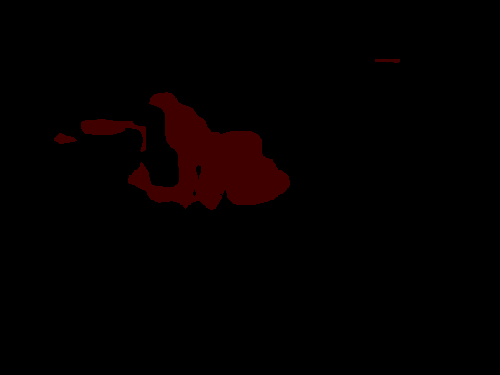
\includegraphics[width=0.24\textwidth]{figures/experiments/pascal/ft/0010.png}}
%  {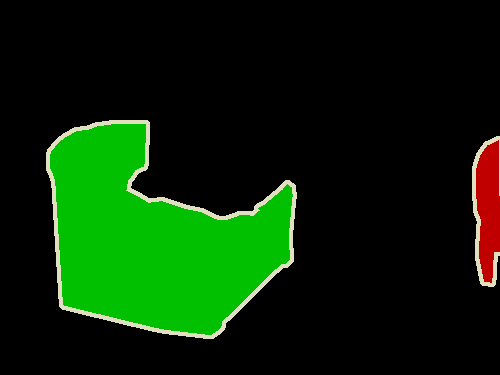
\includegraphics[width=0.24\textwidth]{figures/experiments/pascal/gt/2007_000452.png}}
%  
%  {\includegraphics[width=0.24\textwidth]{figures/experiments/pascal/0013.jpg}}
%  {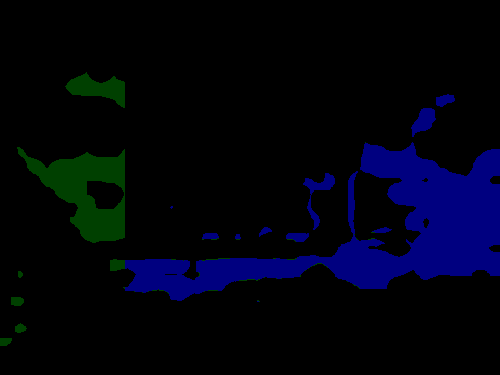
\includegraphics[width=0.24\textwidth]{figures/experiments/pascal/orgckpt/0013.png}}
%  {
\includegraphics[width=0.24\textwidth]{figures/experiments/pascal/ft/0013.png}}
%  {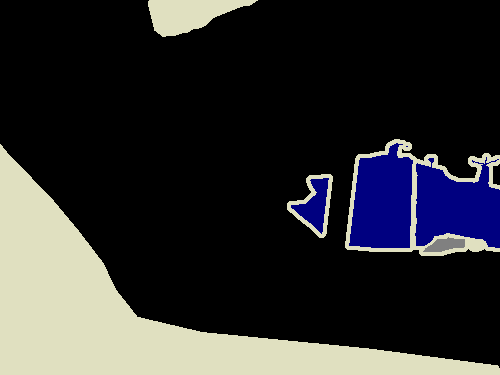
\includegraphics[width=0.24\textwidth]{figures/experiments/pascal/gt/2007_000529.png}}
%
%  {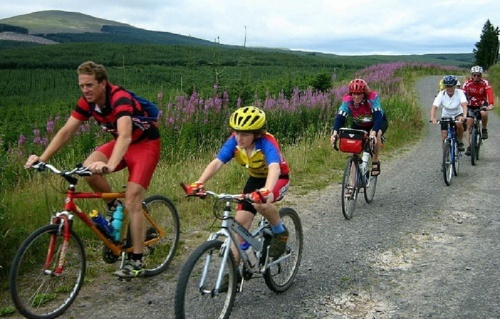
\includegraphics[width=0.24\textwidth]{figures/experiments/pascal/image/0039.jpg}}
%  {
\includegraphics[width=0.24\textwidth]{figures/experiments/pascal/orgckpt/0039.png}}
%  {
\includegraphics[width=0.24\textwidth]{figures/experiments/pascal/ft/0039.png}}
%  {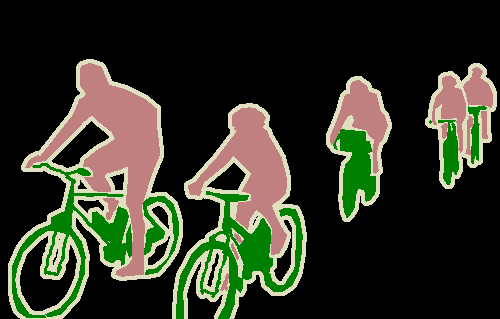
\includegraphics[width=0.24\textwidth]{figures/experiments/pascal/gt/2007_001311.png}}
%\caption[\textbf{Qualitative Analysis after Fine-tuning on Pascal VOC}]{\textbf{Qualitative Analysis after Fine-tuning GroupViT on Pascal VOC}}
%\label{fig:qualitative_refined}
%
%\end{figure}
%
%
%\subsection{Extract Labels with Most Frequent Entities}
%
%In our text augmentation process, detailed in Section \ref{sec:text_aug}, we extract nouns from caption using NLTK. It is often observed that NLTK  misidentifies nouns and extracts words like `twice', `exact', `Jonas', `TYPING', etc., despite our focus on Nouns (`NN'), Plural Nouns (`NNS'), and Proper Nouns (`NNP'). It is important to note that NLTK tags such as `NN', `NNS', and `NNP' serve as the basis for GroupViT's noun extraction from captions.\\
%For our next set of experiments, we extract all nouns and their frequencies from the MSCOCO training dataset, resulting in 27,089 nouns. We observe that a substantial number of these nouns lacked clear entity representation. To address this, we choose two sets: one with nouns appearing more than 1000 times (383 nouns) in the entire training dataset, and another with frequencies exceeding 5000 (88 nouns). Our intention was to create cleaner label sets that would offer a more precise entity representation.\\
%During training, we extract nouns and retain those belonging to the selected noun sets. If the count of retained nouns fall below the desired number of labels, we resort to using other nouns extracted from captions using the NLTK library, following the standard procedure. \\
%Intriguingly, we observe that the model exhibits better performance with the conventional extraction method. Our speculation revolves around the idea that selecting nouns based on their frequency might overly focus the model on a narrow selection of entities, hampering its ability to learn other entities or their synonyms.\\
%The results of our experiments utilizing the curated set of nouns with frequencies exceeding 1000 and 5000 were shown in Table \ref{tab:curatedlabels}. However, since we do not observe significant performance improvements and witness less promising performance during the initial epochs, we restrict the model training to the initial 5 epochs.
%% \begin{table}[htbp]
%   \centering

%   \begin{tabular}{ccc}
%     \toprule
%     Model & Method & COCO \\
%     \midrule
%     \gvit & All entities & 25.76 \\
%     \gvit & Entity\_freq$>=1K$ & 25.25 \\
%     \gvit & Entity\_freq$>=5K$ & 23.86 \\
%     \bottomrule
%   \end{tabular}
%   \caption[\textbf{Impact of curated labels}]{\textbf{Impact of curated labels }}
%  \label{tab:curatedlabels}
% \end{table}
\begin{table}[htbp]
  \centering
  \begin{tabular}{c|c|c|l|l|l}
    \toprule
    \multirow{2}{*}{Model} & \multirow{2}{*}{Method} & \multicolumn{4}{c}{Datasets} \\
    %\cmidrule(lr){1-2} \cmidrule(lr){3-4}
    \cline{3-6}
    &  & COCO & PVOC & PContext & ADE20K \\
    \midrule
    \gvit & All Entities & \textbf{25.76} & \textbf{49.20} & \textbf{21.87} & \textbf{7.50}\\
    %\gvit & VE& 45.46 & 21.44 \\
    \midrule
    
    \gvit &  Entity\_freq$>=1K$ & 25.25   & 48.70 & 21.72 & 6.95\\
    \midrule
    
    \gvit &  Entity\_freq$>=5K$ & 23.86  & 46.87 & 21.19 & 6.63\\
    %\ovs  & GB + MMD & 53.78 & 25.06 \\
    \bottomrule
  \end{tabular}
   \caption[\textbf{Impact of Curated Labels}]
   {\textbf{Impact of Curated Labels.} We assess the impact of curated labels by comparing the mIoU scores of three models: one trained with labels having frequencies over 1K in the COCO Caption dataset (`Entity\_freq$\geq1$K'), another with labels having frequencies over 5K (`Entity\_freq$\geq5$K'), and the vanilla model, which includes all entities.}
   % {Here, we compare mIoU score of model trained with labels with high frequencies in the training dataset with the vanilla model. Model ` Entity\_freq$>=1K$' prioritise labels having frequency over 1K in the COCO Caption dataset while extracting labels from caption.  Model ` Entity\_freq$>=5K$' prioritise labels having frequency over 5K. Model 'All Entities' is the vanilla mdoel }
 \label{tab:curatedlabels}
\end{table}
%\begin{figure}[t]
%\centering
%\begin{subfigure}{0.3\textwidth}
%    \centering
%    \includegraphics[width=\linewidth]{figures/experiments/entropymaps/finetuned/13/0013.jpg}
%\end{subfigure}
%\begin{subfigure}{0.3\textwidth}
%    \centering
%    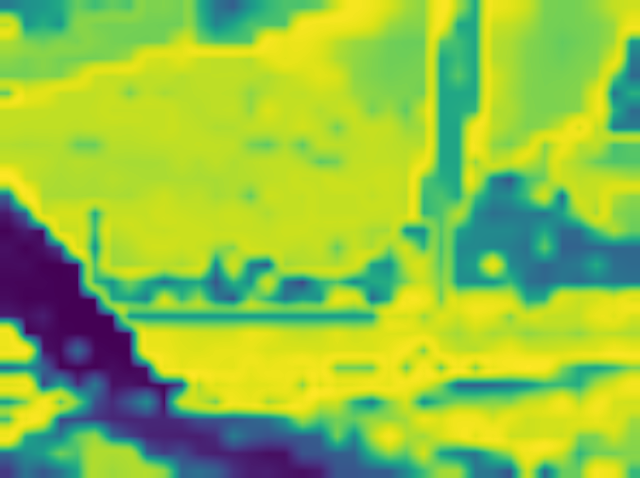
\includegraphics[width=\linewidth]{figures/experiments/entropymaps/finetuned/13/entropy_mapwithoutcb.png}
%\end{subfigure}
%\begin{subfigure}{0.3\textwidth}
%\label{fig:postregentropy}
%    \centering
%    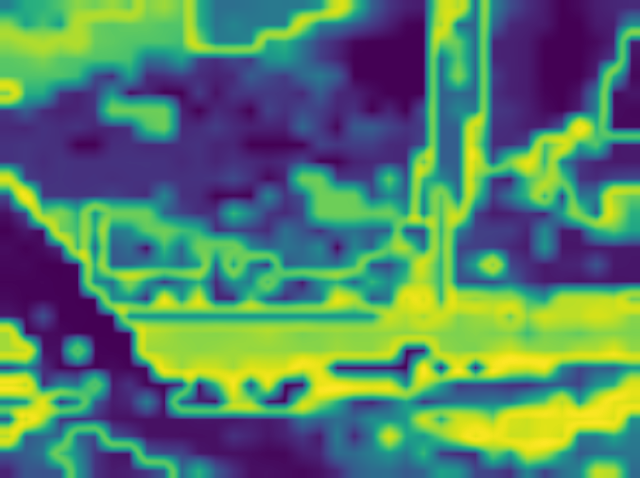
\includegraphics[width=\linewidth]{figures/experiments/entropymaps/er/13/entropy_mapwithoutcb.png}
%\end{subfigure}
%\begin{subfigure}{0.3\textwidth}
%    \centering
%    \includegraphics[width=\linewidth]{figures/experiments/entropymaps/finetuned/10/0010.jpg}
%\end{subfigure}
%\begin{subfigure}{0.3\textwidth}
%    \centering
%    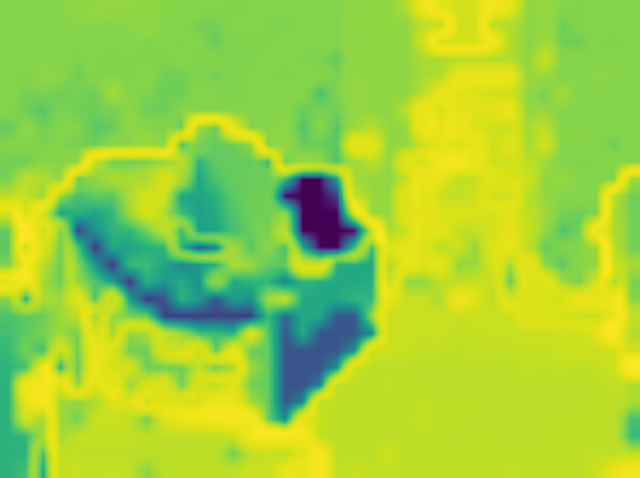
\includegraphics[width=\linewidth]{figures/experiments/entropymaps/finetuned/10/entropy_mapwithoutcb.png}
%\end{subfigure}
%\begin{subfigure}{0.3\textwidth}
%    \centering
%    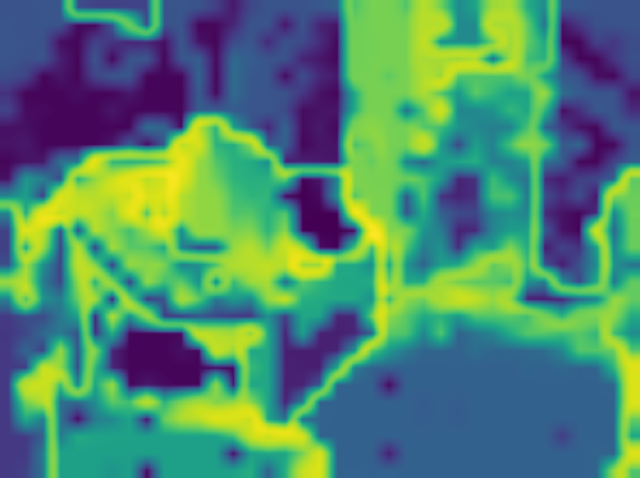
\includegraphics[width=\linewidth]{figures/experiments/entropymaps/er/10/entropy_mapwithoutcb.png}
%\end{subfigure}
%\caption[\textbf{Visualization of Entropy Distribution}]{\textbf{Visualization of Entropy Distribution:} Left - Image. Center - Entropy of Patch tokens over Group Tokens: Pre-regularization. Right - Entropy of Patch tokens over Group Tokens: Post-regularization.}
%\label{fig:groupser}
%\end{figure}
%
%\begin{figure}[t]
%\centering
%\begin{subfigure}{0.3\textwidth}
%    \centering
%    \includegraphics[width=\linewidth]{figures/experiments/entropymaps/finetuned/13/0013.jpg}
%\end{subfigure}
%\begin{subfigure}{0.3\textwidth}
%    \centering
%    \includegraphics[width=\linewidth]{figures/experiments/entropymaps/finetuned/13/class_entropywithoutcb.pdf}
%\end{subfigure}
%\begin{subfigure}{0.3\textwidth}
%    \centering
%    \includegraphics[width=\linewidth]{figures/experiments/entropymaps/er/13/class_entropywithoutcb.pdf}
%\end{subfigure}
%\begin{subfigure}{0.3\textwidth}
%    \centering
%    \includegraphics[width=\linewidth]{figures/experiments/entropymaps/finetuned/10/0010.jpg}
%\end{subfigure}
%\begin{subfigure}{0.3\textwidth}
%    \centering
%    \includegraphics[width=\linewidth]{figures/experiments/entropymaps/finetuned/10/class_entropywithoutcb.pdf}
%\end{subfigure}
%\begin{subfigure}{0.3\textwidth}
%    \centering
%    \includegraphics[width=\linewidth]{figures/experiments/entropymaps/er/10/class_entropywithoutcb.pdf}
%\end{subfigure}
%\caption[\textbf{Visualization of Entropy Distribution over Labels}]{\textbf{Visualization of Entropy Distribution over Labels:} Left - Image. Center - Entropy of Patch tokens over Labels: Pre-regularization. Right - Entropy of Patch tokens over Labels: Post-regularization.}
%\label{fig:labeler}
%\end{figure}
%
%
%\section{Entropy Regularization}
%\label{ref:er}
%
%We now employ entropy regularization penalties thoroughly discussed in Section \ref{sec:entropyreg}. We will conduct experiments with three penalties: (i) Penalty for Entropy over Groups, denoted as GE, detailed in Section \ref{sec:groupentropy}, (ii) Penalty for Entropy over extracted labels, denoted as LE, detailed in Section \ref{sec:LE}, (iii) Entropy over Groups and Labels in the `Segment Affinity Metric', denoted as SE, detailed in Section \ref{sec:tier}. Our experiments involve various combinations of these penalties as shown in Table \ref{tab:entropyreg}. Our findings indicate that all the regularization methods perform better than the last baseline reported in Table \ref{tab:refinedextraction}. Moreover, we observe that there is no advantage in using combination of regularization methods. Overall, `LE' outperforms rest of the methods with a slight margin. However, all these methods still falter on the downstream datasets. To further evaluate the efficacy of entropy regularization, we plan to test its impact at higher resolutions, as outlined in Section \ref{sec:hrcer}.
%
%
%\begin{table}[htbp]
  \centering
  \begin{tabular}{c|c|c|l|l|l}
    \toprule
    \multirow{2}{*}{Model} & \multirow{2}{*}{Method} & \multicolumn{4}{c}{Datasets} \\
    \cline{3-6}
    %\cmidrule(lr){1-2} \cmidrule(lr){3-4}
    & & COCO & PVOC & PContext & ADE20K\\
    \midrule
    \gvit & Original & 24.3 & \textbf{52.29} & 22.39 & \textbf{8.56}\\
    \midrule
    \gvit & Fine-tuned(RE) & 26.2 & 49.37 & 21.88 & 7.61 \\
    \midrule
    \gvit & SE  & 26.61 & 48.78 & 21.61 & 7.54\\
    \midrule
    \gvit & LE  & \textbf{26.76} & 49.69 & 21.92 & 7.53 \\
    \midrule
    \gvit & GE   & 26.61 & 50.16 & 22.41 & 7.82 \\
    \midrule
    \gvit  & GE + SE  & 26.41 & 50.92 & 22.65 & 7.51\\
    \midrule
    \gvit  & LE + SE  & 26.61 & 49.77 & 21.8 & 7.32 \\
    \midrule
    \gvit  & GE + LE  & 26.66 & 51.41 & \textbf{22.67} & 7.67\\
    \midrule
    \gvit  & GE + LE + SE  & 26.61 & 50.67 & 22.47 & 7.72\\
    \bottomrule
  \end{tabular}
   \caption[\textbf{Entropy Regularization}]{\textbf{Entropy Regularization}. Here, first row represents the original checkpoint. Fine-tuned(RE) refers to model fine-tuned with refined label extraction methodology. GE, SE and LE indicates models trained with penalty for entropy over groups, entropy over segment affinity metric,  and entropy over labels respectively. `+' between them indicates model is trained with more than one loss function.}
   
\label{tab:entropyreg}
\end{table}

% \begin{table}[t]
%     \scriptsize
%     \centering
%     \caption{Assessment of Approaches}
%     \label{tab:multi_shape}
%     \setlength\tabcolsep{5.0pt}
%     \begin{threeparttable}
%         \begin{tabular}{c|c|c|c|c|c|c|c}
%             \toprule
%                 % \multirow{2}{2.0cm}{GroupViT} &  \multirow{2}{1.5cm}{\centering GE} &\multirow{2}{1.5cm}{\centering LE}&\multirow{2}{1.5cm}{\centering SE} &\multicolumn{4}{c}{Datasets} \\
%                 % %\cmidrule(lr){1-2} \cmidrule(lr){3-4}        
%                 % \cline{5-8}
%                 % & &  &   & COCO & PVOC & PContext & ADE20K \\
%                 GroupViT &  GE &  LE &  SE & COCO} \\
%                 %\cmidrule(lr){1-2} \cmidrule(lr){3-4}        

%                 \midrule
%                 %single shape + sum & 65 & 70 & 68 \\
%                  Original & - & - & - &  24.3  & \textbf{52.29} & 22.39 &  \textbf{8.59} \\
%                 \midrule
%                 \multirow{8}{*}{Fine-tuned (RTE)} & - & - & - & 26.2 & 49.37 & 21.88 & 7.61 \\
%                 \cmidrule{2-8}
%                 %GE
%                  & \checkmark & - & - & 26.61 & 50.16 & 22.41 & 7.82 \\
%                  %LE
%                  \cmidrule{2-8}
%                  & - & \checkmark  & - & \textbf{26.76} & 49.69 & 21.92 & 7.53 \\
%                 %SE
%                 \cmidrule{2-8}
%                  & - & - & \checkmark  & 26.61 & 48.78 & 21.61 & 7.54 \\
%                 %\midrule
%                 %GE+LE
%                 \cmidrule{2-8}
%                   & \checkmark & \checkmark & - & 26.66 & 51.41 & \textbf{22.67} & 7.67\\
%                 %GE+SE
%                 \cmidrule{2-8}
%                   & \checkmark & - & \checkmark & 26.41 & 50.92 & 22.65 & 7.51\\
%                 %LE+SE
%                 \cmidrule{2-8}
%                   & - & \checkmark & \checkmark & 26.61 & 49.77 & 21.8 & 7.32\\
%                 %\midrule
%                 %both + goal + sum  & 65 & 75 & 70\\
%                 %GE+LE+SE
%                 \cmidrule{2-8}
%                  & \checkmark & \checkmark & \checkmark & 26.61 & 50.67 & 22.47 & 7.72\\
%                 \bottomrule
%         \end{tabular}
%     \footnotesize
%     \vspace{.3em}
%     \hspace{-.11\linewidth}

%     \end{threeparttable}
%     \vspace{-0.3cm}
% \end{table}



%
%\section{Fine-tuning on High Resolution}
%Dosovitskiy et al. propose fine-tuning Vision Transformers (ViT) at a higher resolution than the resolution used in pre-training\cite{dosovitskiy2020image}. This approach has demonstrated enhanced model performance, highlighting resolution's role in fine-tuning strategies. Therefore, we adopt a higher resolution of 384, deviating from the standard 224, for our following experiments.\\
%To achieve this, we utilize positional encoding interpolation, similar to ViT\cite{dosovitskiy2020image}. Specifically, we employ bicubic interpolation to resize the positional encoding loaded from the pretrained model to the new dimension. Subsequently, we rearrange the tensor to match the expected format within the model and update the positional encoding parameter in the model's state dictionary with the appropriately resized positional encoding.\\ 
%We present our findings in Table \ref{tab:highres}.
%Our experimentation unveiled a noteworthy insight: fine-tuning the model with an image resolution of 384 improved the training process. However, this improvement came at the expense of compromised performance on downstream datasets.
%\begin{figure}[t]
%  \centering
%  % \subfloat {\textbf{\footnotesize \ \ \ \ \  \ \ \ Image}}
%  % \hfill
%  % \subfloat {\textbf{\footnotesize Finetune}}
%  % \hfill
%  % \subfloat {\textbf{\footnotesize New Baseline}}
%  % \hfill
%  % \subfloat {\textbf{\footnotesize Ground-Truth}}
%  
%  % \vspace{-0.05em}
%  
%  \vspace{-0.5em}
% 
%  \subfloat {\textbf{\small \ \ \ \ Image}}
%  \hspace{4em}
%  \subfloat {\textbf{\small \ \ \  Fine-tuned}}
%  \hspace{4em}
%  \subfloat {\textbf{\small New Baseline}}
%  \hspace{2em}
%  \subfloat {\textbf{\small Ground-Truth}}
%  \vspace{-0.05em} 
%  {\includegraphics[width=0.24\textwidth]{figures/experiments/pascal/0000.jpg}}
%  {\includegraphics[width=0.24\textwidth]{figures/experiments/pascal/ft/0000.png}}
%  {\includegraphics[width=0.24\textwidth]{figures/experiments/pascal/highres+ge/0000.png}}
%  {\includegraphics[width=0.24\textwidth]{figures/experiments/pascal/gt/2007_000033.png}}
%  
%  {\includegraphics[width=0.24\textwidth]{figures/experiments/pascal/0010.jpg}}
%  {\includegraphics[width=0.24\textwidth]{figures/experiments/pascal/ft/0010.png}}
%  {\includegraphics[width=0.24\textwidth]{figures/experiments/pascal/highres+ge/0010.png}}
%  {\includegraphics[width=0.24\textwidth]{figures/experiments/pascal/gt/2007_000452.png}}
%  
%  {\includegraphics[width=0.24\textwidth]{figures/experiments/pascal/0013.jpg}}
%  {\includegraphics[width=0.24\textwidth]{figures/experiments/pascal/ft/0013.png}}
%  {\includegraphics[width=0.24\textwidth]{figures/experiments/pascal/highres+ge/0013.png}}
%  {\includegraphics[width=0.24\textwidth]{figures/experiments/pascal/gt/2007_000529.png}}
%
%  {\includegraphics[width=0.24\textwidth]{figures/experiments/pascal/image/0039.jpg}}
%  {\includegraphics[width=0.24\textwidth]{figures/experiments/pascal/ft/0039.png}}
%  {\includegraphics[width=0.24\textwidth]{figures/experiments/pascal/highres+ge/0039.png}}
%  {\includegraphics[width=0.24\textwidth]{figures/experiments/pascal/gt/2007_001311.png}}
%\caption[\textbf{Qualitative Analysis on Pascal VOC for model trained with Entropy Regularization}]{\textbf{Qualitative Analysis on Pascal VOC for model trained with Entropy Regularization on a higher resolution of 384}}
%\label{fig:qualitative_hrge}
%\end{figure}
%
%
%\subsection{High Resolution Complements Entropy Regularization}
%\label{sec:hrcer}
%Continuing our investigation, we explore higher resolution training with entropy regularization. For this, we use group entropy loss (GE), label entropy loss(LE) and penalty for entropy over segment affinity metric(SE). We present our findings in Table \ref{tab:highres} which shows improved performance for `GE' on COCO as well as on PASCAL VOC while performance on PASCAL Context and ADE20K remain steady. We observe some improvements for `LE' and `SE' on COCO but these methods still falter on the downstream datasets. \\
%We also provide visualizations of entropy changes over groups and labels, depicted in Fig. \ref{fig:groupser} and \ref{fig:labeler}, both pre- and post-regularization for two images from PASCAL VOC. Figure \ref{fig:groupser} highlights a significant reduction in pixel entropy over groups post-regularization for both the images. Conversely, in Fig. \ref{fig:labeler}, we observe improvements in the top row but limited changes in the bottom row. This aligns with our observation that employing `GE' is more beneficial than `LE' specifically on downstream datasets. These samples can also be visualized in qualitative examples in Fig. \ref{fig:qualitative_hrge} \\
%We note that training at 384 resolution increases resource requirements: an epoch takes about 7 more minutes than at 224 resolution, translating to 3.5 hours for 30 epochs. However, as visualized in Fig. \ref{fig:plot_hr_ger}, the model shows significant speedup over previous baselines.
%In summary, fine-tuning on a higher resolution of 384 with entropy regularization improves the performance without impacting performance on the downstream datasets.
%
\begin{table}[htbp]
  \centering
  \begin{tabular}{c|c|c|l|l|l}
    \toprule
    % Method & Training Res. & \multicolumn{4}{c}{Datasets} \\
    % %\cmidrule(lr){1-2} \cmidrule(lr){3-4}
    % &  & COCO & VOC & Context & ADE20K\\
    % \midrule
    \multirow{2}{*}{Method} & Training & \multicolumn{4}{c}{Datasets} \\
    %\cmidrule(lr){1-2} \cmidrule(lr){3-4}
        
    \cline{3-6}
    & Resolution & COCO & PVOC & PContext & ADE20K \\

    \midrule
    Original & 224 & 24.3 & 52.29  & \textbf{22.39} & \textbf{8.56}\\
    \midrule
    Fine-tuned & 384  & 26.81 & 46.9 & 20.82 & 7.77\\
    \midrule
    %GE+LE &  384  & \textbf{28.13} & 53.29 & \textbf{22.4} & 7.66 \\
    %GE+LE(50) & 384  & 53.38  & 28.25  & \textbf{22.45}  & 7.69 \\
    SE  & 384  & 27.24 & 49.54 & 21.61 & 7.74 \\
    \midrule
    LE  & 384  & 27.25 & 49.46 & 21.87 & 7.74 \\
    \midrule
    GE  & 384  & \textbf{27.86} & \textbf{53.38}& 22.25 & 7.66 \\
    %GE(50) & 384 & \textbf{53.49} & \textbf{28.3} & 22.33  & 7.77 \\
    \bottomrule
  \end{tabular}
  \caption[\textbf{High Resolution Fine-tuning}]{\textbf{High Resolution Fine-tuning}. Here, Fine-tuned is the model trained with refined extraction. GE is the model trained with group entropy loss. LE is trained with label entropy loss. SE is the model trained with penalty for entropy over the `segment affinity metric'.}
 \label{tab:highres}
\end{table}

%
%\section{Non-noisy Contrastive Loss}
%\label{sec:nncl}
%As described in Section \ref{sec:mll}, during the pretraining phase, GroupViT extracts labels from captions to create image-text pairs, which are then considered as positive instances within the multi-label loss formulation.  For fine-tuning, we use COCO, comprising just 600,000 data points, introducing a challenge.
%
%Specifically, there's a significant likelihood that same labels may appear across different images, potentially causing them to be misconstrued as negatives rather than their rightful status as positives.\\
%To address this, we extend our strategy to include identical labels from other images within the same mini-batch as positives. Notably, these same labels might have been prompted differently for other images. To address this, we check the labels in their original string representation. Additionally, comparison of labels in their string representation is more viable and less time-consuming than comparing embeddings. As a result, we avoid using a global batch to create the negative pool, which would require combining embeddings from mini-batches across all distributed systems.
%Consequently, this leads to a reduction in the number of negative pair available for comparison. Nonetheless, we observe a noteworthy trend: prioritizing the accuracy of positive pairs, even if it comes at the expense of negative pool, correlates with improved overall performance.\\
%Given the resource-intensive nature of this approach, we execute this experiment with a batch size of 128 across 4 machines, making a global batch size of 512. 
%We provide our findings in Table: \ref{tab:npe}. We observe superior performance of this approach on validation split of COCO and downstream datasets. We provide a qualitative analysis on COCO, PASCAL VOC and PASCAL Context in Fig. \ref{fig:qualitative_alldatabaseline}. Additionally, we provide exhaustive qualitative analysis on individual datasets in Section \ref{sec:qa}
%
%\begin{table}[htbp]
  \centering
  
  \begin{tabular}{c|c|c|l|l|l}
    \toprule
    \multirow{2}{*}{Model} & \multirow{2}{*}{Method} & \multicolumn{4}{c}{Datasets} \\
    %\cmidrule(lr){1-2} \cmidrule(lr){3-4}
        
    \cline{3-6}
    &  & COCO & PVOC & PContext & ADE20K \\

    \midrule
    %     \multirow{2}{*}{Model} & \multirow{2}{*}{\#labels} &\multirow{2}{*}{Text-Type}& \multicolumn{2}{c}{Datasets} \\
    % \cline{4-4}
    % \cline{5-5}
    %   % \cmidrule(lr){4-5}
    % & & & COCO & VOC\\
    % %\gvit & VE& 45.46 & 21.44 \\
    % \midrule
    
    \gvit & Original & 24.3  & 52.29 & 22.39 &  \textbf{8.59}\\
    \midrule
    \gvit & Fine-tuning &  26.81 &46.9 &  20.82 & 7.77\\
    \midrule
    \gvit & GE   & 27.86 & 53.38 & 22.25 & 7.66 \\
    \midrule
    \gvit & Non-noisy CL + GE &  \textbf{28.68}  & \textbf{53.41} & \textbf{23.34} & 7.96\\
    %\ovs  & GB + MMD & 53.78 & 25.06 \\
    \bottomrule
  \end{tabular}
  \caption[\textbf{Non-noisy Contrastive Loss}]{\textbf{Non-noisy Contrastive Loss.} Here, Fine-tuning is fine-tuning with refined extraction. GE denotes Group Entropy Regularization baseline. Non-noisy CL + GE denotes model trained with noise-free contrastive loss and Group Entropy Regularization. All the models are trained on the resolution of 384.}
  
\label{tab:npe}
\end{table}

% \begin{table}[t]
%     \scriptsize
%     \centering
%     \caption{Assessment of Approaches}
%     \label{tab:multi_shape}
%     \setlength\tabcolsep{5.0pt}
%     \begin{threeparttable}
%         \begin{tabular}{c|c|c|c|c|c|c|c}
%             \toprule
%                 \multirow{2}{2.0cm}{GroupViT} &  \multirow{2}{1.5cm}{\centering Refined Text Set} &\multirow{2}{1.5cm}{\centering Group Entropy}&\multirow{2}{1.5cm}{\centering Non-noisy CL} &\multicolumn{4}{c}{Datasets} \\
%                 %\cmidrule(lr){1-2} \cmidrule(lr){3-4}        
%                 \cline{5-8}
%                 & &  &   & COCO & PVOC & PContext & ADE20K \\

%                 \midrule
%                 %single shape + sum & 65 & 70 & 68 \\
%                  Original & - & - & - &  24.3  & 52.29 & 22.39 &  \textbf{8.59} \\
%                 \midrule
%                 \multirow{4}{*}{Fine-tuned} & - & - & - & 25.64  & 48.26 & 21.33 & 7.64 \\
%                  & \checkmark & - & - & 26.81 &46.9 &  20.82 & 7.77 \\
%                 %\midrule
%                   & \checkmark & \checkmark & - & 27.86 & 53.38 & 22.25 & 7.66\\
%                 %\midrule
%                 %both + goal + sum  & 65 & 75 & 70\\
%                  & \checkmark & \checkmark & \checkmark & \textbf{28.68}  & \textbf{53.41} & \textbf{23.34} & 7.96\\
%                 \bottomrule
%         \end{tabular}
%     \footnotesize
%     \vspace{.3em}
%     \hspace{-.11\linewidth}

%     \end{threeparttable}
%     \vspace{-0.3cm}
% \end{table}

%\newcommand{\incvisualsrow}[4]{
\begin{subfigure}{\linewidth}\begin{adjustbox}{width=\textwidth}{\def\arraystretch{0.2}\setlength\tabcolsep{#1pt}\begin{tabular}{ccccc}
\raisebox{1.2\normalbaselineskip}[0pt][0pt]{\rotatebox{90}{\tiny #2}} &
\includegraphics[height=2cm]{figures/experiments/coco/image/#3.jpg} &
\includegraphics[height=2cm]{figures/experiments/coco/orgckpt/#3.png} &
\includegraphics[height=2cm]{figures/experiments/coco/nonnoisy/#3.png} &
\includegraphics[height=2cm]{figures/experiments/coco/gt/#4.png} \\
\end{tabular}}\end{adjustbox}\end{subfigure}}

\newcommand{\incpascalvisualsrow}[4]{
\begin{subfigure}{\linewidth}\begin{adjustbox}{width=\textwidth}{\def\arraystretch{0.2}\setlength\tabcolsep{#1pt}\begin{tabular}{ccccc}
\raisebox{1.2\normalbaselineskip}[0pt][0pt]{\rotatebox{90}{\tiny #2}} &
\includegraphics[height=2cm]{figures/experiments/pascal/image/#3.jpg} &
\includegraphics[height=2cm]{figures/experiments/pascal/orgckpt/#3.png} &
\includegraphics[height=2cm]{figures/experiments/pascal/nonnoisybaseline/#3.png} &
\includegraphics[height=2cm]{figures/experiments/pascal/gt/#4.png} \\
\end{tabular}}\end{adjustbox}\end{subfigure}}

\newcommand{\inccontextvisualsrow}[4]{
\begin{subfigure}{\linewidth}\begin{adjustbox}{width=\textwidth}{\def\arraystretch{0.2}\setlength\tabcolsep{#1pt}\begin{tabular}{ccccc}
\raisebox{1.2\normalbaselineskip}[0pt][0pt]{\rotatebox{90}{\tiny #2}} &
\includegraphics[height=2cm]{figures/experiments/context/image/#3.jpg} &
\includegraphics[height=2cm]{figures/experiments/context/orgckpt/#3.png} &
\includegraphics[height=2cm]{figures/experiments/context/nonnoisy/#3.png} &
\includegraphics[height=2cm]{figures/experiments/context/gt/#4.png} \\
\end{tabular}}\end{adjustbox}\end{subfigure}}

\begin{figure}[thp]
\centering
  \vspace{-0.5em}
 
  \subfloat {\textbf{\small \ \ Image}}
  \hspace{4em}
  \subfloat {\textbf{\small \ \ \ Pretrained Model}}
  \hspace{1.5em}
  \subfloat {\textbf{\small Our Baseline}}
  \hspace{1.5em}
  \subfloat {\textbf{\small \ \ \ \ Ground-Truth}}
  \vspace{-0.02em} % Add some vertical space between rows
  \vspace{-0.05em}
\incvisualsrow{0.5}{\small \textbf{Coco}}{0013}{mask}
\incpascalvisualsrow{0.5}{\small \textbf{Pascal}}{0059}{2007_001763}
\inccontextvisualsrow{0.5}{\small \textbf{Context}}{0027}{2008_000084}
\incvisualsrow{0.5}{\small \textbf{Coco}}
{0021}{000000001993_instanceTrainIds}
\incpascalvisualsrow{0.5}{\small \textbf{Pascal}}{0039}{2007_001311}
\inccontextvisualsrow{0.5}{\textbf{Context}}{0018}{2008_000062}


\caption[\textbf{Qualitative analysis of the baseline across datasets}]{\textbf{Qualitative analysis of the baseline across datasets}. We visualize segmentation maps obtained from PASCAL VOC, COCO and PASCAL Context for the model trained with noise-free contrastive loss as reported in Table \ref{tab:npe}.}
\label{fig:qualitative_alldatabaseline}
\end{figure}

  
%
%
%\section{Impact of Inference Settings}
%\label{sec:infsettings}
%
%Next, we analyze how inference parameters like resolution and background threshold influence the result. We explore impact of inference resolution and background threshold. The background threshold influences background pixel recognition: lower values enhance foreground coverage, while higher values require more confidence for foreground assignment. This parameter's tuning balances false positives and negatives, refining segmentation accuracy. Our results are in Table \ref{tab:infhp}, where we show that for COCO a resolution of 512 with a background threshold of 0.95 works better than other settings. However, for \pvoc, a really high threshold of 0.99 works the best.
%
%
%
%\begin{table}[htbp]
  \centering
  \begin{tabular}{c|c|c|c|l}
    \toprule
    % Model  & Inf Res & Bg Thresh & \multicolumn{2}{c}{Datasets} \\
    % \cmidrule(lr){1-4} \cmidrule(lr){4-5}
    % & & & COCO & VOC \\
     \multirow{2}{*}{Model} & \multirow{2}{*}{Inference Res} &\multirow{2}{*}{Bg Threshold}& \multicolumn{2}{c}{Datasets} \\
    \cline{4-4}
    \cline{5-5}
      % \cmidrule(lr){4-5}
    & & & COCO & PVOC\\
    \midrule
    \gvit & 448  & 0.9 & 28.68 & 52.03 \\
    \midrule
    \gvit & 448 & 0.95 & 28.71 & 53.41 \\
    \midrule
    \gvit & 448  & 0.98 & 28.44 & 54.89 \\
    \midrule
    \gvit & 448  & 0.99 & 28.43 & 55.07 \\
    \midrule
    \gvit & 512  & 0.9 & 28.61 & 53.05 \\
    \midrule
    \gvit & 512  & 0.95 & \textbf{28.96} & 54.21 \\
    \midrule
    \gvit & 512  & 0.98 & 28.9 & 55.31 \\
    \midrule
    \gvit & 512  & 0.99 & 28.89 & \textbf{56.41} \\
    \bottomrule
  \end{tabular}
  \caption[\textbf{Ablation on Inference Parameters}]{
  \textbf{Ablation on Inference Parameters.} Here, `Inference Res' represents resolution of images set during inference and `Bg Threshold' represents Background Threshold.
  }
\label{tab:infhp}
\end{table}

%% We further employ non-noisy contrastive loss for group entropy loss with training for images of higher potential as seen the potential bef
%% \begin{figure}[thp]
%%   \centering
%
%%   \begin{subfigure}{\linewidth}
%%     \centering
%%     \includegraphics[width=0.6\linewidth, height=0.4\textheight]{figures/fig_plots/ioupascal.png}
%%     \caption{\textbf{IoU Disparity per Class Compared to Pretrained Model on Pascal VOC Dataset}}
%%     \label{fig:pcaclasses}
%%   \end{subfigure}
%
%%   \begin{subfigure}{\linewidth}
%%     \centering
%%     \includegraphics[width=0.9\linewidth, height=0.58\textheight]{figures/fig_plots/ioucoco.png}
%%     \caption{\textbf{IoU Disparity per Class Compared to Pretrained Model on COCO Dataset.}We depict IoU differences for the 20 classes with positive and negative deviations from the pretrained model on COCO Dataset.}
%%     \label{fig:cocomiou}
%%   \end{subfigure}
%
%%   \caption{\textbf{IoU Disparity per Class Compared to Pretrained Models}}
%%   \label{fig:combined}
%% \end{figure}
%% First subfigure
%\begin{figure}[htb]
%  \centering
%  \includegraphics[width=0.9\linewidth, height=0.6\textheight]{figures/fig_plots/ioupascal.png}
%  \caption{\textbf{IoU Disparity per Class Compared to Pretrained Model on Pascal VOC Dataset}}
%  \label{fig:pcaclasses}
%\end{figure}
%
%% Second subfigure
%\begin{figure}[htb!]
%  \centering
%  \includegraphics[width=0.9\linewidth, height=0.6\textheight]{figures/fig_plots/ioucoco.png}
%  \caption[\textbf{IoU Disparity per Class Compared to Pretrained Model on COCO Dataset.}]{\textbf{IoU Disparity per Class Compared to Pretrained Model on COCO Dataset.} We depict IoU differences for the 20 classes with positive and negative deviations from the pretrained model on COCO Dataset.}
%  \label{fig:cocomiou}
%\end{figure}
%
%\section{Analysis of The Baseline}
%\subsection{Visualization of IoU Disparity}
%In this section, we delve into a comprehensive analysis of our baseline model, focusing on visualizing its impact on individual classes. To achieve this, we calculate the Intersection over Union (IoU) disparity across classes for the COCO dataset, as depicted in Figure \ref{fig:cocomiou}. Given the large number of classes, we present IoU disparity for the baseline against the pretrained model for a selection of 20 classes: the top-10 and bottom-10 ranked by IoU disparity.
%
%Our observations reveal interesting insights. Classes such as `bench', `scissors', and `sink' exhibit notably lower IoU compared to the pretrained model, with classes `person', `train', and `traffic light' also displaying diminishing performance. On the other hand, categories like `baseball glove' and several categories representing animal kingdom show significant improvement. To gain a deeper understanding, we offer a qualitative view of classes with low mIoU in Figure \ref{fig:cocobad}.
%
%In our qualitative analysis, we notice recurrent issues. For instance, `person' is frequently mislabeled as surrounding objects like `tie' or `baseball glove'. This trend is visible across various instances, illustrated in the initial rows of Figure \ref{fig:cocobad}. Additionally, over-masking tendencies arise in other classes like `traffic light' and `sink' where the model masks object and the associated structure together. Due to GroupViT's reliance on text-based weak supervision, the model struggles to attain pixel-level precision in segmentation. It tends to associate common object-related structures with the object itself, thus leading to lower mean IoU (mIoU) scores.
%
%After fine-tuning on MSCOCO, the model demonstrates improved performance on dataset-specific classes, such as `surfboard', `basketball glove', and `hotdog'. However, a recurrent issue persists — humans in the vicinity are occasionally mislabeled as these specific object classes due to their association with these items. This exemplifies the challenges arising from weak supervisory signals.
% 
%  
%Moving on to the Pascal VOC dataset (\pvoc), we proceed to compute the IoU disparity in relation to the pretrained model, visualized in Fig. \ref{fig:pcaclasses}. Notable enhancements emerge for classes like `aeroplane', `bicycle', `motorbike', `horse', and `sheep'. However, certain classes such as `person' and `plant' exhibit poorer performance. To gain deeper insights, we present a qualitative analysis of these classes in Figure \ref{fig:pascalbad}.
%
%Specifically, in the case of `plant' and `person', which show higher negative IoU disparity, we visually explore the reasoning through the initial rows of Figure \ref{fig:pascalbad}. When `plant' is in the foreground, the model performs well, yet it mislabels `trees' as `plant' in second row. Additionally, when `plant' is not the prominent object—as in the third row—it often remains unidentified. Similarly, the `person' mislabeling issue seen in COCO resurfaces here as well.
%
%In the context of other structures, such as `monitor' and `train', we observe over-masking tendencies. These structures tend to blend with their surroundings, resulting in the visualizations presented in Figure \ref{fig:pascalbad}.
%\begin{figure}[t]
%\centering
%
%\begin{subfigure}{\linewidth}
%    \includegraphics[width=\linewidth]{figures/fig_plots/tsne.pdf}
%    \caption[\textbf{Visualizations of learned representation space of Group Tokens for \pvoc}]{\textbf{Visualizations of learned representation space of Group Tokens for \pvoc} Left: features extracted from Group Tokens in pretrained model. Right: features extracted from Group Tokens in our baseline.}
%    \label{fig:voctsne}
%\end{subfigure}
%
%\begin{subfigure}{\linewidth}
%    \includegraphics[width=\linewidth]{figures/fig_plots/allfeat_tsne_plot_org_baseline_coco_lowmIoU.pdf}
%    \caption[\textbf{Visualizations of learned representation space of Group Tokens on COCO classes with low IoU}]{ \textbf{Visualizations of learned representation space of Group Tokens for COCO classes with low IoU}. Left: features extracted from Group Tokens in pretrained model. Right: features extracted from Group Tokens in our baseline.}
%    \label{fig:cocotsne}
%\end{subfigure}
%
%\caption{\textbf{Visualizations of Learned Representation Space }}
%\label{fig:feature_comparison}
%\end{figure}
%
%
%\subsection{Visualization of Representation Space}
%To visualize the representation spaces created by our baseline, we employ t-SNE\cite{van2008visualizing}, a dimensionality reduction technique. To achieve this, we utilize the validation splits of both  \pvoc and COCO datasets. We extract segment token features from the final stage that our baseline and pretrained model label with respective dataset categories.
%
%The outcomes are presented in Figure \ref{fig:voctsne} and Figure \ref{fig:cocotsne}. Given COCO's extensive class variety, we concentrate solely on classes with negative IoU disparity, as shown in Figure \ref{fig:cocomiou}. Our findings mirror those from the prior observations in Figure \ref{fig:cocomiou}.
%
%We note several trends for \pvoc. For the cluster of `plant', there's increased dispersion. Additionally, features corresponding to `person' often appear near clusters associated with `sofa' and `table'. The `monitor' cluster lacks clear demarcation from `chair' and `table'. Conversely, we observe improved clustering for `aeroplane', `motorbike', and `sheep' features. These observations reinforce our earlier insights in Figure \ref{fig:pcaclasses}.
%
%Our findings for COCO datasets also align with the insights from Figure \ref{fig:cocomiou}. We observe that the features corresponding to `bench' and `person' do not converge, indicating mislabeling. Further, our observation resonates with the depiction in Figure \ref{fig:cocobad}, second row, where features of `person' was identified as `tie'. Additionally, `scissors' and `vase' have only few features, suggesting that the model still needs improvement in identifying and grouping these classes. We hypothesize that these classes either frequently coexist with multiple objects or occupy relatively smaller visual areas. Once again, this underscores the challenge of achieving pixel-level accuracy due to the constraints of weak supervision, particularly in scenarios involving multiple objects within a single visual context.
%% \newcommand{\rulesep}{\unskip\ \vrule\ }


\begin{figure}[p!]
  \centering
  \subfloat {\textbf{\small \ \ Image}}
  \hspace{4em}
  \subfloat {\textbf{\small \ \ \ Pretrained Model}}
  \hspace{1.5em}
  \subfloat {\textbf{\small Our Baseline}}
  \hspace{1.5em}
  \subfloat {\textbf{\small \ \ \ \ Ground-Truth}}
  \vspace{-0.05em} % Add some vertical space between rows
  \vspace{-0.05em}
  

  {\includegraphics[width=0.24\textwidth, height=1.8cm]{figures/experiments/coco/image/0024.jpg}}
  {\includegraphics[width=0.24\textwidth, height=1.8cm]{figures/experiments/coco/orgckpt/0024.png}}
  {\includegraphics[width=0.24\textwidth, height=1.8cm]{figures/experiments/coco/nonnoisy/0024.png}}
  {\includegraphics[width=0.24\textwidth, height=1.8cm]{figures/experiments/coco/gt/000000002153_instanceTrainIds.png}}
  
  {\includegraphics[width=0.24\textwidth, height=1.8cm]{figures/experiments/coco/image/0042.jpg}}
  {\includegraphics[width=0.24\textwidth, height=1.8cm]{figures/experiments/coco/orgckpt/0042.png}}
  {\includegraphics[width=0.24\textwidth, height=1.8cm]{figures/experiments/coco/nonnoisy/0042.png}}
  {\includegraphics[width=0.24\textwidth, height=1.8cm]{figures/experiments/coco/gt/000000004134_instanceTrainIds.png}}
  % {\includegraphics[width=0.24\textwidth]{figures/experiments/coco/image/0068.jpg}}
  % {\includegraphics[width=0.24\textwidth]{figures/experiments/coco/orgckpt/0068.png}}
  % {\includegraphics[width=0.24\textwidth]{figures/experiments/coco/nonnoisy/0068.png}}
  % {\includegraphics[width=0.24\textwidth]{figures/experiments/coco/gt/000000006954_instanceTrainIds.png}}
  {\includegraphics[width=0.24\textwidth, height=1.8cm]{figures/experiments/coco/image/0072.jpg}}
  {\includegraphics[width=0.24\textwidth, height=1.8cm]{figures/experiments/coco/orgckpt/0072.png}}
  {\includegraphics[width=0.24\textwidth, height=1.8cm]{figures/experiments/coco/nonnoisy/0072.png}}
  {\includegraphics[width=0.24\textwidth, height=1.8cm]{figures/experiments/coco/gt/000000007281_instanceTrainIds.png}}
  
  {\includegraphics[width=0.24\textwidth, height=1.8cm]{figures/experiments/coco/image/0038.jpg}}
  {\includegraphics[width=0.24\textwidth,height=1.8cm]{figures/experiments/coco/orgckpt/0038.png}}
  {\includegraphics[width=0.24\textwidth, height=1.8cm]{figures/experiments/coco/nonnoisy/0038.png}}
  {\includegraphics[width=0.24\textwidth, height=1.8cm]{figures/experiments/coco/gt/000000003553_instanceTrainIds.png}}

  {\includegraphics[width=0.24\textwidth, height=2cm]{figures/experiments/coco/image/0080.jpg}}
  {\includegraphics[width=0.24\textwidth, height=2cm]{figures/experiments/coco/orgckpt/0080.png}}
  {\includegraphics[width=0.24\textwidth, height=2cm]{figures/experiments/coco/nonnoisy/0080.png}}
  {\includegraphics[width=0.24\textwidth, height=2cm]{figures/experiments/coco/gt/000000007888_instanceTrainIds.png}}

  {\includegraphics[width=0.24\textwidth, height=1.8cm]{figures/experiments/coco/image/0089.jpg}}
  {\includegraphics[width=0.24\textwidth, height=1.8cm]{figures/experiments/coco/orgckpt/0089.png}}
  {\includegraphics[width=0.24\textwidth, height=1.8cm]{figures/experiments/coco/nonnoisy/0089.png}}
  {\includegraphics[width=0.24\textwidth, height=1.8cm]{figures/experiments/coco/gt/000000008762_instanceTrainIds.png}}
  
  {\includegraphics[width=0.24\textwidth, height=1.8cm]{figures/experiments/coco/image/0063.jpg}}
  {\includegraphics[width=0.24\textwidth, height=1.8cm]{figures/experiments/coco/orgckpt/0063.png}}
  {\includegraphics[width=0.24\textwidth, height=1.8cm]{figures/experiments/coco/nonnoisy/0063.png}}
  {\includegraphics[width=0.24\textwidth, height=1.8cm]{figures/experiments/coco/gt/000000006723_instanceTrainIds.png}}
  {\includegraphics[width=0.24\textwidth, height=1.8cm]{figures/experiments/coco/image/0059.jpg}}
  {\includegraphics[width=0.24\textwidth, height=1.8cm]{figures/experiments/coco/orgckpt/0059.png}}
  {\includegraphics[width=0.24\textwidth, height=1.8cm]{figures/experiments/coco/nonnoisy/0059.png}}
  {\includegraphics[width=0.24\textwidth, height=1.8cm]{figures/experiments/coco/gt/000000006213_instanceTrainIds.png}}


  \caption[\textbf{Qualitative analysis on COCO Classes with low IoU}]{\textbf{Qualitative analysis on COCO Classes with low IoU.} For the `person' class, we see mistakes like labeling it as `baseball bat' and `tie' in the first two rows. In the third and fourth row, the `person' is not classified. Moreover, in fourth row, the background is wrongly tagged as a `bench'. Despite correctly identifying `clock', it's being overmasked. Structures associated with `Traffic light' and `Sink' are also masked with the object in last two rows.}
  \label{fig:cocobad}
\end{figure}


\begin{figure}[tbhp!]
  \centering
  \subfloat {\textbf{\small \ \ Image}}
  \hspace{4em}
  \subfloat {\textbf{\small \ \ \ Pretrained Model}}
  \hspace{1.5em}
  \subfloat {\textbf{\small Our Baseline}}
  \hspace{1.5em}
  \subfloat {\textbf{\small \ \ \ \ Ground-Truth}}
  \vspace{-0.05em} % Add some vertical space between rows
  \vspace{-0.05em}
  
  
  {\includegraphics[width=0.24\textwidth]{figures/experiments/pascal/image/0072.jpg}}
  {\includegraphics[width=0.24\textwidth]{figures/experiments/pascal/orgckpt/0072.png}}
  {\includegraphics[width=0.24\textwidth]{figures/experiments/pascal/nonnoisybaseline/0072.png}}
  {\includegraphics[width=0.24\textwidth]{figures/experiments/pascal/gt/2007_002378.png}}
  
  {\includegraphics[width=0.24\textwidth]{figures/experiments/pascal/image/0075.jpg}}
  {\includegraphics[width=0.24\textwidth]{figures/experiments/pascal/orgckpt/0075.png}}
  {\includegraphics[width=0.24\textwidth]{figures/experiments/pascal/nonnoisybaseline/0075.png}}
  {\includegraphics[width=0.24\textwidth]{figures/experiments/pascal/gt/2007_002412.png}}
  
    {\includegraphics[width=0.24\textwidth, height=3cm]{figures/experiments/pascal/image/0042.jpg}}
  {\includegraphics[width=0.24\textwidth, height=3cm]{figures/experiments/pascal/orgckpt/0042.png}}
  {\includegraphics[width=0.24\textwidth, height=3cm]{figures/experiments/pascal/nonnoisybaseline/0042.png}}
  {\includegraphics[width=0.24\textwidth, height=3cm]{figures/experiments/pascal/gt/2007_001408.png}}

  {\includegraphics[width=0.24\textwidth]{figures/experiments/pascal/image/0006.jpg}}
  {\includegraphics[width=0.24\textwidth]{figures/experiments/pascal/orgckpt/0006.png}}
  {\includegraphics[width=0.24\textwidth]{figures/experiments/pascal/nonnoisybaseline/0006.png}}
  {\includegraphics[width=0.24\textwidth]{figures/experiments/pascal/gt/2007_000039.png}}
  {\includegraphics[width=0.24\textwidth]{figures/experiments/pascal/image/0014.jpg}}
  {\includegraphics[width=0.24\textwidth]{figures/experiments/pascal/orgckpt/0014.png}}
  {\includegraphics[width=0.24\textwidth]{figures/experiments/pascal/nonnoisybaseline/0014.png}}
  {\includegraphics[width=0.24\textwidth]{figures/experiments/pascal/gt/2007_000559.png}}

  {\includegraphics[width=0.24\textwidth]{figures/experiments/pascal/image/0017.jpg}}
  {\includegraphics[width=0.24\textwidth]{figures/experiments/pascal/orgckpt/0017.png}}
  {\includegraphics[width=0.24\textwidth]{figures/experiments/pascal/nonnoisybaseline/0017.png}}
  {\includegraphics[width=0.24\textwidth]{figures/experiments/pascal/gt/2007_000636.png}}

  \caption[\textbf{Qualitative analysis on PASCAL VOC Classes with low IoU}]{\textbf{Qualitative analysis on PASCAL VOC  Classes with low IoU.} We observe that in the first row, `plant' refines the mask compared to the pretrained model, but in the second row, it mistakenly identifies a tree as `plant'. In the third row, the model struggles with precise classification of `person' and `bottle'. Finally, in the last row, we see the mask of `train' incorrectly incorporating its associated structure. }
  \label{fig:pascalbad}
\end{figure}

%
%\section{Exploring Number of Stages in Visual Encoder}
%As we observed a bigger room of improvement in performance of visual grouping in GroupViT demonstrated in Sec. \ref{sec:analyse}, we further explore different number of stages of the GroupViT architecture. \\
%\subsection{Single Grouping Block}
%\label{sec:stage1}
%For single Grouping Block architecture, we retain only the first Grouping Block from the original design, removing the Grouping Block of stage2. The rest of the architecture remains unchanged, following the configuration of the original model. As the authors of GroupViT, Xu et al.,  did not provide a checkpoint for this architecture, we follow below steps to load the pretrained model's weights:
%
%\begin{enumerate}
%  \item \textbf{Load Transformer Layer for Stage 1}: Load all the parameters till first stage from the original architecture, i.e. of 6 Transformer Blocks in stage 1 and the Linear Projector.
%  \item \textbf{Parameter-Name Mapping for Stage 2}:  We map the parameter names of Transformer blocks 7 to 9 from stage 2 and Transformer blocks 10 to 12 from the final stage in the original checkpoint to Transformer blocks 6 to 12 in stage 2 of the new architecture and load their weights.
%\end{enumerate}
%By following these steps, we make the new architecture capable of using weights from the pretrained model. This method was chosen to closely match the intended design and behavior.
%
%For a 10-epoch training session on our model, we record the results in Table \ref{tab:stages}. The changes in architecture lead to a reduced retention of knowledge from the pretrained model. Consequently, the initial inference results in a very low mIoU value on MSCOCO. Recognizing this knowledge loss, we train all parameters of the visual encoder. Although there's some improvement in later epochs, it's not significant.
%
%Despite attempting to improve performance through learning rate optimization, we found that progress was limited. The significant loss of information resulting from architectural changes highlights the need for a resource-intensive web-scaled dataset like YFCC and CC12M, similar to the approach taken by Xu et al. in training GroupViT. Unfortunately, resource constraints prevented us from pursuing this path.
%
%
%\subsection{Three Grouping Blocks}
%In the next step, we enhance the GroupViT architecture by adding one more Grouping Block, resulting in a total of three Grouping Blocks. These Grouping Blocks are positioned after the 4th, 6th, and 9th Transformer blocks, which differs from the original model. We then perform two experiments: (i) keeping 8 group tokens in the final stage and (ii) reducing group tokens to 4 in the final stage to encourage focused convergence.
%
%Integrating pretrained weights poses challenges, prompting us to develop a weight loading scheme similar to what was discussed in Section \ref{sec:stage1}. Specifically, we load the first four transformer blocks' weights as they are. For the remaining architecture, we employ a parameter-name mapping scheme from the pretrained model to the new architecture, as described in Section \ref{sec:stage1}, and then load corresponding weights.
%
%While the count of Grouping Blocks has changed, the count of Transformer Blocks remains constant between the two architectures. After loading the first four Transformer blocks' weights directly, the remaining blocks follow a sequential process of mapping parameter names from the pretrained model to the new architecture. This ensures compatibility between the two versions. For the third Grouping Block, we load the weights from the second Grouping Block. For the second experiment with the Grouping Block with 4 Group Tokens, we load the weights of first 4 Group Tokens from the second Grouping Block in the original model
%
%Despite these efforts, similar to what was observed in Section \ref{sec:stage1}, we find that the model doesn't retain its pretrained knowledge effectively. We train all parameters of \gvit for three stages, using two GeForce RTX3090 GPUs. Our findings, reported in table \ref{tab:stages} for 20 epochs reveal poor performance.
%
%We observe the initial inference scores of the models on the COCO object dataset are disappointingly low (mIoU < 1), aligning with the observations from Section \ref{sec:stage1}. This suggests that the transfer of pretrained knowledge is imperfect due to architectural adjustments. Since resource limitations prevent a thorough stage-wise analysis, we are unable to further pursue this experiment due to computational demands.
%
%\begin{table}[htbp]
  \centering
  \begin{tabular}{c|c|c|c|l|l|l}
    \toprule
     \multirow{2}{*}{Model} & \#Grouping & \#Group  & \multicolumn{4}{c}{Datasets} \\
     \cline{4-7}
    & Blocks &Tokens&  COCO & PVOC & PContext & ADE20K\\
    \midrule
    %  \multirow{2}{*}{Model} & \multirow{2}{*}{\#Grouping Blocks} &\multirow{2}{*}{\#Group Tokens}& \multicolumn{2}{c}{Datasets} \\
    % \cline{1-3}
    % \cline{5-7}
      % \cmidrule(lr){4-5}
    %& & & COCO & VOC & Context & ADE20K\\
    \gvit & 2 & 8 & \textbf{25.96} &  \textbf{48.67} & \textbf{21.69} & \textbf{7.60}\\
    \gvit & 1 & 64  & 13.5 & 29.7 & 0.26 & 0.03 \\
    \gvit & 3 & 8  & 13.5 & 11.68 & 1.04 & 0.31\\
    \gvit & 3 & 4  & 9.5 & 20.55 & 1.55 & 0.75\\
    \bottomrule
  \end{tabular}
  \caption[\textbf{Exploring hierarchy of Visual Encoder}]{\textbf{Exploring hierarchy of Visual Encoder.}We calculate mIoU scores for various model architectures, which vary in the number of Grouping Blocks and Group Tokens in the final stage. }
  
 \label{tab:stages}
\end{table}
%\section{DINO Features}
%
%A recent study, by Amir, Shir, et al. \cite{amir2021deep}, explored patch-level features extracted from the DINO model's dense layers. These features proved highly effective in tasks like part co-segmentation and semantic correspondences, particularly for capturing fine-grained spatial details. The authors used lightweight techniques such as clustering and binning to leverage the various representations available for each patch, including query, key, value, and token forms.
%
%One important discovery was the exceptional performance of the key facet from layer `9' in encoding strong representations for semantically coherent concepts. In this section, we first compare the grouping of coherent concepts by GroupViT and DINO and then attempt to use these features to enhance the grouping capabilities of GroupViT
%
%
%\subsection{Feature Affinity Metric}
%First, we analyze features extracted from both models to assess their suitability for grouping semantic concepts together.
%
%In a study conducted by Melas-Kyriazi, Luke, et al., the authors investigate the eigenvectors of the Laplacian derived from a feature affinity metric. This feature affinity metric is computed by calculating the cosine similarity between each pair of patch token features. They discover that these eigenvectors can decompose an image into meaningful segments, making them suitable for tasks like object localization and segmentation \cite{melas2022deep}. This finding suggests a connection between the feature affinity metric and the grouping of coherent concepts.
%
%To assess the efficiency of visual grouping for both DINO and GroupViT, we calculate the feature affinity metric and compare them. For this analysis, we obtain $\mathbf{D_f} \in \mathbb{R}^{P \times D_D}$ from DINO, where $P$ represents the number of patches. In the case of GroupViT, we acquire features after the first stage as they consist of the same number of tokens as in DINO. These features are denoted as $\hat{\mathbf{S}}^1 \in \mathbb{R}^{|S^1| \times D}$, as described in Eq. \ref{eq:transformer}. Here, $|S^1|$ is equal to $P$, and $D_D$ is equal to $D$, signifying the dimensions of both models. Following this, we compute the cosine similarity between each patch token and every other patch token within their respective feature spaces in their respective models.
%
%Our hypothesis is that patch tokens expected to exhibit similarity should display strong similarity, while tokens anticipated to be dissimilar should reflect their dissimilarity strongly. We visually depict these feature affinity patterns in Fig. \ref{fig:dinovsgroupvit}, selecting the first 10 images from the validation split of the PASCAL VOC 2012 dataset. The visualizations consistently show that DINO strongly expresses similarity or dissimilarity with its associated patch tokens, distinguished by blue and red colors. In contrast, similarities in GroupViT's feature affinity metric are less pronounced, typically clustering around mid-range values on the scale. These comparative scales are visually demonstrated for each metric in Fig. \ref{fig:dinovsgroupvit}.
%
%Since the feature affinity metric has a strong correlation with the grouping of coherent concepts, and DINO demonstrates stronger performance by showing stronger similarities and dissimilarities, we aim to distill the knowledge of this unsupervised method into GroupViT.
%\begin{figure*}[thp]
  \centering
  
  \begin{tabular}{|cc|cc|}
   \toprule
    \textbf{\small DINO} & \textbf{\small GroupViT} & \textbf{\small DINO} & \textbf{\small GroupViT} \\
   \midrule
    \includegraphics[width=0.24\textwidth]{figures/cos_simmat_dino_0.png}\label{fig:f4} &
    \includegraphics[width=0.24\textwidth]{figures/cos_simmat_gvit_0.png}\label{fig:f4} &
    \includegraphics[width=0.24\textwidth]{figures/cos_simmat_dino_1.png} &
    \includegraphics[width=0.24\textwidth]{figures/cos_simmat_gvit_1.png}\label{fig:f4} \\
    
    \midrule
    
    \includegraphics[width=0.24\textwidth]{figures/cos_simmat_dino_2.png}\label{fig:f4} &
    \includegraphics[width=0.24\textwidth]{figures/cos_simmat_gvit_2.png}\label{fig:f4} &
    \includegraphics[width=0.24\textwidth]{figures/cos_simmat_dino_3.png} &
    \includegraphics[width=0.24\textwidth]{figures/cos_simmat_gvit_3.png}\label{fig:f4} \\
    
    \midrule
    
    \includegraphics[width=0.24\textwidth]{figures/cos_simmat_dino_4.png}\label{fig:f4} &
    \includegraphics[width=0.24\textwidth]{figures/cos_simmat_gvit_4.png}\label{fig:f4} &
    \includegraphics[width=0.24\textwidth]{figures/cos_simmat_dino_5.png} &
    \includegraphics[width=0.24\textwidth]{figures/cos_simmat_gvit_5.png}\label{fig:f4} \\
    
    \midrule
    
    \includegraphics[width=0.24\textwidth]{figures/cos_simmat_dino_6.png}\label{fig:f4} &
    \includegraphics[width=0.24\textwidth]{figures/cos_simmat_gvit_6.png}\label{fig:f4} &
    \includegraphics[width=0.24\textwidth]{figures/cos_simmat_dino_7.png} &
    \includegraphics[width=0.24\textwidth]{figures/cos_simmat_gvit_7.png}\label{fig:f4} \\
    
    \midrule
    
    \includegraphics[width=0.24\textwidth]{figures/cos_simmat_dino_8.png}\label{fig:f4} &
    \includegraphics[width=0.24\textwidth]{figures/cos_simmat_gvit_8.png}\label{fig:f4} &
    \includegraphics[width=0.24\textwidth]{figures/cos_simmat_dino_9.png} &
    \includegraphics[width=0.24\textwidth]{figures/cos_simmat_gvit_9.png}\label{fig:f4} \\
   \hline
  \end{tabular}
  
\caption[\textbf{DINO vs GroupViT: Patch Feature Affinity Metric}]{\textbf{DINO vs GroupViT: Patch Feature Affinity Metric.} We take patch features from DINO layer 9 and GroupViT after the first stage. We then calculate an affinity metric between these patch token features using cosine similarity. We visualize the obtained metrics for DINO-GroupViT pair for 10 images from the PASCAL VOC validation dataset.}

  \label{fig:dinovsgroupvit}
\end{figure*}


%
%\subsection{Integration of DINO Features in GroupViT}
%
%We first aim to analyze if Grouping Blocks of GroupViT can be readily used to group DINO features into segments as previous works have already demonstrated suitability of DINO features to group coherent concepts just by employing light-weight methods such as clustering, binning, spectral clustering \cite{amir2021deep}\cite{melas2022deep}. We introduce DINO features $\mathbf{D_f}$ as input in Stage 2. This involves utilizing $\mathbf{D_f}$ and $\mathbf{G}^2$ as inputs to be grouped by Grouping Block of second stage. We observe a low mIoU of 1.28 on COCO, leading us to abandon this method as well.
%
%We hypothesize that Grouping Blocks pretrained to group GroupViT's features cannot be readily used to group DINO features.  Therefore, we shifted our approach towards leveraging a loss function to distill knowledge acquired by DINO.
%
%
%\subsection{Distillation of Information from DINO to GroupViT}
%We attempt to distill the information of DINO features in GroupViT model with an aim to improve visual grouping. To do so, 
%we treat DINO as the Teacher model and GroupViT as the Student model. Specifically, we employ a cross-entropy loss with feature affinity metric of DINO model as the target. For this,  We first calculate feature affinity metric from DINO features. Then, We calculate row-wise softmax on the obtained feature affinity metric, as shown in Eq. \ref{eq:soft_cross_entropy}
%
%Next, we obtain global soft attention, $\text{\textbf{Attn}} \in \mathbb{R}^{|G^2| \times |S^1|}$, denoted in Eq. \ref{eq:globalsoftattn}. We then perform dot product of $\text{\textbf{Attn}}$ with $\text{\textbf{Attn}}^T$ to obtain  a similarity metric of the same dimension as DINO: $196 \times 196$, shown in Eq. \ref{eq:soft_cross_entropy}. We show the formulation of this loss in Eq. \ref{eq:soft_cross_entropy}
%
%
%\begin{equation}
%\label{eq:soft_cross_entropy}
%\mathcal{L}{\text{${ce}$}} = -\sum_{i=1}^{P} \sum_{j=1}^{P} (\text{Softmax}(\mathbf{DINOSim}))_{i,j} \cdot \log((\text{\textbf{Attn}} \cdot \text{\textbf{Attn}}^T)_{i,j})
%\end{equation}
%
%We conduct this experiment for 10 epochs while keeping the settings unchanged. The result is shown in Table \ref{tab:DINO}. Interestingly, we did not observe any notable improvement after employing the loss function mentioned in Eq. \ref{eq:soft_cross_entropy}. However, we acknowledge that the process of distilling visual grouping insights from DINO to GroupViT remains an open question. Considering the diverse and extensive possibilities in this area, we believe this holds promise for future research.
%
%
%% \begin{table}[htbp]
%   \centering

%   \begin{tabular}{ccc}
%     \toprule
%     Model  & COCO \\
%     \midrule
%     GroupViT + DINO & 24.21 \\
%     GroupViT & \textbf{26.78} \\
%     \bottomrule
%   \end{tabular}
%   \caption[\textbf{GroupViT with DINO Features}]{\textbf{GroupViT with DINO Features}}
%  \label{tab:DINO}
% \end{table}
\begin{table}[htbp]
  \centering
  \begin{tabular}{c|c|l|l|l}
    \toprule
    \multirow{2}{*}{Model}  & \multicolumn{4}{c}{Datasets} \\
    \cline{2-5}
    %\cmidrule(lr){1-2} \cmidrule(lr){3-4}
    &   COCO & PVOC & PContext & ADE20K \\
    \midrule
    GroupViT + DINO & 24.21 & 45.97& 20.26 & 7.14\\
    \midrule
    GroupViT & \textbf{25.96} & \textbf{48.67} & \textbf{21.64} & \textbf{7.60} \\
    % \gvit & All entities & \textbf{25.76} & 49.20 & 21.87 & 7.50\\
    % %\gvit & VE& 45.46 & 21.44 \\
    % \midrule
    
    % \gvit &  Entity\_freq$>=1K$ & 25.25   & 48.70 & 21.72 & 6.95\\
    % \midrule
    
    % \gvit &  Entity\_freq$>=5K$ & 23.86  & 46.87 & 21.19 & 6.63\\
    %\ovs  & GB + MMD & 53.78 & 25.06 \\
    \bottomrule
  \end{tabular}
  \caption[\textbf{GroupViT with DINO Features}]{\textbf{GroupViT with DINO Features}. Here, we report mIoU for GroupViT model trained with refined extraction as in Section \ref{sec:ftre} and model additionally employing DINO distillation loss. }
 \label{tab:DINO}
\end{table}
%
%
%
%
%
%
%% Much like what was discussed in Section \ref{sec:stage1}, we observe a consistent trend: the initial inference of these models, immediately after initialization, yields disappointing mIoU scores of less than 1 on the coco object dataset. This finding leads us to formulate a hypothesis: the subpar performance arises from an imperfect transfer of information embedded in the pre-trained model weights, a challenge exacerbated by the architectural adjustments.
%% As a result, these models appear to embark on a training trajectory that essentially commences from scratch. This phenomenon poses a limitation on our comprehensive analysis of the distinctive stages, primarily stemming from our intention to circumvent resource-intensive training from the ground up on substantial datasets.
%% To address this challenge, we propose that this experiment warrants replication using a web-scaled dataset. By doing so, we can glean insights from a more informative standpoint and obtain a clearer understanding of the impact and nuances of the introduced architectural changes.
%% Similar to Section \ref{sec:stage1}, we observe  that for the inference of these models right after initialization shows poor mIoU on coco object dataset of less than 1 mIoU. We hypothesize that this is due to impropoer transmission of information from the pretrained model weights due to the change in architecture.Consequently, they seem to undergo a training process from scratch. This constraint hinders our ability to comprehensively analyze the distinct stages, as we intend to avoid extensive training from scratch on large datasets. We conclude that this experiment should therefore be performed with web-scaled dataset to arrive on a informative conclusion.
%% We further show results for the experiment where we tune the learning rate to the scale of 0.01 of the learning rate used in original checkpoint provided and finetune only the grouping block. We use the proposed scale as the finetuning grouping blocks on stage2 demonstrate competitive performance. However our study shows that it underperforms against training all parameters. Due to its expensive nature, we train this new setting for 3 epochs and provide its result. 
%
%
%% \begin{figure}[t]
\begin{centering}
   
    {\includegraphics[scale=0.05]{figures/experiments/plots/refinedextraction.png}}
    \caption[Refined Text Extraction]{}
    % \caption[Ablation Study on Number of Stages]{\textbf{Ablation Study on Number of Stages}}
    \label{fig:pcaclasses}
\end{centering}
\end{figure}
%% \begin{figure}[t]
    \centering
    \subfloat[GroupViT with Stage3 Token Ablation]
    {\includegraphics[scale=0.05]{figures/experiments/plots/Stage3_TokenAblation.png}}
    \caption{GroupViT Stage3 architecture with 8 Token and 4 Token}
    \label{fig:my_label}
\end{figure}
%\begin{centering}
   
%     \subfloat[GroupViT with Stage3 with 8 and 4 Tokens]
%     {\includegraphics[scale=0.05]{figures/experiments/plots/Section-2-Panel-0-sor92oq4j.png}}
%     \subfloat[GroupViT with Stage3 with Tuned Training]
%     {\includegraphics[scale=0.05]{figures/experiments/plots/Section-3-Panel-0-sor92oq4j.png}}
%     \caption[Ablation Study on Stage3]{\textbf{Ablation Study on Number of Tokens for Stage 3} This plot shows ablation study on number of stages for GroupViT when all parameters are finetuned}
%     \label{fig:pcaclasses}
% \end{centering}
% \end{figure}
%
%% \section{Ablation on Number of Tokens for Stage3}
%% We then show results for the experiment where we use 4 grouping tokens in the stage3 we simply load the weights of first 4 grouping tokens in stage 2 of the pretrained model to initilize the model. However we don't observe improve in performance due to reduced tokens 
%% \begin{figure}[]
%% \begin{centering}
%%     {\includegraphics[scale=0.13]{figures/experiments/plots/mostfreq.png}}
%%     \caption[Refined Text Extraction-ii]{}
%%     % \caption[Ablation Study on Number of Stages]{\textbf{Ablation Study on Number of Stages}}
%%     \label{fig:pcaclasses}
%% \end{centering}
%% \end{figure}
%% \begin{figure}[t]
\begin{centering}
    \subfloat[Some cool graphic]
    {\includegraphics[scale=0.2]{figures/experiments/img.JPG}}

    \subfloat[Some cool related graphic]
    {\includegraphics[scale=0.4]{figures/experiments/microcontroller.png}}
    \caption[Caption that appears in the figlist]{\textbf{Caption that appears under the fig} This plot shows...}
    \label{fig:pcaclasses}
\end{centering}
\end{figure}
%%\newcommand{\gvit}{GroupViT}
\newcommand{\ovs}{OVSegmentor}
\newcommand{\pvoc}{PASCAL VOC}
\newcommand{\coco}{COCO Object}
% \begin{table}[htbp]
% \begin{center}
%     \begin{tabular}{|c|c|c|}
%         \hline
%         Model &  Data & mIoU     \\ \hline
%         \gvit & \pvoc & $52.29$  \\
%         \gvit & \coco & $24.3$   \\
%         \ovs  & \pvoc & $53.78$  \\
%         \ovs  & \coco & $25.06$  \\
%         \hline
%     \end{tabular}
%     \end{center}

%     \caption[Table caption]{\textbf{Table caption.} foo bar...\\}
%     \label{tab:accuracy}
% \end{table}

\documentclass{article}
\usepackage{booktabs}

\begin{document}




\begin{table}[htbp]
  \centering
  \caption{GroupViT-Ablation on finetuning Tunable Parameters}
  \begin{tabular}{ccc|l}
    \toprule
    Model & Finetuning & \multicolumn{2}{c}{Datasets} \\
    %\cmidrule(lr){1-2} \cmidrule(lr){3-4}
    & & \pvoc & \coco \\
    \midrule
    \gvit(Original) & no & 52.29 & 24.3 \\
    \gvit(GroupingBlock) & yes & 50.16 & 26.26 \\
    \gvit(VisualEncoder) & yes & 45.46 & 21.44 \\
    \bottomrule
  \end{tabular}
\end{table}


\begin{table}[htbp]
  \centering
  \caption{GroupViT - Ablation on Stage hierarchy}
  \begin{tabular}{cccc|l}
    \toprule
    Model & #Stage & #Token & \multicolumn{2}{c}{Datasets} \\
    \cmidrule(lr){1-3} \cmidrule(lr){4-5}
    & &&\pvoc & \coco \\
    \midrule
    \gvit & 2 & 8 & 50.16 & 26.26 \\
    \gvit & 1 & 64 & 29.7 & 13.5 \\
    \gvit & 3 & 8 & 11.68 & 13.5 \\
    \gvit & 3 & 4 & 20.55 & 9.5 \\
    \bottomrule
  \end{tabular}
\end{table}

\begin{table}[htbp]
  \centering
  \caption{GroupViT - Ablation on Text hierarchy}
  \begin{tabular}{cccc|l}
    \toprule
    Model & #labels & Text-Type & \multicolumn{2}{c}{Datasets} \\
    \cmidrule(lr){1-3} \cmidrule(lr){4-5}
    & &&\pvoc & \coco \\
    \midrule
    \gvit & 3 & Nouns+Caption & 49.65 & 26.32 \\
    \gvit & 3 & NounPhrases+Noun+Caption & 50.24 & 26.35 \\
    \gvit & 5 & NounPhrases+Noun+Caption & 50.16 & 26.5 \\
    \gvit & 0 & Caption &  & 26.35 \\
    \bottomrule
  \end{tabular}
\end{table}


\begin{table}[htbp]
  \centering
  \caption{All experiments}
  \begin{tabular}{ccc|l}
    \toprule
    Model & Description & \multicolumn{2}{c}{Datasets} \\
    %\cmidrule(lr){1-2} \cmidrule(lr){3-4}
    & & \pvoc & \coco \\
    \midrule
    \gvit(Original) &  & 52.29 & 24.3 \\
    \gvit & FT-GroupingBlock  & 50.16 & 26.26 \\
    \gvit & FT-VE & 45.46 & 21.44 \\
    \gvit(NullPadEmbedding) &  & 50.45 & 26.78 \\
    \ovs  & no & 53.78 & 25.06 \\
    \bottomrule
  \end{tabular}
\end{table}

\begin{table}[htbp]
  \centering
  \caption{Ablation on Entropy Loss}
  \begin{tabular}{ccc|l}
    \toprule
    Model & EntropyLoss & \multicolumn{2}{c}{Datasets} \\
    %\cmidrule(lr){1-2} \cmidrule(lr){3-4}
    & & \pvoc & \coco \\
    \midrule
    \gvit(Original) &  & 52.29 & 24.3 \\
    \gvit &   & 50.16 & 26.26 \\
    \gvit(NullPadEmbedding) &  & 50.45 & 26.78 \\
    \gvit(NullPadEmbedding) & GELoss & 51.25 & 26.62 \\
    \gvit(NullPadEmbedding) & GELoss+LELoss & 50.63 & 26.34 \\
    \gvit(NullPadEmbedding) & GELoss+TIERLoss & 51.51 & 26.67 \\
    \bottomrule
  \end{tabular}
\end{table}


\end{document}

% \documentclass{article}
% \usepackage{booktabs}

% \begin{document}

% \begin{table}[htbp]
%   \centering
%   \caption{My Pretty Table}
%   \begin{tabular}{ccc}
%     \toprule
%     Column 1 & Column 2 & Column 3 \\
%     \midrule
%     Row 1, Cell 1 & Row 1, Cell 2 & Row 1, Cell 3 \\
%     Row 2, Cell 1 & Row 2, Cell 2 & Row 2, Cell 3 \\
%     Row 3, Cell 1 & Row 3, Cell 2 & Row 3, Cell 3 \\
%     \bottomrule
%   \end{tabular}
% \end{table}

% \end{document}
%
%% \section{Fine-tuning OVSegmentator}
%% \todo
%\section{Visualization of Curves}
%% In this section, we encapsulate our entire baseline approach and present visualizations of the validation curves obtained during each crucial step. We also investigate the impact of multi-label compared to single caption, as discussed in Section \ref{sec:explabel}. For this experiment, we conducted three runs with different seeds and showcase the mean and variance across them in Figure \ref{fig:plot_text}. Although multi-label exhibited similar performance to the single-caption approach in later epochs, it demonstrated slight improvements in the initial stages. Consequently, we adopted the multi-label strategy, aiming to uncover its potential for further enhancement in line with Xu et al.'s findings during GroupViT training \cite{xu2022groupvit}.
%In this section, we provide an overview of our baseline approach and present visualizations of validation curves for key steps. We also investigate the impact of using multi-label contrastive loss in addition to contrastive loss, as discussed in Section \ref{sec:explabel}. For this experiment, we conduct three runs with different seeds and show the mean results along with their variance in Figure \ref{fig:plot_text}. While the model trained with multi-label contrastive loss shows similar performance to the model trained only with contrastive loss in later stages, we do observe a slight initial improvement when both losses are used. Therefore, we decide to adopt the multi-label strategy, aiming to explore its potential for further improvement, in line with the findings from Xu et al.'s GroupViT training \cite{xu2022groupvit}.
%
%Moving forward, in Figure \ref{fig:ftvsftre}, we illustrate a significant improvement achieved by fine-tuning with refined text extraction compared to standard fine-tuning, as discussed in Section \ref{sec:ftre}. Next, we delve into the integration of entropy regularization techniques, as described in Section \ref{sec:entropyreg}. Interestingly, we observe that using high resolution in combination with entropy regularization outperforms all previous baselines.
%
%Furthermore, we introduce the noise-free contrastive loss, as explained in Section \ref{sec:nncl}, which serves as our final baseline. This modification results in an enhancement of 18% on COCO, while maintaining performance on downstream datasets like \pvoc and \pcon.
%% In this section, we provide an overview of our baseline approach and share validation curve visualizations for key steps. We also examine the impact of using multi-label contrastive loss with contrastive loss versus just contrastive loss, as discussed in Section \ref{sec:explabel}. We conducted three runs with different seeds for this experiment and present the mean results along with their variation in Figure \ref{fig:plot_text}. While the model also trained with multi-label contrastive loss performed similarly to the model trained just with contrastive loss, we observe slight initial improvement for the model trained on both the losses. Consequently, we chose to adopt the multi-label strategy, aiming to explore its potential for further enhancement, aligning with findings from Xu et al.'s GroupViT training \cite{xu2022groupvit}.
%
%
%
%
%
%% To summarize, this section presents visualizations of the key steps taken in developing our fine-tuning approach.
%\begin{figure}[t]
%\centering
%
%
%\begin{subfigure}{0.48\textwidth}
%    \centering
%    \includegraphics[width=\linewidth]{figures/experiments/baselineplots/ft1baseline.png}
%    \caption{Vanilla Fine-tuning vs Refined Fine-tuning}
%\label{fig:ftvsftre}
%\end{subfigure}
%\hfill
%\begin{subfigure}{0.48\textwidth}
%    \centering
%    \includegraphics[width=\linewidth]{figures/experiments/baselineplots/prevbaseline.png}
%    \caption{High-resolution complements Entropy Regularization}
%\label{fig:plot_hr_ger}
%\end{subfigure}
%\hfill
%\begin{subfigure}{0.48\textwidth}
%    \centering
%    \includegraphics[width=\linewidth]{figures/experiments/baselineplots/baseline.png}
%    \caption{Noise-free Contrastive Loss}
%\label{fig:plot_nonoisycl}
%\end{subfigure}
%\hfill
%\begin{subfigure}{0.5\textwidth}
%    \centering
%    \includegraphics[width=\linewidth]{figures/experiments/baselineplots/texthierarchy (4).png}
%    \caption{Multi-Label Vs. Without Multi-Label}
%\label{fig:plot_text}
%\end{subfigure}
%\caption[\textbf{Validation curves of baselines}]{\textbf{Visualization of validation curves of different baselines.} Top-Left: we observe fine-tuning with refined text extraction, denoted as `Refined Fine-tuning' performs better than vanilla fine-tuning, denoted as `Vanilla'. Top-Right: We observe only marginal improvement with Group Entropy regularization, denoted as `GE' and fine-tuning on a High Resolution of 384, denoted as `HR384'. However when the model leverages both, denoted as `HR384+GE', it outperforms all baselines. Bottom-Left: We compare `Fine-tuning' (With refined label extraction) and `HR384+GE' and the new baseline trained on Non-Noisy Contrastive Loss, denoted as `Refine CL'. Bottom-Right: We compare the model trained with multi-label contrastive loss, denoted as `multi-label' versus the one trained on both contrastive loss and multi-label contrastive loss, denoted as `without multi-label'.}
%
%% \caption[\textbf{Validation curves of baselines}]{\textbf{Visualization of validation curves of different baselines.} Top-Left: we observe fine-tuning with refined text extraction, denoted as `Refined Fine-tuning' performs better than vanilla fine-tuning, denoted as `Vanilla'. Top-Right: We observe only marginal improvement with Group Entropy regularization, denoted as `GE' and fine-tuning on a High Resolution of 384, denoted as `HR384'. However when the model leverages both, denoted as `HR384+GE', it outperforms all baseline. Bottom-Left: We compare `Fine-tuning'(With refined label extraction) and `HR384+GE' and the new baseline trained on Non-Noisy Contrastive Loss, denoted as `Refine CL'. Bottom-Right: We compare model trained with multi-label contrastive loss, denoted as `multi-label' versus the one trained on both contrastive loss and multi-label contrastive loss, denoted as `without multi-label' }
%\label{fig:visualization}
%\end{figure}
%
%\section{Qualitative Analysis}
%\label{sec:qa}
%In this section, we perform the qualitative analysis of our baseline, which is trained using the noise-free contrastive loss as outlined in Section \ref{sec:nncl}. This analysis is visualized in Figure \ref{fig:finalqualicoco}. Notably, we observe improved model performance in both grouping and recognition aspects. Enhanced grouping is evident in rows 1 and 4, while mask refinement is observed in row 2. Additionally, the model demonstrates successful recognition of new classes, as seen in row 6.
%
%For the Pascal VOC dataset (\pvoc), similar observations are made as depicted in Figure \ref{fig:qualpascal}. Improved mask refinement and grouping are noted in rows 2, 4, and 6, where new concepts such as `person', `bottle', and `sofa' emerge. However, a mislabeling of `dog' as `cat' is still observed in row 6.
%
%Moving on to the PASCAL-Context dataset (\pcon), we find that the model encounters challenges in grouping and labeling background classes like `wall', `ground', and `sky'. This is unsurprising given the limited presence of such classes in the COCO dataset. Nevertheless, improved grouping relative to the pretrained model is still discernible.
%
%In summary, this section provides a detailed visual analysis of our baseline approach, shedding light on its performance across various datasets and classes.
%\begin{figure}[tbh!]
  \centering
  \subfloat {\textbf{\small \ \ Image}}
  \hspace{4em}
  \subfloat {\textbf{\small \ \ \ Pretrained Model}}
  \hspace{1.5em}
  \subfloat {\textbf{\small Our Baseline}}
  \hspace{1.5em}
  \subfloat {\textbf{\small \ \ \ \ Ground-Truth}}
  \vspace{-0.05em}
  \vspace{-0.05em}
  


  % {\includegraphics[width=0.24\textwidth]{figures/experiments/coco/image/0000.jpg}}
  % {\includegraphics[width=0.24\textwidth]{figures/experiments/coco/orgckpt/0000.png}}
  % {\includegraphics[width=0.24\textwidth]{figures/experiments/coco/nonnoisy/0000.png}}
  % {\includegraphics[width=0.24\textwidth]{figures/experiments/coco/gt/000000000139_instanceTrainIds.png}}
  
  {\includegraphics[width=0.24\textwidth]{figures/experiments/coco/image/0013.jpg}}
  {\includegraphics[width=0.24\textwidth]{figures/experiments/coco/orgckpt/0013.png}}
  {\includegraphics[width=0.24\textwidth]{figures/experiments/coco/nonnoisy/0013.png}}
  {\includegraphics[width=0.24\textwidth]{figures/experiments/coco/gt/mask.png}}
  
  {\includegraphics[width=0.24\textwidth]{figures/experiments/coco/image/0021.jpg}}
  {\includegraphics[width=0.24\textwidth]{figures/experiments/coco/orgckpt/0021.png}}
  {\includegraphics[width=0.24\textwidth]{figures/experiments/coco/nonnoisy/0021.png}}
  {\includegraphics[width=0.24\textwidth]{figures/experiments/coco/gt/000000001993_instanceTrainIds.png}}
  
  {\includegraphics[width=0.24\textwidth]{figures/experiments/coco/image/0032.jpg}}
  {\includegraphics[width=0.24\textwidth]{figures/experiments/coco/orgckpt/0032.png}}
  {\includegraphics[width=0.24\textwidth]{figures/experiments/coco/nonnoisy/0032.png}}
  {\includegraphics[width=0.24\textwidth]{figures/experiments/coco/gt/000000002592_instanceTrainIds.png}}
    {\includegraphics[width=0.24\textwidth]{figures/experiments/coco/image/0035.jpg}}
  {\includegraphics[width=0.24\textwidth]{figures/experiments/coco/orgckpt/0035.png}}
  {\includegraphics[width=0.24\textwidth]{figures/experiments/coco/nonnoisy/0035.png}}
  {\includegraphics[width=0.24\textwidth]{figures/experiments/coco/gt/000000003156_instanceTrainIds.png}}

  %   {\includegraphics[width=0.24\textwidth]{figures/experiments/coco/image/0034.jpg}}
  % {\includegraphics[width=0.24\textwidth]{figures/experiments/coco/orgckpt/0034}}
  % {\includegraphics[width=0.24\textwidth]{figures/experiments/coco/nonnoisy/0034.png}}
  % {\includegraphics[width=0.24\textwidth]{figures/experiments/coco/gt/000000002923_instanceTrainIds.png}}
  
    {\includegraphics[width=0.24\textwidth]{figures/experiments/coco/image/0090.jpg}}
  {\includegraphics[width=0.24\textwidth]{figures/experiments/coco/orgckpt/0090.png}}
  {\includegraphics[width=0.24\textwidth]{figures/experiments/coco/nonnoisy/0090.png}}
  {\includegraphics[width=0.24\textwidth]{figures/experiments/coco/gt/000000008844_instanceTrainIds.png}}

  {\includegraphics[width=0.24\textwidth]{figures/experiments/coco/image/0004.jpg}}
  {\includegraphics[width=0.24\textwidth]{figures/experiments/coco/orgckpt/0004.png}}
  {\includegraphics[width=0.24\textwidth]{figures/experiments/coco/nonnoisy/0004.png}}
  {\includegraphics[width=0.24\textwidth]{figures/experiments/coco/gt/000000000776_instanceTrainIds.png}}
  %   {\includegraphics[width=0.24\textwidth]{figures/experiments/coco/image/0091.jpg}}
  % {\includegraphics[width=0.24\textwidth]{figures/experiments/coco/orgckpt/0091.png}}
  % {\includegraphics[width=0.24\textwidth]{figures/experiments/coco/nonnoisy/0091.png}}
  % {\includegraphics[width=0.24\textwidth]{figures/experiments/coco/gt/000000008899_instanceTrainIds.png}}
  
  
  %  {\includegraphics[width=0.24\textwidth]{figures/experiments/coco/image/0071.jpg}}
  % {\includegraphics[width=0.24\textwidth]{figures/experiments/coco/orgckpt/0071.png}}
  % {\includegraphics[width=0.24\textwidth]{figures/experiments/coco/nonnoisy/0071.png}}
  % {\includegraphics[width=0.24\textwidth]{figures/experiments/coco/gt/000000005529.png}}
  
  


  % {\includegraphics[width=0.24\textwidth]{figures/experiments/coco/image/0052.jpg}}
  % {\includegraphics[width=0.24\textwidth]{figures/experiments/coco/orgckpt/0052.png}
  % {\includegraphics[width=0.24\textwidth]{figures/experiments/coco/nonnoisy/0052.png}}
  % {\includegraphics[width=0.24\textwidth]{figures/experiments/coco/gt/000000005503_instanceTrainIds.png}}

  % {\includegraphics[width=0.24\textwidth]{figures/experiments/coco/image/0062.jpg}}
  % {\includegraphics[width=0.24\textwidth]{figures/experiments/coco/orgckpt/0062.png}
  % {\includegraphics[width=0.24\textwidth]{figures/experiments/coco/nonnoisy/0062.png}}
  % {\includegraphics[width=0.24\textwidth]{figures/experiments/coco/gt/000000005503_instanceTrainIds.png}{label{fig:f4}}
    


  \caption[\textbf{Qualitative analysis on COCO}]{\textbf{Qualitative analysis on COCO}}
  \label{fig:finalqualicoco}
\end{figure}
%\begin{figure*}[tbhp!]
  \centering
  
  \subfloat {\textbf{\small \ \ Image}}
  \hspace{4em}
  \subfloat {\textbf{\small \ \ \ Pretrained Model}}
  \hspace{1.5em}
  \subfloat {\textbf{\small Our Baseline}}
  \hspace{1.5em}
  \subfloat {\textbf{\small \ \ \ \ Ground-Truth}}
  \vspace{-0.05em}
  \vspace{-0.05em}

  {\includegraphics[width=0.24\textwidth]{Images/0000.jpg}}
  {\includegraphics[width=0.24\textwidth]{figures/experiments/pascal/orgckpt/0000.png}}
  {\includegraphics[width=0.24\textwidth]{figures/experiments/pascal/nonnoisybaseline/0000.png}}
  {\includegraphics[width=0.24\textwidth]{figures/experiments/pascal/gt/2007_000033.png}}

  {\includegraphics[width=0.24\textwidth]{figures/experiments/pascal/orgckpt/0080.jpg}}
  {\includegraphics[width=0.24\textwidth]{figures/experiments/pascal/orgckpt/0080.png}}
  {\includegraphics[width=0.24\textwidth]{figures/experiments/pascal/nonnoisybaseline/0080.png}}
  {\includegraphics[width=0.24\textwidth]{figures/experiments/pascal/gt/2007_002539.png}}
  
  {\includegraphics[width=0.24\textwidth]{figures/experiments/pascal/orgckpt/0086.jpg}}
  {\includegraphics[width=0.24\textwidth]{figures/experiments/pascal/orgckpt/0086.png}}
  {\includegraphics[width=0.24\textwidth]{figures/experiments/pascal/nonnoisybaseline/0086.png}}
  {\includegraphics[width=0.24\textwidth]{figures/experiments/pascal/gt/2007_002643.png}}
  
  {\includegraphics[width=0.24\textwidth]{figures/experiments/pascal/orgckpt/0031.jpg}}
  {\includegraphics[width=0.24\textwidth]{figures/experiments/pascal/orgckpt/0031.png}}
  {\includegraphics[width=0.24\textwidth]{figures/experiments/pascal/nonnoisybaseline/0031.png}}
  {\includegraphics[width=0.24\textwidth]{figures/experiments/pascal/gt/2007_000999.png}}
  
  % {\includegraphics[width=0.24\textwidth]{figures/experiments/pascal/orgckpt/0039.jpg}}
  % {\includegraphics[width=0.24\textwidth]{figures/experiments/pascal/orgckpt/0039.png}}
  % {\includegraphics[width=0.24\textwidth]{figures/experiments/pascal/nonnoisybaseline/0039.png}}
  % {\includegraphics[width=0.24\textwidth]{figures/experiments/pascal/gt/2007_001311.png}
  % }
  
  {\includegraphics[width=0.24\textwidth]{figures/experiments/pascal/orgckpt/0059.jpg}}
  {\includegraphics[width=0.24\textwidth]{figures/experiments/pascal/orgckpt/0059.png}}
  {\includegraphics[width=0.24\textwidth]{figures/experiments/pascal/nonnoisybaseline/0059.png}}
  {\includegraphics[width=0.24\textwidth]{figures/experiments/pascal/gt/2007_001763.png}}
  
  {\includegraphics[width=0.24\textwidth]{figures/experiments/pascal/orgckpt/0070.jpg}}
  {\includegraphics[width=0.24\textwidth]{figures/experiments/pascal/orgckpt/0070.png}}
  {\includegraphics[width=0.24\textwidth]{figures/experiments/pascal/nonnoisybaseline/0070.png}}
  {\includegraphics[width=0.24\textwidth]{figures/experiments/pascal/gt/2007_002284.png}}

  \caption[\textbf{Qualitative analysis on PASCAL}]{\textbf{Qualitative analysis on PASCAL}}
  \label{fig:qualpascal}
\end{figure*}
%
\begin{figure}[tbh!]
  \centering
    
  \subfloat {\textbf{\small \ \ Image}}
  \hspace{4em}
  \subfloat {\textbf{\small \ \ \ Pretrained Model}}
  \hspace{1.5em}
  \subfloat {\textbf{\small Our Baseline}}
  \hspace{1.5em}
  \subfloat {\textbf{\small \ \ \ \ Ground-Truth}}
  %\vspace{-0.02em} % Add some vertical space between rows
  \vspace{-0.05em}
  \vspace{-0.05em}
  {\includegraphics[width=0.24\textwidth]{figures/experiments/context/image/0016.jpg}}
  {\includegraphics[width=0.24\textwidth]{figures/experiments/context/orgckpt/0016.png}}
  {\includegraphics[width=0.24\textwidth]{figures/experiments/context/nonnoisy/0016.png}}
  {\includegraphics[width=0.24\textwidth]{figures/experiments/context/gt/2008_000056.png}}
    
  {\includegraphics[width=0.24\textwidth]{figures/experiments/context/image/0020.jpg}}
  {\includegraphics[width=0.24\textwidth]{figures/experiments/context/orgckpt/0020.png}}
  {\includegraphics[width=0.24\textwidth]{figures/experiments/context/nonnoisy/0020.png}}
  {\includegraphics[width=0.24\textwidth]{figures/experiments/context/gt/2008_000067.png}}
  
  {\includegraphics[width=0.24\textwidth]{figures/experiments/context/image/0005.jpg}}
  {\includegraphics[width=0.24\textwidth]{figures/experiments/context/orgckpt/0005.png}}
  {\includegraphics[width=0.24\textwidth]{figures/experiments/context/nonnoisy/0005.png}}
  {\includegraphics[width=0.24\textwidth]{figures/experiments/context/gt/2008_000021.png}}

 {\includegraphics[width=0.24\textwidth]{figures/experiments/context/image/0013.jpg}}
  {\includegraphics[width=0.24\textwidth]{figures/experiments/context/orgckpt/0013.png}}
  {\includegraphics[width=0.24\textwidth]{figures/experiments/context/nonnoisy/0013.png}}
  {\includegraphics[width=0.24\textwidth]{figures/experiments/context/gt/2008_000051.png}}

  {\includegraphics[width=0.24\textwidth]{figures/experiments/context/image/0014.jpg}}
  {\includegraphics[width=0.24\textwidth]{figures/experiments/context/orgckpt/0014.png}}
  {\includegraphics[width=0.24\textwidth]{figures/experiments/context/nonnoisy/0014.png}}
  {\includegraphics[width=0.24\textwidth]{figures/experiments/context/gt/2008_000052.png}}
  
  {\includegraphics[width=0.24\textwidth]{figures/experiments/context/image/0029.jpg}}
  {\includegraphics[width=0.24\textwidth]{figures/experiments/context/orgckpt/0029.png}}
  {\includegraphics[width=0.24\textwidth]{figures/experiments/context/nonnoisy/0029.png}}
  {\includegraphics[width=0.24\textwidth]{figures/experiments/context/gt/2008_000107.png}}

% {\includegraphics[width=0.24\textwidth]{figures/experiments/context/image/0003.jpg}}
%   {\includegraphics[width=0.24\textwidth]{figures/experiments/context/orgckpt/0003.png}}
%   {\includegraphics[width=0.24\textwidth]{figures/experiments/context/nonnoisy/0003.png}}
%   {\includegraphics[width=0.24\textwidth]{figures/experiments/context/gt/2008_000009.png}}

  \caption[\textbf{Qualitative analysis on Pascal Context}]{\textbf{Qualitative analysis on Pascal Context}}
  \label{fig:qualcon}
\end{figure}
%
%
